%% Dokumentenklasse (Koma Script) -----------------------------------------
\documentclass[%
   %final,      % fertiges Dokument
	 % --- Paper Settings ---
   paper=a4,%
   paper=portrait, % landscape
   pagesize, % driver
   % --- Base Font Size ---
   fontsize=13bp,%
	 % --- Koma Script Version ---
   version=last, %
 ]{scrreprt} % Classes: scrartcl, scrreprt, scrbook

 %%%% Dokument/PDF Metadaten
\title{Studienarbeit}
\author{Marius M\"uller}

% Encoding der Dateien (sonst funktionieren Umlaute nicht)
% Fuer Linux -> utf8
% Fuer Windows, alte Linux Distributionen -> latin1

% Empfohlen latin1, da einige Pakete mit utf8 Zeichen nicht
% funktionieren, z.B: listings, soul.
%\usepackage[latin1]{inputenc}
%\usepackage[ansinew]{inputenc}
\usepackage[utf8]{inputenc}
\usepackage[T1]{fontenc}
%\usepackage{ucs}
%\usepackage[utf8x]{inputenc}

%%% Preambel
%%% === Textbody ==============================================================
\KOMAoptions{%
   DIV=13,% (Size of Text Body, higher values = greater textbody)
   % DIV=calc % (also areaset/classic/current/default/last) 
   % -> after setting of spacing necessary!   
   BCOR=5mm% (Bindekorrektur)
}%
%%% === Headings ==============================================================
\KOMAoptions{%
   %%%% headings
   % headings=small,  % Small Font Size, thin spacing above and below
   headings=normal, % Medium Font Size, medium spacing above and below
   % headings=big, % Big Font Size, large spacing above and below
   %
   headings=noappendixprefix, % chapter in appendix as in body text
   headings=nochapterprefix,  % no prefix at chapters
   % headings=appendixprefix,   % inverse of 'noappendixprefix'
   % headings=chapterprefix,    % inverse of 'nochapterprefix'
   % headings=openany,   % Chapters start at any side
   % headings=openleft,  % Chapters start at left side
   headings=openright, % Chapters start at right side      
   %%% Add/Dont/Auto Dot behind section numbers 
   %%% (see DUDEN as reference)
   % numbers=autoenddot
   % numbers=enddot
   numbers=noenddot
   % secnumdepth=3 % depth of sections numbering (???)
}%
\setcounter{secnumdepth}{3}
%%% === Page Layout ===========================================================
\KOMAoptions{% (most options are for package typearea)
   % twoside=true, % two side layout (alternating margins, standard in books)
   twoside=false, % single side layout 
   % twoside=semi,  % two side layout (non alternating margins!)
   %
   twocolumn=false, % (true)
   %
   headinclude=false,%
   footinclude=false,%
   mpinclude=false,%      
   %
   headlines=2.1,%
	% headheight=2em,%
   headsepline=true,%
   footsepline=false,%
   cleardoublepage=empty %plain, headings
}%
%%% === Paragraph Separation ==================================================
\KOMAoptions{%
	% parskip=relative, % change indentation according to fontsize (recommanded)
   parskip=absolute, % do not change indentation according to fontsize
   parskip=false    % indentation of 1em
   % parskip=true   % parksip of 1 line - with free space in last line of 1em
   % parskip=full-  % parksip of 1 line - no adjustment
   % parskip=full+  % parksip of 1 line - with free space in last line of 1/4
   % parskip=full*  % parksip of 1 line - with free space in last line of 1/3
   % parskip=half   % parksip of 1/2 line - with free space in last line of 1em
   % parskip=half-  % parksip of 1/2 line - no adjustment
   % parskip=half+  % parksip of 1/2 line - with free space in last line of 1/3
   % parskip=half*  % parksip of 1/2 line - with free space in last line of 1em
}%
%%% === Table of Contents =====================================================
\setcounter{tocdepth}{3} % Depth of TOC Display
\KOMAoptions{%
   %%% Setting of 'Style' and 'Content' of TOC
   % toc=left, %
   toc=indented,%
   %
   toc=bib,
   % toc=nobib,
   % toc=bibnumbered,
   %
	% toc=index,%
   toc=noindex,
   %
   % toc=listof,
   toc=nolistof
   % toc=listofnumbered,
   %   
}%  
%%% === Lists of figures, tables etc. =========================================
\KOMAoptions{%
   %%% Setting of 'Style' and 'Content' of Lists 
   %%% (figures, tables etc)
	% --- General List Style ---
   listof=left, % tabular styles
   listof=indented, % hierarchical style
   % --- chapter highlighting ---
   % listof=chapterentry, % ??? Chapter starts are marked in figure/table
   % listof=chaptergapline, % New chapter starts are marked by a gap 
      		  			   	 % of a single line
	listof=chaptergapsmall, % New chapter starts are marked by a gap 
   	    					   % of a smallsingle line
   % listof=nochaptergap, % No Gap between chapters
   %
   % listof=leveldown, % lists are moved one level down ???
   % --- Appearance of Lists in TOC
   % listof=notoc, % Lists are not part of the TOC
   % listof=totoc % add Lists to TOC without number
   % listof=totocnumbered, % add Lists to TOC with number
}%  
%%% === Bibliography ==========================================================
%% Setting of 'Style' and 'Content' of Bibliography
\KOMAoptions{%
	% bibliography=oldstyle,%
   bibliography=openstyle,%
   % bibliography=nottotoc, % Bibliography is not part of the TOC
   % bibliography=totocnumbered, % add Bibliography to TOC with number
   bibliography=totoc % add Bibliography to TOC without number
}%
%%% === Index =================================================================
%% Setting of 'Style' and 'Content' of Index in TOC
\KOMAoptions{%
   index=nottotoc % index is not part of the TOC
	% index=totoc, % add index to TOC without number
}%
%%% === Titlepage =============================================================
\KOMAoptions{%
   titlepage=true %
   %titlepage=false %
}%
%%% === Miscellaneous =========================================================
\KOMAoptions{% 	
   footnotes=multiple% nomultiple
   %open=any,%
   %open=left,%
   %open=right,%
   %chapterprefix=false,%
   %appendixprefix=false,%
   %chapteratlists=10pt,% entry
}%
% ------------------------------------------------------------------------
% LaTeX - Preambel  ******************************************************
% ========================================================================

% Strukturierung dieser Praeambel:
%    1.  Pakete die vor anderen geladen werden m�ssen
%        (calc, babel, xcolor, graphicx, amsmath, pst-pdf, ragged2e, ...)
%    2.  Schriften
%    3.  Mathematik (mathtools, fixmath, onlyamsmath, braket,
%        cancel, empheq, exscale, icomma, ...)
%    4.  Tabellen (booktabs, multirow, dcolumn, tabularx, ltxtable, supertabular)
%    5.  Text
%        5.1 Auszeichnungen (ulem, soul, url)
%        5.2 Fussnoten (footmisc)
%        5.3 Verweise (varioref)
%        5.4 Listen (enumitem, paralist, declist)
%    6.  Zitieren (csquotes, jurabib, natbib)
%    7.  PDF (microtype, hyperref, backref, hypcap, pdfpages
%    8.  Graphiken (float, flafter, placeins, subfig, wrapfig,
%        floatflt, picins, psfrag, sidecap, pict2e, curve2e)
%    9.  Sonstiges (makeidx, isodate, numprint, nomencl, acronym)
%    10. Verbatim (upquote, verbatim, fancyvrb, listings, examplep)
%    11. Wissenschaft (units)
%    12. Fancy Stuff
%    13. Layout
%       13.1.  Diverse Pakete und Einstellungen (multicol, ellipsis)
%       13.2.  Zeilenabstand (setspace)
%       13.3.  Seitenlayout (typearea, geometry)
%       13.4.  Farben
%       13.5.  Aussehen der URLS
%       13.6.  Kopf und Fusszeilen (scrpage2)
%       13.7.  Fussnoten
%       13.8.  Schriften (Sections )
%       13.9.  UeberSchriften (Chapter und Sections) (titlesec, indentfirst)
%       13.10. Captions (Schrift, Aussehen)
%              (caption, subfig, capt-of, mcaption, tocloft, multitoc, minitoc)
%    14.  Auszufuehrende Befehle


% ~~~~~~~~~~~~~~~~~~~~~~~~~~~~~~~~~~~~~~~~~~~~~~~~~~~~~~~~~~~~~~~~~~~~~~~~
% Einige Pakete muessen unbedingt vor allen anderen geladen werden
% ~~~~~~~~~~~~~~~~~~~~~~~~~~~~~~~~~~~~~~~~~~~~~~~~~~~~~~~~~~~~~~~~~~~~~~~~

%%% Packages for LaTeX - programming
%
% Define commands that don't eat spaces.
\usepackage{xspace}
% IfThenElse
\usepackage{ifthen}
%%% Doc: ftp://tug.ctan.org/pub/tex-archive/macros/latex/contrib/oberdiek/ifpdf.sty
% command for testing for pdf-creation
\usepackage{ifpdf} %\ifpdf \else \fi

%%% Internal Commands: ----------------------------------------------
\makeatletter
%

\providecommand{\IfPackageLoaded}[2]{\@ifpackageloaded{#1}{#2}{}}
\providecommand{\IfPackageNotLoaded}[2]{\@ifpackageloaded{#1}{}{#2}}
\providecommand{\IfElsePackageLoaded}[3]{\@ifpackageloaded{#1}{#2}{#3}}
%
\newboolean{chapteravailable}%
\setboolean{chapteravailable}{false}%

\ifcsname chapter\endcsname
  \setboolean{chapteravailable}{true}%
\else
  \setboolean{chapteravailable}{false}%
\fi


\providecommand{\IfChapterDefined}[1]{\ifthenelse{\boolean{chapteravailable}}{#1}{}}%
\providecommand{\IfElseChapterDefined}[2]{\ifthenelse{\boolean{chapteravailable}}{#1}{#2}}%

\providecommand{\IfDefined}[2]{%
\ifcsname #1\endcsname
   #2 %
\else
     % do nothing
\fi
}

\providecommand{\IfElseDefined}[3]{%
\ifcsname #1\endcsname
   #2 %
\else
   #3 %
\fi
}

\providecommand{\IfElseUnDefined}[3]{%
\ifcsname #1\endcsname
   #3 %
\else
   #2 %
\fi
}


%
% Check for 'draft' mode - commands.
\newcommand{\IfNotDraft}[1]{\ifx\@draft\@undefined #1 \fi}
\newcommand{\IfNotDraftElse}[2]{\ifx\@draft\@undefined #1 \else #2 \fi}
\newcommand{\IfDraft}[1]{\ifx\@draft\@undefined \else #1 \fi}
%

% Definde frontmatter, mainmatter and backmatter if not defined
\@ifundefined{frontmatter}{%
   \newcommand{\frontmatter}{%
      %In Roemischen Buchstaben nummerieren (I, II, III)
      \pagenumbering{Roman}
   }
}{}
\@ifundefined{mainmatter}{%
   % scrpage2 benoetigt den folgenden switch
   % wenn \mainmatter definiert ist.
   \newif\if@mainmatter\@mainmattertrue
   \newcommand{\mainmatter}{%
      % -- Seitennummerierung auf Arabische Zahlen zuruecksetzen (1,2,3)
      \pagenumbering{arabic}%
      \setcounter{page}{1}%
   }
}{}
\@ifundefined{backmatter}{%
   \newcommand{\backmatter}{
      %In Arabischen Buchstaben nummerieren (A-1,A-2,A-3)
	  \setcounter{page}{1}
	  \renewcommand{\thepage}{A-\arabic{page}}}
}{}

% Pakete speichern die spaeter geladen werden sollen
\newcommand{\LoadPackagesNow}{}
\newcommand{\LoadPackageLater}[1]{%
   \g@addto@macro{\LoadPackagesNow}{%
      \usepackage{#1}%
   }%
}



\makeatother
%%% ----------------------------------------------------------------
%
%%% Doc: www.cs.brown.edu/system/software/latex/doc/calc.pdf
% Calculation with LaTeX
\usepackage{calc}

%%% Doc: ftp://tug.ctan.org/pub/tex-archive/macros/latex/required/babel/babel.pdf
% Languagesetting
\usepackage[
%	german,
	ngerman,
%	english,
%	french,
]{babel}

%%% Doc: ftp://tug.ctan.org/pub/tex-archive/macros/latex/contrib/xcolor/xcolor.pdf
% Farben
% Incompatible: Do not load when using pstricks !
\usepackage[
	table % Load for using rowcolors command in tables
]{xcolor}


%%% Doc: ftp://tug.ctan.org/pub/tex-archive/macros/latex/required/graphics/grfguide.pdf
% Bilder
\usepackage[%
	%final,
	%draft % do not include images (faster)
]{graphicx}

%%% Doc: ftp://tug.ctan.org/pub/tex-archive/macros/latex/contrib/oberdiek/epstopdf.pdf
%% If an eps image is detected, epstopdf is automatically called to convert it to pdf format.
%% Requires: graphicx loaded
\usepackage{epstopdf}


%%% Doc: ftp://tug.ctan.org/pub/tex-archive/macros/latex/required/amslatex/math/amsldoc.pdf
% Amsmath - Mathematik Basispaket
%
% fuer pst-pdf displaymath Modus vor pst-pdf benoetigt.
\usepackage[
   centertags, % (default) center tags vertically
   %tbtags,    % 'Top-or-bottom tags': For a split equation, place equation numbers level
               % with the last (resp. first) line, if numbers are on the right (resp. left).
   sumlimits,  %(default) Place the subscripts and superscripts of summation
               % symbols above and below
   %nosumlimits, % Always place the subscripts and superscripts of summation-type
               % symbols to the side, even in displayed equations.
   intlimits,  % Like sumlimits, but for integral symbols.
   %nointlimits, % (default) Opposite of intlimits.
   namelimits, % (default) Like sumlimits, but for certain 'operator names' such as
               % det, inf, lim, max, min, that traditionally have subscripts placed underneath
               % when they occur in a displayed equation.
   %nonamelimits, % Opposite of namelimits.
   %leqno,     % Place equation numbers on the left.
   %reqno,     % Place equation numbers on the right.
   fleqn,     % Position equations at a fixed indent from the left margin
   			  % rather than centered in the text column.
]{amsmath} %
\setcounter{MaxMatrixCols}{20} %Matrizen mit bis zu 20 Spalten
% eqnarray nicht zusammen mit amsmath benutzen, siehe l2tabu.pdf f�r
% Hintergruende.

%%% Doc: http://mirrors.ibiblio.org/CTAN/macros/latex/contrib/trfsigns/trfsigns.pdf
% trfsigns - Paket für Laplace Transformation
%
\usepackage{trfsigns}

% Amsthm - Theorem Basispaket
%
\usepackage{amsthm}
\usepackage{thmtools}

%%% Doc: http://www.ctan.org/tex-archive/macros/latex/contrib/pst-pdf/pst-pdf-DE.pdf
% Used to automatically integrate eps graphics in an pdf document using pdflatex.
% Requires ps4pdf macro !!!
% Download macro from http://www.ctan.org/tex-archive/macros/latex/contrib/pst-pdf/scripts/
%
%\usepackage[%
%   %active,       % Aktiviert den Extraktionsmodus (DVI-Ausgabe). Die explizite Angabe ist
%                  % normalerweise unn�tig (Standard im LATEX-Modus).
%   %inactive,     % Das Paket wird deaktiviert, Zu�tzlich werden die Pakete pstricks und
%                  % graphicx geladen
%   nopstricks,    % Das Paket pstricks wird nicht geladen.
%   %draft,        % Im pdfLATEX-Modus werden aus der Containerdatei eingef�gte Grafiken nur
%                  % als Rahmen dargestellt.
%   %final,        % Im pdfLATEX-Modus werden aus der Containerdatei eingef�gte Grafiken
%                  % vollst�ndig dargestellt (Standard).
%   %tightpage,    % Die Abmessung Grafiken in der Containerdatei entsprechen denen der
%                  % zugeh�rigen TEX-Boxen (Standard).
%   %notightpage,  % die Grafiken in der Containerdatei nehmen
%                  % mindestens die Gr��e des gesamten Blattes einnehmen.
%   %displaymath,  % Es werden zus�tzlich die mathematischen Umgebungen displaymath,
%                  % eqnarray und $$ extrahiert und im pdf-Modus als Grafik eingef�gt.
%]{pst-pdf}
%
% Notwendiger Bugfix f�r natbib Paket bei Benutzung von pst-pdf (Version <= v1.1o)
\IfPackageLoaded{pst-pdf}{
   \providecommand\makeindex{}
   \providecommand\makeglossary{}
}{}


%% Doc: ftp://tug.ctan.org/pub/tex-archive/graphics/pstricks/README
% load before graphicx
% \usepackage{pstricks}
% \usepackage{pst-plot, pst-node, pst-coil, pst-eps}

% This package implements a workaround for the LaTeX bug that marginpars
% sometimes appear on the wrong margin.
% \usepackage{mparhack}
% in some case this causes an error in the index together with package pdfpages
% the reason is unkown. Therefore I recommend to use the margins of marginnote

%% Doc: ftp://tug.ctan.org/pub/tex-archive/macros/latex/contrib/marginnote/marginnote.pdf
% Summary description: marginnote allows margin note, where \marginpar fails
\usepackage{marginnote}


%% Doc: (inside relsize.sty )
%% ftp://tug.ctan.org/pub/tex-archive/macros/latex/contrib/misc/relsize.sty
%  Set the font size relative to the current font size
\usepackage{relsize}

%% Doc: ftp://tug.ctan.org/pub/tex-archive/macros/latex/contrib/ms/ragged2e.pdf
% Besserer Flatternsatz (Linksbuendig, statt Blocksatz)
\usepackage{ragged2e}

%% Doc: http://mirror.physik-pool.tu-berlin.de/tex-archive/macros/latex/contrib/tensor/tensor.pdf
% Bessere Darstellung von Links-und Rechtsseitigen Indizes
\usepackage{tensor}

% ~~~~~~~~~~~~~~~~~~~~~~~~~~~~~~~~~~~~~~~~~~~~~~~~~~~~~~~~~~~~~~~~~~~~~~~~
% Fonts Fonts Fonts
% ~~~~~~~~~~~~~~~~~~~~~~~~~~~~~~~~~~~~~~~~~~~~~~~~~~~~~~~~~~~~~~~~~~~~~~~~

\usepackage[T1]{fontenc} % T1 Schrift Encoding
\usepackage{textcomp}	 % Zusatzliche Symbole (Text Companion font extension)

\usepackage{amsfonts}
\usepackage{bm}

%%% Schriften werden in Fonts.tex geladen
%% ~~~~~~~~~~~~~~~~~~~~~~~~~~~~~~~~~~~~~~~~~~~~~~~~~~~~~~~~~~~~~~~~~~~~~~~~
% Fonts Fonts Fonts
% ~~~~~~~~~~~~~~~~~~~~~~~~~~~~~~~~~~~~~~~~~~~~~~~~~~~~~~~~~~~~~~~~~~~~~~~~

% Alle Schriften die hier angegeben sind sehen im PDF richtig aus.
% Die LaTeX Standardschrift ist die Latin Modern (lmodern Paket).
% If Latin Modern is not available for your distribution you must install the
% package cm-super instead. Otherwise your fonts will look horrible in the PDF

% DO NOT LOAD ae Package for the font !

%% ==== Zusammengesetzte Schriften  (Sans + Serif) =======================

%% - Latin Modern
\usepackage{lmodern}
%% -------------------
%
%% - Times, Helvetica, Courier (Word Standard...)
%\usepackage{mathptmx}
%\usepackage[scaled=.90]{helvet}
%\usepackage{helvet}
%\usepackage{courier}
%% -------------------
%%
%% - Palantino , Helvetica, Courier
%\usepackage{mathpazo}
%\usepackage[scaled=.95]{helvet}
%\usepackage{courier}
%% -------------------
%
%% - Bera Schriften
%\usepackage{bera}
%% -------------------
%
%% - Charter, Bera Sans
%\usepackage{charter}\linespread{1.05}
%\renewcommand{\sfdefault}{fvs}

%% ===== Serifen =========================================================

%\usepackage{mathpazo}                 %% --- Palantino
%\usepackage{charter}\linespread{1.05} %% --- Charter
%\usepackage{bookman}                  %% --- Bookman (laedt Avant Garde !!)
%\usepackage{newcent}                  %% --- New Century Schoolbook (laedt Avant Garde !!)

%\usepackage[%                         %% --- Fourier
%   upright,     % Math fonts are upright
%   expert,      % Only for EXPERT Fonts!
%   oldstyle,    % Only for EXPERT Fonts!
%   fulloldstyle % Only for EXPERT Fonts!
%]{fourier} %



%% ===== Sans Serif ======================================================

%\usepackage[scaled=.95]{helvet}        %% --- Helvetica
%\usepackage{cmbright}                  %% --- CM-Bright (eigntlich eine Familie)
%\usepackage{tpslifonts}                %% --- tpslifonts % Font for Slides
%\usepackage{avantgar}                  %% --- Avantgarde

%%%% =========== Italics ================

%\usepackage{chancery}                  %% --- Zapf Chancery

%%%% =========== Typewriter =============

%\usepackage{courier}                   %% --- Courier
%\renewcommand{\ttdefault}{cmtl}        %% --- CmBright Typewriter Font
%\usepackage[%                          %% --- Luxi Mono (Typewriter)
%   scaled=0.9
%]{luximono}



%%%% =========== Mathe ================

%% Recommanded to use with fonts: Aldus, Garamond, Melior, Sabon
%\usepackage[                           %% --- EulerVM (MATH)
%   small,       %for smaller Fonts
%  euler-digits % digits in euler fonts style
%]{eulervm}

% \usepackage[
% %   utopia,
% %   garamond,
%    charter
% ]{mathdesign}

%%%% (((( !!! kommerzielle Schriften !!! )))))))))))))))))))))))))))))))))))))))))))))))))))

%% ===== Serifen (kommerzielle Schriften ) ================================

%% --- Adobe Aldus
%\renewcommand{\rmdefault}{pasx}
%\renewcommand{\rmdefault}{pasj} %%oldstyle digits
% math recommended: \usepackage[small]{eulervm}

%% --- Adobe Garamond
%\usepackage[%
%   osf,        % oldstyle digits
%   scaled=1.05 %appropriate in many cases
%]{xagaramon}
% math recommended: \usepackage{eulervm}

%% --- Adobe Stempel Garamond
%\renewcommand{\rmdefault}{pegx}
%\renewcommand{\rmdefault}{pegj} %%oldstyle digits

%% --- Adobe Melior
%\renewcommand{\rmdefault}{pml}
% math recommended: %\usepackage{eulervm}

%% --- Adobe Minion
%\renewcommand{\rmdefault}{pmnx}
%\renewcommand{\rmdefault}{pmnj} %oldstyle digits
% math recommended: \usepackage[small]{eulervm} or \usepackage{mathpmnt} % commercial

%% --- Adobe Sabon
%\renewcommand{\rmdefault}{psbx}
%\renewcommand{\rmdefault}{psbj} %oldstyle digits
% math recommended: \usepackage{eulervm}

%% --- Adobe Times
% math recommended: \usepackage{mathptmx} % load first !
%\renewcommand{\rmdefault}{ptmx}
%\renewcommand{\rmdefault}{ptmj} %oldstyle digits

%% --- Linotype ITC Charter
%\renewcommand{\rmdefault}{lch}

%% --- Linotype Meridien
%\renewcommand{\rmdefault}{lmd}

%%% ===== Sans Serif (kommerzielle Schriften) ============================

%% --- Adobe Frutiger
%\usepackage[
%   scaled=0.90
%]{frutiger}

%% --- Adobe Futura (=Linotype FuturaLT) : Sans Serif
%\usepackage[
%   scaled=0.94  % appropriate in many cases
%]{futura}

%% --- Adobe Gill Sans : Sans Serif
%\usepackage{gillsans}

%% -- Adobe Myriad  : Sans Serif
%\renewcommand{\sfdefault}{pmy}
%\renewcommand{\sfdefault}{pmyc} %% condensed Font

%% --- Syntax : sans serif font
%\usepackage[
%   scaled
%]{asyntax}

%% --- Adobe Optima : Semi Sans Serif
%\usepackage[
%   medium %darker medium weight fonts
%]{optima}

%% --- Linotype ITC Officina Sans
%\renewcommand{\sfdefault}{lo9}





% ~~~~~~~~~~~~~~~~~~~~~~~~~~~~~~~~~~~~~~~~~~~~~~~~~~~~~~~~~~~~~~~~~~~~~~~~
% Math Packages
% ~~~~~~~~~~~~~~~~~~~~~~~~~~~~~~~~~~~~~~~~~~~~~~~~~~~~~~~~~~~~~~~~~~~~~~~~

% *** Mathematik **************************************
%
% amsmath schon vorher geladen da es vor pst-pdf geladen werden muss


%%% Doc: ftp://tug.ctan.org/pub/tex-archive/macros/latex/contrib/mh/doc/mathtools.pdf
% Erweitert amsmath und behebt einige Bugs
\usepackage[fixamsmath,disallowspaces]{mathtools}

%%% Doc: http://www.ctan.org/info?id=fixmath
% LaTeX's default style of typesetting mathematics does not comply
% with the International Standards ISO31-0:1992 to ISO31-13:1992
% which indicate that uppercase Greek letters always be typset
% upright, as opposed to italic (even though they usually
% represent variables) and allow for typsetting of variables in a
% boldface italic style (even though the required fonts are
% available). This package ensures that uppercase Greek be typeset
% in italic style, that upright $\Delta$ and $\Omega$ symbols are
% available through the commands \upDelta and \upOmega; and
% provides a new math alphabet \mathbold for boldface
% italic letters, including Greek.
\usepackage{fixmath}

%%% Doc: ftp://tug.ctan.org/pub/tex-archive/macros/latex/contrib/onlyamsmath/onlyamsmath.dvi
% Warnt bei Benutzung von Befehlen die mit amsmath inkompatibel sind.
\usepackage[
	all,
	warning
]{onlyamsmath}


%------------------------------------------------------

% -- Vektor fett darstellen -----------------
% \let\oldvec\vec
% \def\vec#1{{\boldsymbol{#1}}} %Fetter Vektor
% \newcommand{\ve}{\vec} %
% -------------------------------------------


%%% Doc: ftp://tug.ctan.org/pub/tex-archive/macros/latex/contrib/misc/braket.sty
\usepackage{braket}  % Quantenmechanik Bracket Schreibweise

%%% Doc: ftp://tug.ctan.org/pub/tex-archive/macros/latex/contrib/misc/cancel.sty
\usepackage{cancel}  % Durchstreichen

%%% Doc: ftp://tug.ctan.org/pub/tex-archive/macros/latex/contrib/mh/doc/empheq.pdf
\usepackage{empheq}  % Hervorheben

%%% Doc: ftp://tug.ctan.org/pub/tex-archive/info/math/voss/mathmode/Mathmode.pdf
%\usepackage{exscale} % Skaliert Mathe-Modus Ausgaben in allen Umgebungen richtig.

%%% Doc: ftp://tug.ctan.org/pub/tex-archive/macros/latex/contrib/was/icomma.dtx
% Erlaubt die Benutzung von Kommas im Mathematikmodus
\usepackage{icomma}


%%% Doc: http://www.ctex.org/documents/packages/special/units.pdf
% \usepackage[nice]{nicefrac}

%%% Tauschen von Epsilon und andere:
% \let\ORGvarrho=\varrho
% \let\varrho=\rho
% \let\rho=\ORGvarrho
%
\let\ORGvarepsilon=\varepsilon
\let\varepsilon=\epsilon
\let\epsilon=\ORGvarepsilon
%
% \let\ORGvartheta=\vartheta
% \let\vartheta=\theta
% \let\theta=\ORGvartheta
%
% \let\ORGvarphi=\varphi
% \let\varphi=\phi
% \let\phi=\ORGvarphi

% ~~~~~~~~~~~~~~~~~~~~~~~~~~~~~~~~~~~~~~~~~~~~~~~~~~~~~~~~~~~~~~~~~~~~~~~~
% Symbole
% ~~~~~~~~~~~~~~~~~~~~~~~~~~~~~~~~~~~~~~~~~~~~~~~~~~~~~~~~~~~~~~~~~~~~~~~~
%
%%% General Doc: http://www.ctan.org/tex-archive/info/symbols/comprehensive/symbols-a4.pdf
%
%% Symbole f�r Mathematiksatz
\usepackage{mathrsfs} %% Schreibschriftbuchstaben f�r den Mathematiksatz (nur Gro�buchstaben)
\usepackage{dsfont}   %% Double Stroke Fonts
%\usepackage[mathcal]{euscript} %% adds euler mathcal font
\usepackage{amssymb}
\usepackage[Symbolsmallscale]{upgreek} % upright symbols from euler package [Euler] or Adobe Symbols [Symbol]
%\usepackage[upmu]{gensymb}             % Option upmu

%% Allgemeine Symbole
%\usepackage{wasysym}  %% Doc: http://www.ctan.org/tex-archive/macros/latex/contrib/wasysym/wasysym.pdf
%\usepackage{marvosym} %% Symbole aus der marvosym Schrift
%\usepackage{pifont}   %% ZapfDingbats
\usepackage{extarrows}

% ~~~~~~~~~~~~~~~~~~~~~~~~~~~~~~~~~~~~~~~~~~~~~~~~~~~~~~~~~~~~~~~~~~~~~~~~
% Tables (Tabular)
% ~~~~~~~~~~~~~~~~~~~~~~~~~~~~~~~~~~~~~~~~~~~~~~~~~~~~~~~~~~~~~~~~~~~~~~~~

% Basispaket fuer alle Tabellenfunktionen
% -> wird automatisch durch andere Pakete geladen
% \usepackage{array}
%
% bessere Abstaende innerhalb der Tabelle (Layout))
% -------------------------------------------------
%%% Doc: ftp://tug.ctan.org/pub/tex-archive/macros/latex/contrib/booktabs/booktabs.pdf
\usepackage{booktabs}
%
% Farbige Tabellen
% ----------------
% Das Paket colortbl wird inzwischen automatisch durch xcolor geladen
%
% Erweiterte Funktionen innerhalb von Tabellen
% --------------------------------------------
%%% Doc: ftp://tug.ctan.org/pub/tex-archive/macros/latex/contrib/multirow/multirow.sty
\usepackage{multirow} % Mehrfachspalten
%
%%% Doc: Documentation inside dtx Package
\usepackage{dcolumn}  % Ausrichtung an Komma oder Punkt

%%% Neue Tabellen-Umgebungen:
% ---------------------------
% Spalten automatischer Breite:
%%% Doc: Documentation inside dtx Package
% \usepackage{tabularx}
% -> nach hyperref Laden
% -> wird von ltxtable geladen
% \LoadPackageLater{tabularx}


% Tabellen ueber mehere Seiten
% ----------------------------
%%% Doc: ftp://tug.ctan.org/pub/tex-archive/macros/latex/contrib/carlisle/ltxtable.pdf
% \usepackage{ltxtable} % Longtable + tabularx
                        % (multi-page tables) + (auto-sized columns in a fixed width table)
% -> nach hyperref laden
\LoadPackageLater{ltxtable}


%%% Doc: ftp://tug.ctan.org/pub/tex-archive/macros/latex/contrib/supertabular/supertabular.pdf
%\usepackage{supertabular}

%%% Diagonale Trennung einer Tabellenzelle
%%% Doc: http://mirror.unl.edu/ctan/macros/latex/contrib/diagbox/diagbox.pdf
\usepackage{diagbox}


% ~~~~~~~~~~~~~~~~~~~~~~~~~~~~~~~~~~~~~~~~~~~~~~~~~~~~~~~~~~~~~~~~~~~~~~~~
% text related packages
% ~~~~~~~~~~~~~~~~~~~~~~~~~~~~~~~~~~~~~~~~~~~~~~~~~~~~~~~~~~~~~~~~~~~~~~~~

%%% Textverzierungen/Auszeichnungen ======================================
%
%%% Doc: ftp://tug.ctan.org/pub/tex-archive/macros/latex/contrib/misc/ulem.sty
\usepackage[normalem]{ulem}      % Zum Unterstreichen
%%% Doc: ftp://tug.ctan.org/pub/tex-archive/macros/latex/contrib/soul/soul.pdf
\usepackage{soul}		            % Unterstreichen, Sperren
%%% Doc: ftp://tug.ctan.org/pub/tex-archive/macros/latex/contrib/misc/url.sty
\usepackage[hyphens]{url} % Setzen von URLs. In Verbindung mit hyperref sind diese auch aktive Links.

%%% Fussnoten/Endnoten ===================================================
%
%%% Doc: ftp://tug.ctan.org/pub/tex-archive/macros/latex/contrib/footmisc/footmisc.pdf
%
\usepackage[
   bottom,      % Footnotes appear always on bottom. This is necessary
                % especially when floats are used
   stable,      % Make footnotes stable in section titles
   %perpage,     % Reset on each page
   %para,       % Place footnotes side by side of in one paragraph.
   %side,       % Place footnotes in the margin
   ragged,      % Use RaggedRight
   %norule,     % suppress rule above footnotes
   multiple,    % rearrange multiple footnotes intelligent in the text.
   %symbol,     % use symbols instead of numbers
]{footmisc}

\renewcommand*{\multfootsep}{,\nobreakspace}

\deffootnote%
   [1em]% width of marker
   {1.5em}% indentation (general)
   {1em}% indentation (par)
   {\textsubscript{\thefootnotemark}}%


%% Einruecken der Fussnote einstellen
%\setlength\footnotemargin{10pt}

%--- footnote counter documentweit durchlaufend ------------------------------
%\usepackage{chngcntr}
%\counterwithout{footnote}{chapter}
%-----------------------------------------------------------------------------

%%% Doc: ftp://tug.ctan.org/pub/tex-archive/macros/latex/contrib/misc/endnotes.sty
%\usepackage{endnotes}
% From the Documentation:
% To turn all the footnotes in your documents into endnotes, say
%
%     \let\footnote=\endnote
%
%  in your preamble, and then add something like
%
%     \newpage
%     \begingroup
%     \parindent 0pt
%     \parskip 2ex
%     \def\enotesize{\normalsize}
%     \theendnotes
%     \endgroup
%
% as the last thing in your document.  (But \theendnotes all
% by itself will work.)

%%% Verweise =============================================================
%
%%% Doc: Documentation inside dtx File
\usepackage[ngerman]{varioref} % Intelligente Querverweise

%%% Listen ===============================================================
%
%
%%% Doc: ftp://tug.ctan.org/pub/tex-archive/macros/latex/contrib/paralist/paralist.pdf
% \usepackage{paralist}
%
%%% Doc: ftp://tug.ctan.org/pub/tex-archive/macros/latex/contrib/enumitem/enumitem.pdf
% Better than 'paralist' and 'enumerate' because it uses a keyvalue interface !
% Do not load together with enumerate.
\IfPackageNotLoaded{enumerate}{
	\usepackage{enumitem}
}
%
%%% Doc: ftp://tug.ctan.org/pub/tex-archive/macros/latex/contrib/ncctools/doc/desclist.pdf
% Improved description environment
%\usepackage{declist}


% ~~~~~~~~~~~~~~~~~~~~~~~~~~~~~~~~~~~~~~~~~~~~~~~~~~~~~~~~~~~~~~~~~~~~~~~~
% Pakete zum Zitieren
% ~~~~~~~~~~~~~~~~~~~~~~~~~~~~~~~~~~~~~~~~~~~~~~~~~~~~~~~~~~~~~~~~~~~~~~~~

% Quotes =================================================================
%% Doc: ftp://tug.ctan.org/pub/tex-archive/macros/latex/contrib/csquotes/csquotes.pdf
% Advanced features for clever quotations
\usepackage[%
   babel,            % the style of all quotation marks will be adapted
                     % to the document language as chosen by 'babel'
   german=quotes,		% Styles of quotes in each language
   english=british,
   french=guillemets
]{csquotes}

% All facilities which take a 'cite' argument will not insert
% it directly. They pass it to an auxiliary command called \mkcitation
% which  may be redefined to format the citation.
\renewcommand*{\mkcitation}[1]{{\,}#1}
\renewcommand*{\mkccitation}[1]{ #1}

\SetBlockThreshold{2} % Anzahl von Zeilen

\newenvironment{myquote}%
	{\begin{quote}\small}%
	{\end{quote}}%
\SetBlockEnvironment{myquote}
%\SetCiteCommand{} % Changes citation command


% Zitate =================================================================
%
% Reference by number
% \makeatletter
% \renewcommand\@biblabel[1]{#1.}
% \makeatother

% -------- Reference by author -------------------------------------------

% Doc: http://www.berger-on.net/jurabib/
% \usepackage{jurabib}
% \jurabibsetup{
%    authorformat={
%       %abbrv,%  First names will be abbreviated
%       %allreversed,% Names will be printed reversed ('first surname' in text and bibliography)
%       %citationreversed,% Names will be printed reversed ('first surname' only in text)
%       and,% Author separation with ',' and ', and' instead of the default slashes
%       %dynamic,% Font of author depends on existence of coauthor
%       %firstnotreversed, %All author names (except the first) will be printed reversed (in text only)
%       %indexed,% All author names are indexed separately (makeidx or index have to be loaded appropriately)
%       %italic,% Author will appear in italics
%       %reducedifibidem,%  Author names are reduced to the surname for subsequent
%       %citations,% (for the ibidem=name options)
%       smallcaps,% Author will appear in small caps
%       year,% Emulates author-year citations
%    },
%    bibformat={
%       %compress,% Reduces the vertical space between the items in the bibliography
%       %ibidem,%  Replaces repeated authors in the bibliography
%       %ibidemalt,% Special format for German law students
%       %nohang,% No hanging indent for bibliography
%       numbered,% Numbered items in bibliography
%       %raggedright,% Flushleft for bibliography
%       %tabular,% Tabular-like bibliography format
%    },
%    titleformat={
%       all,% Prints out all titles, doesn't care about multiple works
%       %colonsep,% Separation between author and title with colon
%       comma,% Separation between author and title with comma
%       italic,% Title will appear in italics
%    },
%    %biblikecite=true,% Formatting of bibliography follows formatting of citations (as far as possible)
%    %coauthorformat={
%    %  normal,% No special format for coauthors
%    %  %italic,% Coauthor will appear in italics
%    %},
%    %colastsep=divis,% Coauthor after author, separation with divis, Standard is a slash
%    %cofirstsep={
%    %% in,% Author after coauthor, separation with 'in'
%    %  comma,% Author after coauthor, separation with comma
%    %},
%    commabeforerest,  % Nach allen Angaben und vor den zusaetzlichen
%                      % (z.B. Seitenanzahl) wird ein Komma gesetzt
%    citefull={
%       %all,% All citations are full citations
%       first,% First citation is printed full
%       %chapter,% citefull=first, resetted each chapter (book and report classes)
%       %section,% citefull=first, resetted each section (article classes)
%    },
%    %chicago=true, %chicago-like format of citation and bibliography
%    %oxford=true, %Emulates oxford-like format of citation and bibliography
%    %crossref={
%    %  dynamic,% Long crossref's if they are used first time, shorter for all further citations
%    %  long,% Always long crossref's
%    %  short,% Always short crossref's (short as possible, longer if citations are ambiguous)
%    %},
%    %edby=true,% Switches from '(ed.)' to 'edited by' for incollections
%    %endnote=true,% The note field is printed at the end of the entry, after the closing period
%    %footnotes=marginal,% Another footnote format
%    %human=true, % Common humanities option, make authorformat=and the default
%    %howcited={
%    %  all,% The howcited remark is printed for all entries
%    %  compare,% The howcited remark is printed for works, where title and shorttitle differ
%    %  normal,% The howcited remark is printed for entries containing a non-empty howcited field
%    %  multiple,%  The howcited remark is printed if more than one work of the author is cited
%    %},
%    ibidem={
%       %name,% Ibidem with authors name
%       %name&title,% Ibidem with authors name and title
%       %nostrict,% Ibidem is allowed for every footnote
%       strict,% Ibidem is not allowed for first footnote on each page
%       %strictdoublepage,% Ibidem is not allowed for first footnote on left (even) pages
%    },
%    idem={
%       %nostrict,% Idem is allowed for every footnote
%       strict,% Idem is not allowed for first footnote on each page
%       %strictdoublepage,%  Idem is not allowed for first footnote on left (even) pages
%    },
%    %lookat=true,% Enables crossref to full (first) footnote citation
%    %natoptargorder=true,% Reversed optional arguments
%    %opcit={
%    %  true,% Enables op. cit. for already cited, but not subsequent works
%    %  chapter,% Resets opcit each chapter (book and report classes)
%    %  section,% Resets opcit each section (article classes)
%    %},
%    pages={
%       %always,%  Page(ranges)s given via the pages-field are always printed in the citation
%       format,%  Pages given via the optional argument and page(ranges)s given via the pages-field are formatted automatically
%       %test,% Page(ranges)s given via the pages-field are printed in the citation, if no pages are given by the optional argument
%    },
%    %see=true,% The second optional argument can be used to add sequences like 'see' before the citation
%    %superscriptedition={
%    %  all,% Superscripted edition number for all citations
%    %  bib,% Superscripted edition number for the bibliography
%    %  commented,% Superscripted edition number only for type @COMMENTED
%    %  switch,%  Superscripted edition number for works with field ssedition=1
%    %},
%    super, % alle \cite werden zu footcite
% }
%
% \bibliographystyle{jurabib} %
% %\bibliographystyle{jureco}
% %\bibliographystyle{jurunsrt}
% %\bibliographystyle{jox}
%
% \renewcommand{\biblnfont}{\bfseries\scshape\RaggedRight} % Autoren
% \renewcommand{\bibfnfont}{} % Autoren Vornamen
% \renewcommand{\bibelnfont}{\normalfont} % Herausgeber
% \renewcommand{\bibefnfont}{\normalfont} % Herausgeber Vornamen
% % Anpassung der Titel von Buechern
% \renewcommand{\bibtfont}{\normalfont\textit} % Titel
% % % Modifizierung des Zeitschriftentitels bei Artikeln.
% \renewcommand{\bibjtfont}{\normalfont}
% % % Titel eines Artikels, eines Beitrages in einem Sammelwerk oder aehnliches zu formatieren.
% \renewcommand{\bibapifont}{\normalfont\textit} % Periodical-Titel
% % % Aussehen des series Feldes bestimmen
% \renewcommand{\bibsnfont}{\textbf}
% %
% \renewcommand{\biburlprefix}{Webseite:{ }}
% \renewcommand{\biburlsuffix}{}
%
% % Ausgabe des Jahres
% \renewcommand{\jbcitationyearformat}[1]{(#1)}
%
% \renewcommand{\bibleftcolumnadjust}{\RaggedRight}
% \renewcommand{\bibrightcolumnadjust}{\RaggedRight}
% %
% -------- Reference by number (author) ----------------------------------

% %%% Doc: ftp://tug.ctan.org/pub/tex-archive/macros/latex/contrib/natbib/natbib.pdf
%\usepackage[%
%	%round,	%(default) for round parentheses;
%	square,	% for square brackets;
%	%curly,	% for curly braces;
%	%angle,	% for angle brackets;
%	%colon,	% (default) to separate multiple citations with colons;
%	comma,	% to use commas as separaters;
%	authoryear,% (default) for author-year citations;
	%numbers,	% for numerical citations;
%	%super,	% for superscripted numerical citations, as in Nature;
%	sort,		% orders multiple citations into the sequence in which they appear in the list of references;
%	sort&compress,    % as sort but in addition multiple numerical citations
%                   % are compressed if possible (as 3-6, 15);
%	%longnamesfirst,  % makes the first citation of any reference the equivalent of
%                   % the starred variant (full author list) and subsequent citations
%                   %normal (abbreviated list);
%	%sectionbib,      % redefines \thebibliography to issue \section* instead of \chapter*;
%                   % valid only for classes with a \chapter command;
%                   % to be used with the chapterbib package;
%	%nonamebreak,     % keeps all the authors names in a citation on one line;
%                   %causes overfull hboxes but helps with some hyperref problems.
%]{natbib}

%\RequirePackage[fixlanguage]{babelbib}
%\bibliographystyle{babalpha-fl}%
%\usepackage{bibgerm}
%%% Bibliography styles with natbib support
%\bibliographystyle{plainnat} % Numeric Labels, alphabatical order
%\bibliographystyle{abbrvnat} % same as plain, but shorter names
%\bibliographystyle{unsrtnat} % same as plain, but appeariance in order of citation
%\bibliographystyle{alpha}    % labels are formed by author and year

%%% Bibliography styles according to DIN
%%% get from: http://www.ctan.org/tex-archive/biblio/bibtex/contrib/german/din1505/
%\bibliographystyle{alphadin}
%\bibliographystyle{abbrvdin}
%\bibliographystyle{plaindin}
%\bibliographystyle{unsrtdin}
%\bibliographystyle{bib/bst/alphadin-mod} % Modifiziert: Kleinere Abstaende vor ";" und kein "+" bei etal.

%%% Bibliography styles created with custombib
%%% Doc: ftp://tug.ctan.org/pub/tex-archive/macros/latex/contrib/custom-bib/makebst.pdf
%\bibliographystyle{dinat}
%\bibliographystyle{geralpha} 
%\bibliographystyle{gerabbrv} 


% other BibTeX styles: http://www.cs.stir.ac.uk/~kjt/software/latex/showbst.html

\usepackage[backend=biber,
%style=alphabetic,
%style = authoryear,
style = numeric,
%citestyle=alphabetic,
citestyle=numeric,
maxalphanames=4,
minalphanames=4]{biblatex}
%gesonderte Einstellungen, ob Felder gezielt ausgelassen werden sollen
\ExecuteBibliographyOptions{%
isbn=false, url=false, doi=false, eprint=false%
}%
%Keine Angabe von Monat/Tag
\AtEveryBibitem{\clearfield{month}}
\AtEveryBibitem{\clearfield{day}}
%Titles in citations enclosed by quotation marks
\DeclareFieldFormat*{citetitle}{\glqq \textit{#1}\grqq}
%Authors in upper case in citations, normal font in bibliography
\renewcommand{\mkbibnamefamily}[1]{\ifcitation{\MakeUppercase{#1}}{#1}}
\renewcommand{\mkbibnameprefix}[1]{\ifcitation{\MakeUppercase{#1}}{#1}}

% ~~~~~~~~~~~~~~~~~~~~~~~~~~~~~~~~~~~~~~~~~~~~~~~~~~~~~~~~~~~~~~~~~~~~~~~~
% figures and placement
% ~~~~~~~~~~~~~~~~~~~~~~~~~~~~~~~~~~~~~~~~~~~~~~~~~~~~~~~~~~~~~~~~~~~~~~~~

%% Bilder und Graphiken ==================================================

%%% Doc: only dtx Package
\usepackage{float}             % Stellt die Option [H] fuer Floats zur Verfgung

%%% Doc: No Documentation
\usepackage{flafter}          % Floats immer erst nach der Referenz setzen

\usepackage{rotating}          % Stellt die Möglichkeit zur Verfügung Objekte zu rotieren

% Defines a \FloatBarrier command, beyond which floats may not
% pass; useful, for example, to ensure all floats for a section
% appear before the next \section command.
\usepackage[
	section		% "\section" command will be redefined with "\FloatBarrier"
]{placeins}
%
%%% Doc: ftp://tug.ctan.org/pub/tex-archive/macros/latex/contrib/subfig/subfig.pdf
% Incompatible: loads package capt-of. Loading of 'capt-of' afterwards will fail therefor
\usepackage{subfig} % Layout wird weiter unten festgelegt !

%%% Bilder von Text Umfliessen lassen : (empfehle wrapfig)
%
%%% Doc: ftp://tug.ctan.org/pub/tex-archive/macros/latex/contrib/wrapfig/wrapfig.sty
\usepackage{wrapfig}	        % defines wrapfigure and wrapfloat
%\setlength{\wrapoverhang}{\marginparwidth} % aeerlapp des Bildes ...
%\addtolength{\wrapoverhang}{\marginparsep} % ... in den margin
\setlength{\intextsep}{0.5\baselineskip} % Platz ober- und unterhalb des Bildes
% \intextsep ignoiert bei draft ???
%\setlength{\columnsep}{1em} % Abstand zum Text

%%% Doc: Documentation inside dtx Package
%\usepackage{floatflt}   	  % LaTeX2e Paket von 1996
                             % [rflt] - Standard float auf der rechten Seite

%%% Doc: ftp://tug.ctan.org/pub/tex-archive/macros/latex209/contrib/picins/picins.doc
%\usepackage{picins}          % LaTeX 2.09 Paket von 1992. aber Layout kombatibel


% Make float placement easier
\renewcommand{\floatpagefraction}{.75} % vorher: .5
\renewcommand{\textfraction}{.1}       % vorher: .2
\renewcommand{\topfraction}{.8}        % vorher: .7
\renewcommand{\bottomfraction}{.5}     % vorher: .3
\setcounter{topnumber}{3}              % vorher: 2
\setcounter{bottomnumber}{2}           % vorher: 1
\setcounter{totalnumber}{5}            % vorher: 3


%%% Doc: ftp://tug.ctan.org/pub/tex-archive/macros/latex/contrib/psfrag/pfgguide.pdf
% \usepackage{psfrag}	% Ersetzen von Zeichen in eps Bildern


%%% Doc: http://www.ctan.org/tex-archive/macros/latex/contrib/sidecap/sidecap.pdf
\usepackage[%
%	outercaption,%	(default) caption is placed always on the outside side
%	innercaption,% caption placed on the inner side
%	leftcaption,%  caption placed on the left side
	rightcaption,% caption placed on the right side
%	wide,%			caption of float my extend into the margin if necessary
%	margincaption,% caption set into margin
	ragged,% caption is set ragged
]{sidecap}

\renewcommand\sidecaptionsep{2em}
%\renewcommand\sidecaptionrelwidth{20}
\sidecaptionvpos{table}{c}
\sidecaptionvpos{figure}{c}


%% Diagramme mit LaTeX ===================================================
%

%%% Doc: ftp://tug.ctan.org/pub/tex-archive/macros/latex/contrib/pict2e/pict2e.pdf
% Neuimplementation der Picture Umgebung.
%
% The new package extends the existing LaTeX picture environment, using
% the familiar technique (cf. the graphics and color packages) of driver
% files.  The package documentation (pict2e.dtx) has a fair number of
% examples of use, showing where things are improved by comparison with
% the LaTeX picture environment.
% \usepackage{pict2e}

%%% Doc: ftp://tug.ctan.org/pub/tex-archive/macros/latex/contrib/curve2e/curve2e.pdf
% Extensions for package pict2e.
%\usepackage{curve2e}
%


% ~~~~~~~~~~~~~~~~~~~~~~~~~~~~~~~~~~~~~~~~~~~~~~~~~~~~~~~~~~~~~~~~~~~~~~~~
% misc packages
% ~~~~~~~~~~~~~~~~~~~~~~~~~~~~~~~~~~~~~~~~~~~~~~~~~~~~~~~~~~~~~~~~~~~~~~~~

\usepackage{eurosym} %fuegt Euro-Symbol hinzu
%\euro erzeugt das Symbol.
%\EUR{x} zeigt einen Betrag zusammen mit dem Symbol an

\usepackage{makeidx}		% Index
\IfDraft{
  \usepackage{showidx}    % Indizierte Begriffe am Rand (Korrekturlesen)
}

%%% Doc: ftp://tug.ctan.org/pub/tex-archive/macros/latex/contrib/isodate/README
%%% Incompatible: draftcopy
% Tune the output format of dates.
%\usepackage{isodate}

%%% Doc: ftp://tug.ctan.org/pub/tex-archive/macros/latex/contrib/numprint/numprint.pdf
% Modify printing of numbers
%\usepackage{numprint}

%%% Doc: ftp://tug.ctan.org/pub/tex-archive/macros/latex/contrib/nomencl/nomencl.pdf
\usepackage[%
	german,
	%english
]{nomencl}[2005/09/22]

\usepackage[
	overload
]{textcase}

\usepackage[
	%footnote,	% Full names appear in the footnote
	%smaller,		% Print acronym in smaller fontsize
	%printonlyused %
]{acronym}

%Fix acronym Package to be able to use translations;
% See https://tex.stackexchange.com/questions/112222/how-to-add-translation-to-long-form-of-acronym for source
\makeatletter
\newcommand{\acroforeign}[1]{}

% patch the environment to print the foreign definition:
\AtBeginEnvironment{acronym}{%
  \def\acroforeign#1{ (#1)}%
}

% patch the acronym definition to safe the foreign definition:
\patchcmd\AC@@acro
  {\begingroup}
  {\begingroup\def\acroforeign##1{\csdef{ac@#1@foreign}{##1, }}}
  {}
  {}

% renew the first output to include the foreign definition if given:
\renewcommand*{\@acf}[1]{%
  \ifAC@footnote
    \acsfont{\csname ac@#1@foreign\endcsname\AC@acs{#1}}%
    \footnote{\AC@placelabel{#1}\hskip\z@\AC@acl{#1}{}}%
  \else
    \acffont{%
      \AC@placelabel{#1}\hskip\z@\AC@acl{#1}%
      \nolinebreak[3] %
      \acfsfont{(\acsfont{\csname ac@#1@foreign\endcsname\AC@acs{#1}})}%
    }%
 \fi
 \ifAC@starred\else\AC@logged{#1}\fi
}
\makeatother


% ~~~~~~~~~~~~~~~~~~~~~~~~~~~~~~~~~~~~~~~~~~~~~~~~~~~~~~~~~~~~~~~~~~~~~~~~
% verbatim packages
% ~~~~~~~~~~~~~~~~~~~~~~~~~~~~~~~~~~~~~~~~~~~~~~~~~~~~~~~~~~~~~~~~~~~~~~~~

%%% Doc: ftp://tug.ctan.org/pub/tex-archive/macros/latex/contrib/upquote/upquote.sty
\usepackage{upquote} % Setzt "richtige" Quotes in verbatim-Umgebung

%%% Doc: No Documentation
% \usepackage{verbatim} %Reimplemntation of the original verbatim

%%% Doc: http://www.cs.brown.edu/system/software/latex/doc/fancyvrb.pdf
% \usepackage{fancyvrb} % Superior Verbatim Class

%%% Doc: http://mirror.unl.edu/ctan/macros/latex/contrib/koma-script/doc/scrhack.pdf
% listings unter Kontrolle von tocbasic stellen
\usepackage{scrhack}

%% Listings Paket ------------------------------------------------------
%%% Doc: ftp://tug.ctan.org/pub/tex-archive/macros/latex/contrib/listings/listings-1.3.pdf
\usepackage{listings}

\lstdefinestyle{C++Style} 
{	language=C++,
	tabsize=4, 
    showstringspaces=false,
    commentstyle=\color{green}\ttfamily,
    keywordstyle=\color{blue},
    basicstyle=\footnotesize, 
    stringstyle=\color{red},
	frameround=fttt,
	frame=single,
	resetmargins=true
}

\lstdefinestyle{PythonStyle} 
{	language=Python,
	commentstyle=\color{codegreen},
    keywordstyle=\color{magenta},
    numberstyle=\tiny\color{codegray},
    stringstyle=\color{codepurple},
    basicstyle=\footnotesize,
    breakatwhitespace=false,         
    breaklines=true,                 
    captionpos=t,                    
    keepspaces=true,                 
    showspaces=false,                
    showstringspaces=false,
    showtabs=false,                  
    tabsize=2,
    frameround=fttt,
    frame=single,
    resetmargins=true
}

\lstdefinestyle{JavaStyle} 
{	language=Java,
    commentstyle=\color{green}\ttfamily,
    keywordstyle=\color{RoyalBlue},
    basicstyle=\footnotesize,
    rulecolor=\color{black},
    upquote=true,
    showstringspaces=false,
    breaklines=true,
    captionpos=t,                    
    frameround=fttt,
    frame=single,
    resetmargins=true
}

\lstset{language=C++, resetmargins=true}
\lstset{language=Python, resetmargins=true}
\lstset{language=Java, resetmargins=true}

\renewcommand{\lstlistlistingname}{Quellcodeverzeichnis}
\renewcommand{\lstlistingname}{Skript}

%%% Doc: ftp://tug.ctan.org/pub/tex-archive/macros/latex/contrib/examplep/eurotex_2005_examplep.pdf
% LaTeX Code und Ergebnis nebeneinander darstellen
%\usepackage{examplep}

% ~~~~~~~~~~~~~~~~~~~~~~~~~~~~~~~~~~~~~~~~~~~~~~~~~~~~~~~~~~~~~~~~~~~~~~~~
% science packages
% ~~~~~~~~~~~~~~~~~~~~~~~~~~~~~~~~~~~~~~~~~~~~~~~~~~~~~~~~~~~~~~~~~~~~~~~~

\usepackage{units}


% ~~~~~~~~~~~~~~~~~~~~~~~~~~~~~~~~~~~~~~~~~~~~~~~~~~~~~~~~~~~~~~~~~~~~~~~~
% fancy packages
% ~~~~~~~~~~~~~~~~~~~~~~~~~~~~~~~~~~~~~~~~~~~~~~~~~~~~~~~~~~~~~~~~~~~~~~~~

%%% Doc: No documentation - documented in 'The LaTeX Companion'
% \usepackage{fancybox}   % for shadowbox, ovalbox

%%% Doc: ftp://tug.ctan.org/pub/tex-archive/macros/latex/contrib/misc/framed.sty
% \usepackage{framed}
% \renewcommand\FrameCommand{\fcolorbox{black}{shadecolor}}

\makeatletter
% Abstand nach align Umgebung minimieren
\g@addto@macro\normalsize{% 
\setlength{\abovedisplayskip}{5pt} 
\setlength{\belowdisplayskip}{5pt} 
\setlength{\abovedisplayshortskip}{5pt} 
\setlength{\belowdisplayshortskip}{5pt}} 

\IfPackageLoaded{framed}{%
  \IfPackageLoaded{marginnote}{%
    \begingroup
      \g@addto@macro\framed{%
        \let\marginnoteleftadjust\FrameSep
          \let\marginnoterightadjust\FrameSep
        }
      \makeatother
    }
}
\makeatother



%%% Doc: No documentation - documented in 'The LaTeX Companion'
% \usepackage{boxedminipage}

%%% Doc: ftp://tug.ctan.org/pub/tex-archive/macros/latex/contrib/lettrine/doc/lettrine.pdf
% Dropping capitals
% \usepackage{lettrine}


% ~~~~~~~~~~~~~~~~~~~~~~~~~~~~~~~~~~~~~~~~~~~~~~~~~~~~~~~~~~~~~~~~~~~~~~~~
% layout packages
% ~~~~~~~~~~~~~~~~~~~~~~~~~~~~~~~~~~~~~~~~~~~~~~~~~~~~~~~~~~~~~~~~~~~~~~~~

%%% Diverse Pakete und Einstellungen =====================================

%%% Doc: Documentation inside dtx file
% Mehere Text-Spalten
\usepackage{multicol}

%\nonfrenchspacing     % liefert extra Platz hinter Satzenden.
                       % Fuer deutschen Text standardmaessig ausgeschaltet!


\usepackage{ellipsis}  % >>Intelligente<< \dots

%% Zeilenabstand =========================================================
%
%%% Doc: ftp://tug.ctan.org/pub/tex-archive/macros/latex/contrib/setspace/setspace.sty
\usepackage[onehalfspacing]{setspace}
%\onehalfspacing		% 1,5-facher Abstand
%\doublespacing		% 2-facher Abstand
% hereafter load 'typearea' again

%% Seitenlayout ==========================================================
%
% Layout laden um im Dokument den Befehl \layout nutzen zu koennen
%%% Doc: no documentation
%\usepackage[verbose]{layout}
%

% Layout mit 'geometry'
%%% Doc: ftp://tug.ctan.org/pub/tex-archive/macros/latex/contrib/geometry/manual.pdf
\usepackage{geometry}

\IfPackageLoaded{geometry}{%
\geometry{%
%%% Paper Groesse
   a4paper, % Andere a0paper, a1paper, a2paper, a3paper, , a5paper, a6paper,
            % b0paper, b1paper, b2paper, b3paper, b4paper, b5paper, b6paper
            % letterpaper, executivepaper, legalpaper
   %screen,  % a special paper size with (W,H) = (225mm,180mm)
   %paperwidth=,
   %paperheight=,
   %papersize=, %{ width , height }
   %landscape,  % Querformat
   portrait,    % Hochformat
%%% Koerper Groesse
   %hscale=,      % ratio of width of total body to \paperwidth
                  % hscale=0.8 is equivalent to width=0.8\paperwidth. (0.7 by default)
   %vscale=,      % ratio of height of total body to \paperheight
                  % vscale=0.9 is equivalent to height=0.9\paperheight.
   %scale=,       % ratio of total body to the paper. scale={ h-scale , v-scale }
   %totalwidth=,    % width of total body % (Generally, width >= textwidth)
   %totalheight=,   % height of total body, excluding header and footer by default
   %total=,        % total={ width , height }
   %textwidth=,    % modifies \textwidth, the width of body
   %textheight=,   % modifies \textheight, the height of body
   %body=,        % { width , height } sets both \textwidth and \textheight of the body of page.
   %lines=45,       % enables users to specify \textheight by the number of lines.
   %includehead,  % includes the head of the page, \headheight and \headsep, into total body.
   %includefoot,  % includes the foot of the page, \footskip, into body.
   %includeheadfoot, % sets both includehead and includefoot to true
   %includemp,    % includes the margin notes, \marginparwidth and \marginparsep, into body
   %includeall,   % sets both includeheadfoot and includemp to true.
   %ignorehead,   % disregards the head of the page, headheight and headsep in determining vertical layout
   %ignorefoot,   % disregards the foot of page, footskip, in determining vertical layout
   %ignoreheadfoot, % sets both ignorehead and ignorefoot to true.
   %ignoremp,     % disregards the marginal notes in determining the horizontal margins
   %ignoreall,     % sets both ignoreheadfoot and ignoremp to true
   %heightrounded, % This option rounds \textheight to n-times (n: an integer) of \baselineskip
   %hdivide=,     % { left margin , width , right margin }
                  % Note that you should not specify all of the three parameters
   %vdivide=,     % { top margin , height , bottom margin }
   %divide=,      % ={A,B,C} %  is interpreted as hdivide={A,B,C} and vdivide={A,B,C}.
%%% Margin
   left=27.5mm,        % left margin (for oneside) or inner margin (for twoside) of total body
                  % alias: lmargin, inner
   right=27.5mm,       % right or outer margin of total body
                  % alias: rmargin outer
   top=33mm,         % top margin of the page.
                  % Alias : tmargin
	bottom=25mm,      % bottom margin of the page
                  % Alias : bmargin
	%head=20mm,
	%height=220mm,
   %hmargin=,     % left and right margin. hmargin={ left margin , right margin }
   %vmargin=,     % top and bottom margin. vmargin={ top margin , bottom margin }
   %margin=,      % margin={A,B} is equivalent to hmargin={A,B} and vmargin={A,B}
   %hmarginratio, % horizontal margin ratio of left (inner) to right (outer).
   %vmarginratio, % vertical margin ratio of top to bottom.
   %marginratio,  % marginratio={ horizontal ratio , vertical ratio }
   %hcentering,   % sets auto-centering horizontally and is equivalent to hmarginratio=1:1
   %vcentering,   % sets auto-centering vertically and is equivalent to vmarginratio=1:1
   %centering,    % sets auto-centering and is equivalent to marginratio=1:1
   %twoside,       % switches on twoside mode with left and right margins swapped on verso pages.
   %asymmetric,   % implements a twosided layout in which margins are not swapped on alternate pages
                  % and in which the marginal notes stay always on the same side.
   %bindingoffset=5mm,  % removes a specified space for binding
%%% Dimensionen
   %headheight=,  % Alias:  head
   headsep=7.5mm,     % separation between header and text
   footskip=2em,    % distance separation between baseline of last line of text and baseline of footer
                  % Alias: foot
   %nohead,       % eliminates spaces for the head of the page
                  % equivalent to both \headheight=0pt and \headsep=0pt.
   %nofoot,       % eliminates spaces for the foot of the page
                  % equivalent to \footskip=0pt.
   %noheadfoot,   % equivalent to nohead and nofoot.
   footnotesep=-1em, % changes the dimension \skip\footins,.
                  % separation between the bottom of text body and the top of footnote text
   %marginparwidth=0pt, % width of the marginal notes
                  % Alias: marginpar
   %marginparsep=,% separation between body and marginal notes.
   %nomarginpar,  % shrinks spaces for marginal notes to 0pt
   %columnsep=,   % the separation between two columns in twocolumn mode.
   %hoffset=,
   %voffset=,
   %offset=,      % horizontal and vertical offset.
                  % offset={ hoffset , voffset }
   %twocolumn,    % twocolumn=false denotes onecolumn
   %twoside,
   %textwidth=400pt,   % sets \textwidth directly
   %textheight=,  % sets \textheight directly
   %reversemp,    % makes the marginal notes appear in the left (inner) margin
                  % Alias: reversemarginpar
}
} % Endif

% - Anzeigen des Layouts -
\IfPackageLoaded{geometry}{%
   %\geometry{showframe}
}

% Layout mit 'typearea'
%%% Doc: ftp://tug.ctan.org/pub/tex-archive/macros/latex/contrib/koma-script/scrguide.pdf

\IfPackageLoaded{typearea}{% Wenn typearea geladen ist
   \IfPackageNotLoaded{geometry}{% aber nicht geometry
      \typearea[current]{last}
   }
}

% BCOR
%    current  % Satzspiegelberechnung mit dem aktuell g�ltigen BCOR-Wert erneut
%             % durchf�hren.
% DIV
%    calc     % Satzspiegelberechnung einschlie�lich Ermittlung eines guten
%             % DIV-Wertes erneut durchf�hren.
%    classic  % Satzspiegelberechnung nach dem
%             % mittelalterlichen Buchseitenkanon
%             % (Kreisberechnung) erneut durchf�hren.
%    current  % Satzspiegelberechnung mit dem aktuell g�ltigen DIV-Wert erneut
%             % durchf�hren.
%    default  % Satzspiegelberechnung mit dem Standardwert f�r das aktuelle
%             % Seitenformat und die aktuelle Schriftgr��e erneut durchf�hren.
%             % Falls kein Standardwert existiert calc anwenden.
%    last     % Satzspiegelberechnung mit demselben DIV -Argument, das beim
%             % letzten Aufruf angegeben wurde, erneut durchf�hren


%\usepackage[colorgrid,texcoord,gridunit=mm]{showframe}

\raggedbottom     % Variable Seitenhoehen zulassen

% Farben ================================================================

\IfDefined{definecolor}{%

% Farbe der Ueberschriften
%\definecolor{sectioncolor}{RGB}{0, 51, 153} % Blau
%\definecolor{sectioncolor}{RGB}{0, 25, 152}    % Blau (dunkler))
\definecolor{sectioncolor}{RGB}{0, 0, 0}    % Schwarz
%
% Farbe des Textes
\definecolor{textcolor}{RGB}{0, 0, 0}        % Schwarz
%
% Farbe fuer grau hinterlegte Boxen (fuer Paket framed.sty)
\definecolor{shadecolor}{gray}{0.90}

% Farben fuer die Links im PDF
\definecolor{pdfurlcolor}{rgb}{0,0,0.6}
\definecolor{pdffilecolor}{rgb}{0.7,0,0}
\definecolor{pdflinkcolor}{rgb}{0,0,0.6}
\definecolor{pdfcitecolor}{rgb}{0,0,0.6}

%% PDF-Linkfarben auf schwarz f�r den Druck:
% \definecolor{pdfurlcolor}{rgb}{0,0,0}
% \definecolor{pdffilecolor}{rgb}{0,0,0}
% \definecolor{pdflinkcolor}{rgb}{0,0,0}
% \definecolor{pdfcitecolor}{rgb}{0,0,0}


% Farben fuer Listings
\colorlet{stringcolor}{green!40!black!100}
\colorlet{commencolor}{blue!0!black!100}
\definecolor{codegreen}{rgb}{0,0.6,0}
\definecolor{codegray}{rgb}{0.5,0.5,0.5}
\definecolor{codepurple}{rgb}{0.58,0,0.82}
\definecolor{backcolour}{rgb}{0.95,0.95,0.92}

% Farben fuer Ueberschriften
\definecolor{numbercolor}{gray}{0.7}
} % Endif

%% Aussehen der URLS======================================================

%fuer URL (nur wenn url geladen ist)
\IfDefined{urlstyle}{
	\urlstyle{tt} %sf
}

%% Kopf und Fusszeilen====================================================
%%% Doc: ftp://tug.ctan.org/pub/tex-archive/macros/latex/contrib/koma-script/scrguide.pdf

\usepackage[%
   % headtopline,
   % plainheadtopline,
   % headsepline,
   % plainheadsepline,
   % footsepline,
   plainfootsepline,
   % footbotline,
   % plainfootbotline,
   % ilines,
   % clines,
   % olines,
   automark,
   % autooneside,% ignore optional argument in automark at oneside
   komastyle,
   % standardstyle,
   % markuppercase,
   % markusedcase,
   nouppercase,
]{scrpage2}

%\usepackage[%
%   automark,         % automatische Aktualisierung der Kolumnentitel
%   nouppercase,      % Grossbuchstaben verhindern
%   %markuppercase    % Grossbuchstaben erzwingen
%   %markusedcase     % vordefinierten Stil beibehalten
%   %komastyle,       % Stil von Koma Script
%   %standardstyle,   % Stil der Standardklassen
%]{scrpage2}

\clearscrheadings
\clearscrplain

\IfElseChapterDefined{
	\pagestyle{scrheadings}
	\clearscrheadfoot 
%	\automark[section]{chapter} %fuer zweiseitig
	\automark[chapter]{chapter}
	\ohead{\headmark}
	\ofoot[\pagemark]{\pagemark}
	\setheadsepline{.4pt}[\color{black}]
	\setfootsepline{.4pt}[\color{black}]
}{
	\pagestyle{scrplain}
	\clearscrheadfoot 
	\ofoot[\pagemark]{\pagemark}
	\setfootsepline{.4pt}[\color{black}]
}

% Abstand Chapter Kopfzeile
\renewcommand*{\chapterheadstartvskip}{\vspace{-3\baselineskip}}
   
% Groesse des Headers

% Breite von Kopf und Fusszeile einstellen
% \setheadwidth[Verschiebung]{Breite}
% \setfootwidth[Verschiebung]{Breite}
% m�gliche Werte
% paper - die Breite des Papiers
% page - die Breite der Seite
% text - die Breite des Textbereichs
% textwithmarginpar - die Breite des Textbereichs inklusive dem Seitenrand
% head - die aktuelle Breite des Seitenkopfes
% foot - die aktuelle Breite des Seitenfusses
\setheadwidth[0pt]{text}
\setfootwidth[0pt]{text}

%\setheadwidth[]%
%{%
%   paper % width of paper
%   page  % width of page (paper - BCOR)
%   text  % \textwidth
%   textwithmarginpar % width of text plus margin
%   head  % current width of head
%   foot  % current width of foot
%}%


%% Fussnoten =============================================================
% Keine hochgestellten Ziffern in der Fussnote (KOMA-Script-spezifisch):
\deffootnote{1.5em}{1em}{\makebox[1.5em][l]{\thefootnotemark}}
\addtolength{\skip\footins}{\baselineskip} % Abstand Text <-> Fussnote

\setlength{\dimen\footins}{10\baselineskip} % Beschraenkt den Platz von Fussnoten auf 10 Zeilen

\interfootnotelinepenalty=10000 % Verhindert das Fortsetzen von
                                % Fussnoten auf der gegen�berligenden Seite


%% Schriften (Sections )==================================================

\IfElsePackageLoaded{fourier}{
   \newcommand\SectionFontStyle{\rmfamily}
}{
   \newcommand\SectionFontStyle{\sffamily}
}

% -- Koma Schriften --
\IfChapterDefined{%
   %\setkomafont{chapter}{\huge\SectionFontStyle}    % Chapter
	\setkomafont{chapter}{\LARGE\SectionFontStyle\bfseries}
	
}

\setkomafont{sectioning}{\SectionFontStyle\bfseries}

%\setkomafont{part}{\usekomafont{sectioning}}
%\setkomafont{section}{\usekomafont{sectioning}}
%\setkomafont{subsection}{\usekomafont{sectioning}}
%\setkomafont{subsubsection}{\usekomafont{sectioning}}
%\setkomafont{paragraph}{\usekomafont{sectioning}}
%\setkomafont{subparagraph}{\usekomafont{sectioning}}

\setkomafont{descriptionlabel}{\itshape}

%\setkomafont{caption}{\normalfont}
%\setkomafont{captionlabel}{\normalfont}

%\setkomafont{dictum}{}
%\setkomafont{dictumauthor}{}
%\setkomafont{dictumtext}{}
%\setkomafont{disposition}{}
%\setkomafont{footnote}{}
%\setkomafont{footnotelabel}{}
%\setkomafont{footnotereference}{}
%\setkomafont{minisec}{}

%\setkomafont{partnumber}{\bfseries\SectionFontStyle}
%\setkomafont{partentrynumber}{}
%\setkomafont{chapterentrypagenumber}{}
%\setkomafont{sectionentrypagenumber}{}

\setkomafont{pageheadfoot}{\normalfont\normalcolor\small\sffamily}
\setkomafont{pagenumber}{\bfseries\usekomafont{sectioning}}

%\setkomafont{partentry}{\usekomafont{sectioning}\large}
%\setkomafont{chapterentry}{\usekomafont{sectioning}}
%\setkomafont{sectionentry}{\usekomafont{sectioning}}

%%% --- Titlepage ---
%\setkomafont{subject}{}
%\setkomafont{subtitle}{}
%\setkomafont{title}{}



\addtokomafont{sectioning}{\color{sectioncolor}} % Farbe der Ueberschriften
\IfChapterDefined{%
	\addtokomafont{chapter}{\color{sectioncolor}} % Farbe der Ueberschriften
}
\renewcommand*{\raggedsection}{\raggedright} % Titelzeile linksbuendig, haengend
%
%% UeberSchriften (Chapter und Sections) =================================

%%% Remove Space above Chapter.
%%% (NOT recommanded!)
%% Space above Chapter Title
% \renewcommand*{\chapterheadstartvskip}{\vspace{1\baselineskip}}%
%% Space below Chapter Title
\renewcommand*{\chapterheadendvskip}{\vspace{0.4\baselineskip}}%

% -- Ueberschriften komlett Umdefinieren --
%%% Doc: ftp://tug.ctan.org/pub/tex-archive/macros/latex/contrib/titlesec/titlesec.pdf
%\usepackage{titlesec}

% -- Section Aussehen veraendern --
% --------------------------------
%% -> Section mit Unterstrich
% \titleformat{\section}
%   [hang]%[frame]display
%   {\usekomafont{sectioning}\Large}
%  {\thesection}
%   {6pt}
%   {}
%   [\titlerule \vspace{0.5\baselineskip}]
% --------------------------------

% -- Chapter Aussehen veraendern --
% --------------------------------
%--> Box mit (Kapitel + Nummer ) +  Name
% \titleformat{\chapter}[display]     % {command}[shape]
%   {\usekomafont{chapter}\filcenter} % format
%   {                                 % label
%   {\fcolorbox{black}{shadecolor}{
%   {\huge\chaptertitlename\mbox{\hspace{1mm}}\thechapter}
%   }}}
%   {1pc}                             % sep (from chapternumber)
%   {\vspace{1pc}}                    % {before}[after] (before chaptertitle and after)
% --------------------------------
%--> Kapitel + Nummer + Trennlinie + Name + Trennlinie
%\titleformat{\chapter}[display]	% {command}[shape]
%  {\usekomafont{chapter}\Large \color{black}}	% format
%  {   										% label
%  \LARGE\MakeUppercase{\chaptertitlename} \Huge \thechapter \filright%
%  }%}
%  {1pt}										% sep (from chapternumber)
%  {\titlerule \vspace{0.9pc} \filright \color{sectioncolor}}   % {before}[after] (before chaptertitle and after)
%  [\color{black} \vspace{0.9pc} \filright {\titlerule}]

\makeatletter
\renewcommand\chapterheadstartvskip{\vskip50pt}

\newcommand\chaptitlefont{%
  \rmfamily\fontseries{b}%
  \fontshape{n}\fontsize{25}{35}\selectfont\raggedright}

\newcommand\chapnumfont{%
  \rmfamily\fontseries{b}\fontshape{n}%
  \fontsize{1in}{0in}\selectfont\color{numbercolor}}

\renewcommand\chapterheadendvskip{\par\vskip2mm\hrule\vskip40pt}

\renewcommand*{\@@makechapterhead}[1]{\chapterheadstartvskip
  {%
    \setlength{\parindent}{\z@}\setlength{\parfillskip}{\fill}%
    \normalfont\sectfont\nobreak\size@chapter{}%
    \if@chapterprefix
      \let\@tempa\raggedsection
    \else
      \let\@tempa\@hangfrom
    \fi
    \@tempa{\ifnum \c@secnumdepth >\m@ne%
          \if@chapterprefix
            \expandafter\size@chapterprefix
          \else
            \expandafter\size@chapter
          \fi
          \if@chapterprefix
            \size@chapterprefix{}\endgraf\nobreak\vskip.5\baselineskip
          \fi
      \fi
    }%
\begin{tabularx}{\textwidth}{Xl}
{\parbox[b]{\linewidth}{\chaptitlefont #1}}
& \raisebox{-15pt}{\chapnumfont\thechapter}%
\end{tabularx}%
 \nobreak\chapterheadendvskip
}%
}
\renewcommand*{\@@makeschapterhead}[1]{%
  \chapterheadstartvskip%
  {\normalfont\sectfont\nobreak\size@chapter{}%
    \setlength{\parindent}{\z@}\setlength{\parfillskip}{\fill}%
    \raggedsection \interlinepenalty \@M 
\begin{tabularx}{\textwidth}{X}%
{\parbox[b]{\linewidth}{\chaptitlefont #1}%
\vphantom{\raisebox{-15pt}{\chapnumfont 1}}}
\end{tabularx}%
\par}%
  \nobreak\chapterheadendvskip%
}
\makeatother

%%% Doc: No documentation
% Indent first paragraph after section header
% \usepackage{indentfirst}

%% Captions (Schrift, Aussehen) ==========================================

% % Folgende Befehle werden durch das Paket caption und subfig ersetzt !
% \setcapindent{1em} % Einrueckung der Beschriftung
% \setkomafont{caption}{\color{black}\small\sffamily\RaggedRight}  % Schrift fuer Caption
% \setkomafont{captionlabel}{\color{black}\small}   % Schrift fuer 'Abbildung' usw.

%%% Doc: ftp://tug.ctan.org/pub/tex-archive/macros/latex/contrib/caption/caption.pdf
\usepackage{caption}
% Aussehen der Captions
\captionsetup{
   margin = 10pt,
   font = {small,rm},
   labelfont = {small,bf},
   format = hang, % oder 'plain'
   indention = 0em,  % Einruecken der Beschriftung
   labelsep = colon, %period, space, quad, newline
   justification = RaggedRight, % justified, centering
   singlelinecheck = true, % false (true=bei einer Zeile immer zentrieren)
   position = bottom %top
}
%%% Bugfix Workaround
\DeclareCaptionOption{parskip}[]{}
\DeclareCaptionOption{parindent}[]{}

% Aussehen der Captions fuer subfigures (subfig-Paket)
\IfPackageLoaded{subfig}{
 \captionsetup[subfloat]{%
   margin = 10pt,
   font = {small,rm},
   labelfont = {small,bf},
   format = plain, % oder 'hang'
   indention = 0em,  % Einruecken der Beschriftung
   labelsep = space, %period, space, quad, newline
   justification = RaggedRight, % justified, centering
   singlelinecheck = true, % false (true=bei einer Zeile immer zentrieren)
   position = bottom, %top
   labelformat = parens % simple, empty % Wie die Bezeichnung gesetzt wird
 }
}

% Aendern der Bezeichnung fuer Abbildung und Tabelle
% \addto\captionsngerman{% "captionsgerman" fuer alte  Rechschreibung
%   \renewcommand{\figurename}{Abb.}%
%   \renewcommand{\tablename}{Tab.}%
% }

% Caption fuer nicht fliessende Umgebungen
%%% Doc: ftp://tug.ctan.org/pub/tex-archive/macros/latex/contrib/misc/capt-of.sty
\IfPackageNotLoaded{caption}{
	\usepackage{capt-of} % only load when caption is not loaded. Otherwise compiling will fail.
	%Usage: \captionof{table}[short Titel]{long Titel}
}
%


%%% Doc: ftp://tug.ctan.org/pub/tex-archive/macros/latex/contrib/mcaption/mcaption.pdf
% Captions in Margins
% \usepackage[
% 	top,
% 	bottom
% ]{mcaption}

%%% Example:
% \begin{figure}
%   \begin{margincap}[short caption]{margin caption}
%     \centering
%     \includegraphics{picture}
%   \end{margincap}
% \end{figure}



% \numberwithin{figure}{chapter} %Befehl zum Kapitelweise Nummerieren der Bilder, setzt `amsmath' vorraus
% \numberwithin{table}{chapter}  %Befehl zum Kapitelweise Nummerieren der Tabellen, setzt `amsmath' vorraus

%% Inhaltsverzeichnis (Schrift, Aussehen) sowie weitere Verzeichnisse ====

\setcounter{secnumdepth}{2}    % Abbildungsnummerierung mit groesserer Tiefe
\setcounter{tocdepth}{2}		 % Inhaltsverzeichnis mit groesserer Tiefe
%

% Inhalte von List of Figures
\IfPackageLoaded{subfig}{
	\setcounter{lofdepth}{1}  %1 = nur figures, 2 = figures + subfigures
}

% -------------------------------------------------------

\usepackage{tocstyle}
\usetocstyle{allwithdot}

% Aussehen des Inhaltsverzeichnisses: tocloft
%%% Doc: ftp://tug.ctan.org/pub/tex-archive/macros/latex/contrib/tocloft/tocloft.pdf
%% Laden mit Option subfigure in Abhaengigkeit vom Paket subfigure und subfig
% \IfElsePackageLoaded{subfig}
% 	% IF subfig
% 	{\usepackage[subfigure]{tocloft}}{
% 	% ELSE
% 	\IfElsePackageLoaded{subfigure}
% 		% IF subfigure
% 		{\usepackage[subfigure]{tocloft}}
% 	   % Else (No subfig nor subfigure)
% 		{\usepackage{tocloft}}
% 	}
%
% %TOCLOFT zerstoert Layout der Ueberschriften von TOC, LOT, LOF
% \IfPackageLoaded{tocloft}{
% %
% %%%% Layout Matthias Pospiech (alles serifenlos)
% \IfChapterDefined{%
% 	\renewcommand{\cftchappagefont}{\bfseries\sffamily}  % Kapitel Seiten Schrift
% 	\renewcommand{\cftchapfont}{\bfseries\sffamily}      % Kapitel Schrift
% }
% \renewcommand{\cftsecpagefont}{\sffamily}            % Section Seiten Schrift
% \renewcommand{\cftsubsecpagefont}{\sffamily}         % Subsectin Seiten Schrift
% \renewcommand{\cftsecfont}{\sffamily}                % Section Schrift
% \renewcommand{\cftsubsecfont}{\sffamily}             % Subsection Schrift
%
% %%%% Layout aus Typokurz:
% % % Seitenzahlen direkt hinter TOC-Eintrag:
% % % Ebene \chapter
% % \renewcommand{\cftchapleader}{}
% % \renewcommand{\cftchapafterpnum}{\cftparfillskip}
% % % Ebene \section
% % \renewcommand{\cftsecleader}{}
% % \renewcommand{\cftsecafterpnum}{\cftparfillskip}
% % % Ebene \subsection
% % \renewcommand{\cftsubsecleader}{}
% % \renewcommand{\cftsubsecafterpnum}{\cftparfillskip}
% % % Abstaende vor Eintraegen im TOC verkleinern
% % \setlength{\cftbeforesecskip}{.4\baselineskip}
% % \setlength{\cftbeforesubsecskip}{.1\baselineskip}
% }
% % Ende tocloft Einstellungen --------------

%%% Doc: ftp://tug.ctan.org/pub/tex-archive/macros/latex/contrib/ms/multitoc.dvi
% TOC in mehreren Spalten setzen
%\usepackage[toc]{multitoc}

% -------------------------

%%Schriften fuer Minitoc (Inhaltsverzeichnis vor jedem Kapitel)
%%% Doc: ftp://tug.ctan.org/pub/tex-archive/macros/latex/contrib/minitoc/minitoc.pdf
%\IfElseChapterDefined{%
% \usepackage{minitoc}
% \setlength{\mtcindent}{0em} % default: 24pt
% \setcounter{minitocdepth}{2}
% \setlength{\mtcskipamount}{\bigskipamount}
% \mtcsettitlefont{minitoc}{\normalsize\SectionFontStyle}
% \mtcsetfont{minitoc}{*}{\small\SectionFontStyle} %\color{textcolor}
% \mtcsetfont{minitoc}{section}{\small\SectionFontStyle}
% \mtcsetfont{minitoc}{subsection}{\small\SectionFontStyle}
% \mtcsetfont{minitoc}{subsubsection}{\small\SectionFontStyle}
%}{
%�\usepackage{minitoc}
%�\setlength{\stcindent}{0pt} %default
%�\setcounter{secttocdepth}{2} %default
%�\mtcsettitlefont{secttoc}{\SectionFontStyle}
%�\mtcsetfont{secttoc}{*}{\small\SectionFontStyle}%
%�\mtcsetfont{secttoc}{subsection}{\small\SectionFontStyle}
%�\mtcsetfont{secttoc}{subsubsection}{\small\SectionFontStyle}
%}

% Packages that MUST be loaded before minitoc !
% hyperref, caption, sectsty, varsects, fncychap, hangcaption, quotchap, romannum, sfheaders, alnumsec, captcont


%% Index & Co. ===========================================================
% gibts dafuer noch eine sauberere Loesung ?
%%%%%%%% Index zweispaltig %%%%%%%
% \makeatletter
% \renewenvironment{theindex}{%
% \setlength{\columnsep}{2em}
% \begin{multicols}{2}[\section*{\indexname}]
% \parindent\z@
% \parskip\z@ \@plus .3\p@\relax
% \let\item\@idxitem}%
% {\end{multicols}\clearpage}
% \makeatother
%%%%%%%%%%%%%%%%%%%%%%%%%%%%%%%%%%


% ~~~~~~~~~~~~~~~~~~~~~~~~~~~~~~~~~~~~~~~~~~~~~~~~~~~~~~~~~~~~~~~~~~~~~~~~
% PDF related packages
% ~~~~~~~~~~~~~~~~~~~~~~~~~~~~~~~~~~~~~~~~~~~~~~~~~~~~~~~~~~~~~~~~~~~~~~~~

%%% Doc: ftp://tug.ctan.org/pub/tex-archive/macros/latex/contrib/microtype/microtype.pdf
% Optischer Randausgleich mit pdfTeX
\ifpdf
\usepackage[%
	expansion=true, % better typography, but with much larger PDF file.
	protrusion=true
]{microtype}
\fi


%% Use only instead of hyperref !
% \usepackage[%
%    %ref,     % verweist auf Abschnitte
%    pageref, % verweist auf Seiten
% ]{backref} % Links in BiB back to Citation page/section (can be loaded by hyperref too)

%%% Doc: ftp://tug.ctan.org/pub/tex-archive/macros/latex/contrib/hyperref/doc/manual.pdf
\usepackage[
%   % Farben fuer die Links
%   colorlinks=true,         % Links erhalten Farben statt Kaeten
%   urlcolor=pdfurlcolor,    % \href{...}{...} external (URL)
%   filecolor=pdffilecolor,  % \href{...} local file
%   linkcolor=pdflinkcolor,  %\ref{...} and \pageref{...}
%   citecolor=pdfcitecolor,  %
%   % Links
%   raiselinks=true,			 % calculate real height of the link
%	breaklinks = false,              % Links berstehen Zeilenumbruch
	hidelinks,
%   backref=page,            % Backlinks im Literaturverzeichnis (section, slide, page, none)
%   pagebackref=true,        % Backlinks im Literaturverzeichnis mit Seitenangabe
%   verbose,
%   hyperindex=true,         % backlinkex index
	linktocpage=false,        % make page number, not text, be link on TOC, LOF and LOT
%   hyperfootnotes=false,     % Keine Links auf Fussnoten
%   % Bookmarks
   bookmarks=true,          % Erzeugung von Bookmarks fuer PDF-Viewer
%   bookmarksopenlevel=1,    % Gliederungstiefe der Bookmarks
%   bookmarksopen=true,      % Expandierte Untermenues in Bookmarks
   bookmarksnumbered=true,  % Nummerierung der Bookmarks
   bookmarkstype=toc,       % Art der Verzeichnisses
%   % Anchors
%   plainpages=false,        % Anchors even on plain pages ?
   pageanchor=true,         % Pages are linkable
%   % PDF Informationen
%   pdftitle={},             % Titel
%   pdfauthor={},            % Autor
   pdfcreator={LaTeX, hyperref, KOMA-Script}, % Ersteller
%   %pdfproducer={pdfeTeX 1.10b-2.1} %Produzent
   pdfdisplaydoctitle=true, % Dokumententitel statt Dateiname im Fenstertitel
%   pdfstartview=FitH,       % Dokument wird Fit Width geaefnet
%   pdfpagemode=UseOutlines, % Bookmarks im Viewer anzeigen
   pdfpagelabels=true,           % set PDF page labels
%   pdfpagelayout=TwoPageRight, % zweiseitige Darstellung: ungerade Seiten
%   									 % rechts im PDF-Viewer
   pdfpagelayout=SinglePage, % einseitige Darstellung
]{hyperref}

\usepackage{fontawesome}

\IfPackageLoaded{backref}{
   % % Change Layout of Backref
   \renewcommand*{\backref}[1]{%
   	% default interface
   	% #1: backref list
   	%
   	% We want to use the alternative interface,
   	% therefore the definition is empty here.
   }%
   \renewcommand*{\backrefalt}[4]{%
   	% alternative interface
   	% #1: number of distinct back references
   	% #2: backref list with distinct entries
   	% #3: number of back references including duplicates
   	% #4: backref list including duplicates
   	\mbox{(Zitiert auf %
   	\ifnum#1=1 %
		   Seite~%
	   \else
   		Seiten~%
   	\fi
   	#2)}%
   }
}

%%% Doc: ftp://tug.ctan.org/pub/tex-archive/macros/latex/contrib/oberdiek/hypcap.pdf
% Links auf Gleitumgebungen springen nicht zur Beschriftung,
% sondern zum Anfang der Gleitumgebung
\IfPackageLoaded{hyperref}{%
	\usepackage[figure,table]{hypcap}
}

% Auch Abbildung und nicht nur die Nummer wird zum Link (abgeleitet
% aus Posting von Heiko Oberdiek (d09n5p$9md$1@news.BelWue.DE);
% Verwendung: In \abbvref{label} ist ein Beispiel dargestellt
\providecommand*{\figrefname}{Abb. }
\newcommand*{\figref}[1]{%
  \hyperref[#1]{\figrefname{}}\ref{#1}%
}
% ebenso bei Tabellen
\providecommand*{\tabrefname}{Tab.~}
\newcommand*{\tabref}[1]{%
  \hyperref[#1]{\tabrefname{}}\ref{#1}%
}
% und Abschnitten
\providecommand*{\secrefname}{Abschnitt }
\newcommand*{\secref}[1]{%
  \hyperref[#1]{\secrefname{}}\ref{#1}%
}
% und Kapiteln
\providecommand*{\chaprefname}{Kapitel~}
\newcommand*{\chapref}[1]{%
  \hyperref[#1]{\chaprefname{}}\ref{#1}%
}
% und Beispieln
\providecommand*{\exmprefname}{Beispiel~}
\newcommand*{\exmpref}[1]{%
  \hyperref[#1]{\exmprefname{}}\ref{#1}%
}
% und Saetzen
\providecommand*{\satzrefname}{Satz~}
\newcommand*{\satzref}[1]{%
  \hyperref[#1]{\satzrefname{}}\ref{#1}%
}
% und mit Bild
\newcommand*{\picref}[2]{%
  \hyperref[#1]{#2\,\faExternalLink}%
}
% und mit Algorithmus
\providecommand*{\algorefname}{Algorithmus~}
\newcommand*{\algoref}[1]{%
  \hyperref[#1]{\algorefname{}}\ref{#1}%
}

%%% Doc: ftp://tug.ctan.org/pub/tex-archive/macros/latex/contrib/pdfpages/pdfpages.pdf
\usepackage{pdfpages} % Include pages from external PDF documents in LaTeX documents
\usepackage{breakurl}
\usepackage{lscape}
\usepackage{longtable}


\setlength{\parindent}{0pt}
\setlength{\parskip}{6pt}
%%% Doc: ftp://tug.ctan.org/pub/tex-archive/macros/latex/contrib/oberdiek/pdflscape.sty
%\usepackage{pdflscape} %  Querformat mit PDF
%
% Pakete Laden die nach Hyperref geladen werden sollen
\LoadPackagesNow % (ltxtable, tabularx)

% ~~~~~~~~~~~~~~~~~~~~~~~~~~~~~~~~~~~~~~~~~~~~~~~~~~~~~~~~~~~~~~~~~~~~~~~~
% Zus�tzliche Pakete
% ~~~~~~~~~~~~~~~~~~~~~~~~~~~~~~~~~~~~~~~~~~~~~~~~~~~~~~~~~~~~~~~~~~~~~~~~
%%% Doc: ftp://tug.ctan.org/pub/tex-archive/macros/latex/contrib/hyphenat/hyphenat.pdf
% According to documentation the font warnings can be ignored
%\usepackage[htt]{hyphenat} % enable hyphenation of typewriter text word (\textt).

%% Komprimierung von Bildern in PDF ausschalten
% \ifpdf
%    \pdfcompresslevel=0
% \fi
% ~~~~~~~~~~~~~~~~~~~~~~~~~~~~~~~~~~~~~~~~~~~~~~~~~~~~~~~~~~~~~~~~~~~~~~~~
% end of preambel
% ~~~~~~~~~~~~~~~~~~~~~~~~~~~~~~~~~~~~~~~~~~~~~~~~~~~~~~~~~~~~~~~~~~~~~~~~
%\IfPackageLoaded{fancyvrb}{
%	\DefineShortVerb{\|} % Nur mit fancyvrb zusammen laden!
%}


% Auszufuehrende Befehle  ------------------------------------------------
\IfDefined{makeindex}{\makeindex}
\IfDefined{makenomenclature}{\makenomenclature}
% \IfPackageLoaded{minitoc}{\IfElseUnDefined{chapter}{\dosecttoc}{\dominitoc}}
\IfPackageLoaded{minitoc}{\IfElseUnDefined{chapter}{\dosecttoc}{\dominitoc}}


\listfiles

%------------------------------------------------------------------------
% Definition Titlepage TU Dresden Design

\makeatletter
\newif\ifdeftitel
\deftitelfalse
\newcommand*{\@betreuer}{}%
\newcommand*{\@geburtsort}{Geburtsort}%
\newcommand*{\@geburtsdatum}{Geburtsdatum}%
\newcommand{\betreuer}[1]{\g@addto@macro{\@betreuer}{& #1 \\}}
\newcommand{\geburtsort}[1]{\renewcommand*{\@geburtsort}{#1}}%
\newcommand{\geburtsdatum}[1]{\renewcommand*{\@geburtsdatum}{#1}}%
\newcommand{\@matrikelNr}{}%
\newcommand{\matrikelNr}[1]{\renewcommand*{\@matrikelNr}{#1}}%
\newcommand*{\maketitleRST}{%
\deftiteltrue
\begin{titlepage}
\begin{center}
    {\LARGE \textbf{Technische Universität Dresden}}\\[2ex]
    {\large Fakultät Elektrotechnik und Informationstechnik}\\[2ex]
    {\large Institut für Regelungs- und Steuerungstheorie}\\
    \vfill
    {\usekomafont{subject} \@subject}
    {\usekomafont{title}\Large \@title}
    \ifx\@subtitle\empty\else{\usekomafont{subtitle} \@subtitle}\\\fi
    \vfill
    \begin{tabular}{rl}
        vorgelegt von: & \@author\\
        geboren am: & \@geburtsdatum{} in \@geburtsort{}
    \end{tabular}
    \vfill
    zum Erlangen des akademischen Grades\\[1ex]
    {\Large\textbf{Diplomingenieur}}\\
    (Dipl.-Ing.)\\
    \vfill
    \begin{tabular}{ll}
        \ifx\@betreuer\empty\else Betreuer: \@betreuer\fi
        Verantwortlicher Hochschullehrer: & Prof. Dr.-Ing. habil. Dipl.-Math. K. Röbenack\\
        Tag der Einreichung: & \@date
    \end{tabular}
\end{center}
\end{titlepage}
\newpage
\thispagestyle{empty}
\null\vfill
\begin{center}
	Bitte ersetzen Sie diese Seite vor dem Binden mit der Aufgabenstellung.
\end{center}
\vfill
}%

\newcommand*{\maketitlePLT}{%
\deftiteltrue
\begin{titlepage}
\begin{center}
    {\usekomafont{title}\LARGE Technische Universität Dresden}\\[2ex]
    {\usekomafont{title}\large Fakultät Elektrotechnik und Informationstechnik}\\[2ex]
    {\usekomafont{title}\large Professur für Prozessleittechnik}\\
    \vfill
    {\usekomafont{title}\LARGE \@subject}\\[1ex]
    {\usekomafont{title}\large \@title}
    \ifx\@subtitle\empty\else{\usekomafont{subtitle} \@subtitle}\\\fi
    \vfill  
    \begin{tabular}{rl}
        vorgelegt von: & \@author\\
        Matrikelnummer: & \@matrikelNr\\
        geboren am: & \@geburtsdatum{} in \@geburtsort{}
    \end{tabular}
    \vfill
    zum Erlangen des akademischen Grades\\[1ex]
    {\Large\textbf{Diplomingenieur}}\\
    (Dipl.-Ing.)\\
    \vfill
    \begin{flushleft}  
    \begin{tabular}{ll}
        \ifx\@betreuer\empty\else Betreuer: & \\
         \@betreuer\fi
       \multicolumn{2}{l}{Verantwortlicher Hochschullehrer:} \\
        & Prof. Dr.-Ing. Leon Urbas\\
        \multicolumn{2}{l}{Tag der Einreichung:}   \\    
         & \@date
    \end{tabular} \end{flushleft}
\end{center}
\end{titlepage}
}%
%------------------------------------------------------------------------
% Selbstständigkeitserklärung
\newcommand{\arbeitartikel}{die}
\newcommand{\arbeitwoeingereicht}{dem Prüfungsausschuss}
\newcommand{\arbeiteingereicht}{eingereichte}
\newif\ifdefselbst
\defselbstfalse
\newcommand*{\@selbstort}{Dresden}%
\newcommand*{\@selbstdatum}{\@date}%
\newcommand{\selbstort}[1]{\renewcommand{\@selbstort}{#1}}%
\newcommand{\selbstdatum}[1]{\renewcommand{\@selbstdatum}{#1}}%
\newcommand{\selbststaendigkeitserklaerung}{
\defselbsttrue
\clearpage
\thispagestyle{empty}
\vspace*{4cm}
\noindent\textbf{\Large Selbstständigkeitserklärung}\\[4ex]
Hiermit  versichere  ich,  dass  ich  die  vorliegende  Arbeit  ohne  unzul\"assige  Hilfe  Dritter  und ohne  Benutzung  anderer  als  der  angegebenen  Hilfsmittel  angefertigt  habe;  die  aus  fremden  Quellen direkt oder indirekt \"ubernommenen Gedanken sind als solche kenntlich gemacht. Bei der Auswahl und Auswertung des Materials sowie bei der Herstellung des Manuskripts habe ich Unterst\"utzungsleistungen von folgenden Personen erhalten: \begin{itemize}
\item Person 1
\item Person 2
\end{itemize} 
Weitere Personen waren an der geistigen Herstellung der vorliegenden Arbeit nicht beteiligt. Mir  ist  bekannt,  dass  die  Nichteinhaltung  dieser  Erkl\"arung  zum  nachtr\"aglichen  Entzug  des  Diplomabschlusses f\"uhren kann. 

\vspace*{2cm}

\noindent\hspace*{1cm}\@selbstort, \@selbstdatum\hfill\@author\hspace*{1cm}
}
% Kurzfassung
% 1. Argument - deutsch
% 2. Argument - englisch
\newif\ifdefkurz
\defkurzfalse
\newcommand{\kurzfassung}[2]{
\defkurztrue
\clearpage
\thispagestyle{empty}
\vspace*{4cm}
\noindent\textbf{\Large Kurzfassung}\\[2ex]
#1\\
\vspace*{2cm}\\
\noindent\textbf{\Large Abstract}\\[2ex]
#2
}

%------------------------------------------------------------------------
% SI - Einheiten
\usepackage[
	per=frac,
	fraction=nice,
	decimalsymbol=comma,
	loctolang={DE:ngerman,UK:english},
]{siunitx}

%------------------------------------------------------------------------
% dirtree
\usepackage{dirtree}

%------------------------------------------------------------------------
% referencen with complete name
\usepackage{nameref}

%------------------------------------------------------------------------
% bigints
\usepackage{bigints}

%------------------------------------------------------------------------
% load data
\usepackage{filecontents}

%------------------------------------------------------------------------
% show algorithm
%%% Doc: http://ctan.org/pkg/algorithms
\usepackage[Algorithmus]{algorithm}
%%% Doc: http://ctan.org/pkg/algorithmicx
\usepackage{algpseudocode}

\renewcommand{\algorithmicrequire}{\textbf{Eingang:}}
\renewcommand{\algorithmicensure}{\textbf{Ausgang:}}

%------------------------------------------------------------------------
% tikz
%------------------------------------------------------------------------
% Grafiken
%\usepackage{pstricks-add}
\usepackage{tikz}
\usepackage{tikz-qtree}
\usepackage{circuitikz}
%\usepackage{tikz-uml}
\ctikzset{voltage/distance from node=.5}% in \pgf@circ@Rlen units 
\ctikzset{voltage/distance from line=.25}% pos. between 0 and 1 
\ctikzset{voltage/bump b/.initial=1.5}% 
 
%\usepackage{trfsigns}
 
\usepackage{pgfplots}
\pgfplotsset{compat=newest}
\usetikzlibrary{plotmarks,math,positioning,shapes,arrows,backgrounds,circuits.logic.IEC,circuits.ee.IEC,decorations.pathmorphing,patterns,shapes.geometric,calc,fit,matrix}

%% NUR unter Windows mit texlive notwendig
\makeatletter
\global\let\tikz@ensure@dollar@catcode=\relax

\newcommand{\symbolbegr}{
\begin{tikzpicture}
	\draw[black] (0,0)--(0.2,0)--(0.8,1)--(1,1);
	\draw[black,->] (0,0.5)--(1,0.5);
	\draw[black,->] (0.5,0)--(0.5,1);
\end{tikzpicture}
}

\newcommand{\symbolhyst}{
\begin{tikzpicture}
	\draw[black,->] (0,0.2)--(0.8,0.2)--(0.8,0.8);
	\draw[black,<-] (0.2,0.2)--(0.2,0.8)--(1,0.8);
	
	\draw[black,->] (0,0.5)--(1,0.5);
	\draw[black,->] (0.5,0)--(0.5,1);
\end{tikzpicture}
}

\pgfdeclarepatternformonly{north east lines wide}%
   {\pgfqpoint{-1pt}{-1pt}}%
   {\pgfqpoint{10pt}{10pt}}%
   {\pgfqpoint{9pt}{9pt}}%
   {
     \pgfsetlinewidth{0.4pt}
     \pgfpathmoveto{\pgfqpoint{0pt}{0pt}}
     \pgfpathlineto{\pgfqpoint{9.1pt}{9.1pt}}
     \pgfusepath{stroke}
    }

\pgfdeclarepatternformonly{north west lines wide}%
   {\pgfqpoint{-1pt}{-1pt}}%
   {\pgfqpoint{10pt}{10pt}}%
   {\pgfqpoint{9pt}{9pt}}%
   {
     \pgfsetlinewidth{0.4pt}
     \pgfpathmoveto{\pgfqpoint{0pt}{9.1pt}}
     \pgfpathlineto{\pgfqpoint{9.1pt}{0pt}}
     \pgfusepath{stroke}
    }

\pgfkeys{/pgf/.cd,
  parallelepiped offset x/.initial=2mm,
  parallelepiped offset y/.initial=2mm
}
\pgfdeclareshape{parallelepiped}
{
  \inheritsavedanchors[from=rectangle] % this is nearly a rectangle
  \inheritanchorborder[from=rectangle]
  \inheritanchor[from=rectangle]{north}
  \inheritanchor[from=rectangle]{north west}
  \inheritanchor[from=rectangle]{north east}
  \inheritanchor[from=rectangle]{center}
  \inheritanchor[from=rectangle]{west}
  \inheritanchor[from=rectangle]{east}
  \inheritanchor[from=rectangle]{mid}
  \inheritanchor[from=rectangle]{mid west}
  \inheritanchor[from=rectangle]{mid east}
  \inheritanchor[from=rectangle]{base}
  \inheritanchor[from=rectangle]{base west}
  \inheritanchor[from=rectangle]{base east}
  \inheritanchor[from=rectangle]{south}
  \inheritanchor[from=rectangle]{south west}
  \inheritanchor[from=rectangle]{south east}
  \backgroundpath{
    % store lower right in xa/ya and upper right in xb/yb
    \southwest \pgf@xa=\pgf@x \pgf@ya=\pgf@y
    \northeast \pgf@xb=\pgf@x \pgf@yb=\pgf@y
    \pgfmathsetlength\pgfutil@tempdima{\pgfkeysvalueof{/pgf/parallelepiped offset x}}
    \pgfmathsetlength\pgfutil@tempdimb{\pgfkeysvalueof{/pgf/parallelepiped offset y}}
    \def\ppd@offset{\pgfpoint{\pgfutil@tempdima}{\pgfutil@tempdimb}}
    \pgfpathmoveto{\pgfqpoint{\pgf@xa}{\pgf@ya}}
    \pgfpathlineto{\pgfqpoint{\pgf@xb}{\pgf@ya}}
    \pgfpathlineto{\pgfqpoint{\pgf@xb}{\pgf@yb}}
    \pgfpathlineto{\pgfqpoint{\pgf@xa}{\pgf@yb}}
    \pgfpathclose
    \pgfpathmoveto{\pgfqpoint{\pgf@xb}{\pgf@ya}}
    \pgfpathlineto{\pgfpointadd{\pgfpoint{\pgf@xb}{\pgf@ya}}{\ppd@offset}}
    \pgfpathlineto{\pgfpointadd{\pgfpoint{\pgf@xb}{\pgf@yb}}{\ppd@offset}}
    \pgfpathlineto{\pgfpointadd{\pgfpoint{\pgf@xa}{\pgf@yb}}{\ppd@offset}}
    \pgfpathlineto{\pgfqpoint{\pgf@xa}{\pgf@yb}}
    \pgfpathmoveto{\pgfqpoint{\pgf@xb}{\pgf@yb}}
    \pgfpathlineto{\pgfpointadd{\pgfpoint{\pgf@xb}{\pgf@yb}}{\ppd@offset}}
  }
}

\pgfdeclareshape{zohswitch}{
  \inheritsavedanchors[from=rectangle]
  \inheritanchorborder[from=rectangle]
  \inheritanchor[from=rectangle]{center}
  \inheritanchor[from=rectangle]{base}
  \inheritanchor[from=rectangle]{north}
  \inheritanchor[from=rectangle]{north east}
  \inheritanchor[from=rectangle]{east}
  \inheritanchor[from=rectangle]{south east}
  \inheritanchor[from=rectangle]{south}
  \inheritanchor[from=rectangle]{south west}
  \inheritanchor[from=rectangle]{west}
  \inheritanchor[from=rectangle]{north west}
  \behindbackgroundpath{
    %  store lower right in xa/ya and upper right in xb/yb
    \southwest \pgf@xa=\pgf@x \pgf@ya=\pgf@y
    \northeast \pgf@xb=\pgf@x \pgf@yb=\pgf@y
    
    \pgfpathmoveto{\pgfpoint{\pgf@xa}{(\pgf@ya + \pgf@yb)/2}}
    %\pgfpathlineto{\pgfpoint{(\pgf@xa + \pgf@xb)/4}{(\pgf@ya + \pgf@yb)/2}}
    \pgfpathlineto{\pgfpoint{\pgf@xb}{\pgf@yb}}
    %\pgfpathmoveto{\pgfpoint{\pgf@xa + \pgf@xb)* 3 / 4 }{(\pgf@ya + \pgf@yb)/2}}
    %\pgfpathlineto{\pgfpoint{\pgf@xb}{(\pgf@ya + \pgf@yb)/2}}
    
    \pgfsetlinewidth{.15mm}\pgfsetarrows{-}\pgfsetstrokecolor{black}\pgfusepath{stroke}
 }
}

\pgfdeclareshape{datastore}{
  \inheritsavedanchors[from=rectangle]
  \inheritanchorborder[from=rectangle]
  \inheritanchor[from=rectangle]{center}
  \inheritanchor[from=rectangle]{base}
  \inheritanchor[from=rectangle]{north}
  \inheritanchor[from=rectangle]{north east}
  \inheritanchor[from=rectangle]{east}
  \inheritanchor[from=rectangle]{south east}
  \inheritanchor[from=rectangle]{south}
  \inheritanchor[from=rectangle]{south west}
  \inheritanchor[from=rectangle]{west}
  \inheritanchor[from=rectangle]{north west}
%  \behindbackgroundpath{
    %  store lower right in xa/ya and upper right in xb/yb
%    \southwest \pgf@xa=\pgf@x \pgf@ya=\pgf@y
%    \northeast \pgf@xb=\pgf@x \pgf@yb=\pgf@y
%    \pgfpathmoveto{\pgfpoint{\pgf@xa}{\pgf@ya}}
%    \pgfpathlineto{\pgfpoint{\pgf@xb}{\pgf@ya}}
%    \pgfpathmoveto{\pgfpoint{\pgf@xa}{\pgf@yb}}
%    \pgfpathlineto{\pgfpoint{\pgf@xb}{\pgf@yb}}

    % Draw it, always black, arrowless and .5mm width
%    \pgfsetlinewidth{.5mm}\pgfsetarrows{-}\pgfsetstrokecolor{black}\pgfusepath{stroke}
% }
  \backgroundpath{
    %  store lower right in xa/ya and upper right in xb/yb
    \southwest \pgf@xa=\pgf@x \pgf@ya=\pgf@y
    \northeast \pgf@xb=\pgf@x \pgf@yb=\pgf@y
    \pgfpathmoveto{\pgfpoint{\pgf@xa}{\pgf@ya}}
    \pgfpathlineto{\pgfpoint{\pgf@xb}{\pgf@ya}}
    \pgfpathmoveto{\pgfpoint{\pgf@xa}{\pgf@yb}}
    \pgfpathlineto{\pgfpoint{\pgf@xb}{\pgf@yb}}
 }
}

% coilup, coildown decorations
% code by Hans-Peter E. Kristiansen
% in http://tex.stackexchange.com/a/43605/3954
% Parameters: \pgfdecorationsegmentamplitude, \pgfdecorationsegmentlength,

\pgfdeclaredecoration{coilup}{coil}
{
  \state{coil}[switch if less than=%
    1.5\pgfdecorationsegmentlength+%
    \pgfdecorationsegmentaspect\pgfdecorationsegmentamplitude+%
    \pgfdecorationsegmentaspect\pgfdecorationsegmentamplitude to last,
               width=+\pgfdecorationsegmentlength]
  {
    \pgfpathcurveto
    {\pgfpoint@oncoil{0    }{ 0.555}{1}}
    {\pgfpoint@oncoil{0.445}{ 1    }{2}}
    {\pgfpoint@oncoil{1    }{ 1    }{3}}
    \pgfpathmoveto{\pgfpoint@oncoil{1    }{-1    }{9}}
    \pgfpathcurveto
    {\pgfpoint@oncoil{0.445}{-1    }{10}}
    {\pgfpoint@oncoil{0    }{-0.555}{11}}
    {\pgfpoint@oncoil{0    }{ 0    }{12}}
  }
  \state{last}[width=.5\pgfdecorationsegmentlength+%
    \pgfdecorationsegmentaspect\pgfdecorationsegmentamplitude+%
    \pgfdecorationsegmentaspect\pgfdecorationsegmentamplitude,next state=final]
  {
    \pgfpathcurveto
    {\pgfpoint@oncoil{0    }{ 0.555}{1}}
    {\pgfpoint@oncoil{0.445}{ 1    }{2}}
    {\pgfpoint@oncoil{1    }{ 1    }{3}}
    \pgfpathmoveto{\pgfpoint@oncoil{2    }{ 0    }{6}}
  }
  \state{final}
  {
  \pgfpathmoveto{\pgfpointdecoratedpathlast}
  }
}


% coildown decoration
%
% Parameters: \pgfdecorationsegmentamplitude, \pgfdecorationsegmentlength,

\pgfdeclaredecoration{coildown}{coil}
{
  \state{coil}[switch if less than=%
    1.5\pgfdecorationsegmentlength+%
    \pgfdecorationsegmentaspect\pgfdecorationsegmentamplitude+%
    \pgfdecorationsegmentaspect\pgfdecorationsegmentamplitude to last,
               width=+\pgfdecorationsegmentlength]
  {
    \pgfpathmoveto{\pgfpoint@oncoil{1    }{1    }{3}}
    \pgfpathcurveto
    {\pgfpoint@oncoil{1.555}{ 1    }{4}}
    {\pgfpoint@oncoil{2    }{ 0.555}{5}}
    {\pgfpoint@oncoil{2    }{ 0    }{6}}
    \pgfpathcurveto
    {\pgfpoint@oncoil{2    }{-0.555}{7}}
    {\pgfpoint@oncoil{1.555}{-1    }{8}}
    {\pgfpoint@oncoil{1    }{-1    }{9}}
  }
  \state{last}[width=.5\pgfdecorationsegmentlength+%
    \pgfdecorationsegmentaspect\pgfdecorationsegmentamplitude+%
    \pgfdecorationsegmentaspect\pgfdecorationsegmentamplitude,next state=final]
  {
    \pgfpathmoveto{\pgfpoint@oncoil{1    }{ 1    }{3}}
    \pgfpathcurveto
    {\pgfpoint@oncoil{1.555}{ 1    }{4}}
    {\pgfpoint@oncoil{2    }{ 0.555}{5}}
    {\pgfpoint@oncoil{2    }{ 0    }{6}}
  }
  \state{final}
  {
  \pgfpathlineto{\pgfpointdecoratedpathlast}
  }
}

\def\pgfpoint@oncoil#1#2#3{%
  \pgf@x=#1\pgfdecorationsegmentamplitude%
  \pgf@x=\pgfdecorationsegmentaspect\pgf@x%
  \pgf@y=#2\pgfdecorationsegmentamplitude%
  \pgf@xa=0.083333333333\pgfdecorationsegmentlength%
  \advance\pgf@x by#3\pgf@xa%
}

\makeatother
\usetikzlibrary{trees}

% Dataflows
\tikzstyle{prozess} = [draw, thick, rounded corners, inner sep=.3cm]
\tikzstyle{function} = [draw, thick, circle]
\tikzstyle{ifunction} = [draw, thick, circle split,minimum size=30mm, font=\small]
\tikzstyle{datastore} = [draw, very thick, shape=datastore, inner sep=.3cm]
\tikzstyle{to} = [->, >=stealth', shorten >=1pt, semithick, font=\sffamily\footnotesize]
\tikzstyle{dto} = [->, dashed, >=stealth', shorten >=1pt, semithick, font=\sffamily\footnotesize]
\tikzstyle{wto} = [-, color=white, >=stealth', shorten >=1pt, semithick, font=\sffamily\footnotesize]
\tikzstyle{bto} = [<->, >=stealth', shorten >=1pt, semithick, font=\sffamily\footnotesize]
\tikzstyle{ccircle} = [path picture={ \draw[black] (path picture bounding box.south east) -- (path picture bounding box.north west) (path picture bounding box.south west) -- (path picture bounding box.north east);}]

% Controlflows
\tikzstyle{block} = [draw, fill=white, rectangle, minimum height=3em, minimum width=4em]
\tikzstyle{rblock} = [draw, fill=white, circle, inner sep=0pt,minimum size=1mm]
\tikzstyle{wobblock} = [fill=white, rectangle, minimum height=3em, minimum width=5em]
\tikzstyle{nlblock} = [draw, postaction={draw,line width=0.25mm,white}, line width=0.5mm, black, fill=white, rectangle, minimum height=3em, minimum width=5em]
%\tikzstyle{sum} = [draw,circle]
\tikzstyle{branch} = [circle,inner sep=0pt,minimum size=1mm,fill=black,draw=black]
\tikzstyle{nvbranch} = [circle,inner sep=0pt,minimum size=1mm,fill=white,draw=white, fill opacity=0, draw opacity=0]
\tikzstyle{vecBranch} = [circle,inner sep=0pt,minimum size=2mm,fill=black,draw=black]
\tikzstyle{input} = [coordinate]
\tikzstyle{output} = [coordinate] 
\tikzstyle{coord} = [coordinate] 
\tikzstyle{pinstyle} = [pin edge={to-,thin,black}] 
\tikzstyle{vecArrow} = [thick, decoration={markings,mark=at position
   1 with {\arrow[semithick]{open triangle 60}}},
   double distance=1.4pt, shorten >= 5.5pt,
   preaction = {decorate},
   postaction = {draw,line width=1.4pt, white,shorten >= 4.5pt}]
\tikzstyle{vecWithoutArrow} = [thick,
   double distance=1.4pt,
   postaction = {draw,line width=1.4pt, white}]
\tikzset{
  Pfeil/.style={thick,shorten >=#1,shorten <=#1,->,>=latex}, % für Peile
  UPfeil/.style={black,Pfeil=#1,font={\sffamily\itshape}},% für Spannungspfeile
  IPfeil/.style={black,Pfeil=#1,font={\ttfamily\itshape}} % für Strompfeile
}   
\tikzstyle{box}=[rectangle, draw, thick]

\tikzstyle{sum} = [draw, fill=black, circle, node distance=0.5cm, inner sep=0pt,minimum size=0.5em]

\tikzstyle{sumGraph} = [draw, circle, node distance=1cm, fill=black, minimum size=0.5em]

\tikzstyle{circ} = [draw, circle, node distance=1cm]


\addbibresource{bib/quellen.bib}
\renewcommand*{\labelalphaothers}{}

% ~~~~~~~~~~~~~~~~~~~~~~~~~~~~~~~~~~~~~~~~~~~~~~~~~~~~~~~~~~~~~~~~~~~~~~~~
% Fonts Fonts Fonts
% ~~~~~~~~~~~~~~~~~~~~~~~~~~~~~~~~~~~~~~~~~~~~~~~~~~~~~~~~~~~~~~~~~~~~~~~~

% Alle Schriften die hier angegeben sind sehen im PDF richtig aus.
% Die LaTeX Standardschrift ist die Latin Modern (lmodern Paket).
% If Latin Modern is not available for your distribution you must install the
% package cm-super instead. Otherwise your fonts will look horrible in the PDF

% DO NOT LOAD ae Package for the font !

%% ==== Zusammengesetzte Schriften  (Sans + Serif) =======================

%% - Latin Modern
\usepackage{lmodern}
%% -------------------
%
%% - Times, Helvetica, Courier (Word Standard...)
%\usepackage{mathptmx}
%\usepackage[scaled=.90]{helvet}
%\usepackage{helvet}
%\usepackage{courier}
%% -------------------
%%
%% - Palantino , Helvetica, Courier
%\usepackage{mathpazo}
%\usepackage[scaled=.95]{helvet}
%\usepackage{courier}
%% -------------------
%
%% - Bera Schriften
%\usepackage{bera}
%% -------------------
%
%% - Charter, Bera Sans
%\usepackage{charter}\linespread{1.05}
%\renewcommand{\sfdefault}{fvs}

%% ===== Serifen =========================================================

%\usepackage{mathpazo}                 %% --- Palantino
%\usepackage{charter}\linespread{1.05} %% --- Charter
%\usepackage{bookman}                  %% --- Bookman (laedt Avant Garde !!)
%\usepackage{newcent}                  %% --- New Century Schoolbook (laedt Avant Garde !!)

%\usepackage[%                         %% --- Fourier
%   upright,     % Math fonts are upright
%   expert,      % Only for EXPERT Fonts!
%   oldstyle,    % Only for EXPERT Fonts!
%   fulloldstyle % Only for EXPERT Fonts!
%]{fourier} %



%% ===== Sans Serif ======================================================

%\usepackage[scaled=.95]{helvet}        %% --- Helvetica
%\usepackage{cmbright}                  %% --- CM-Bright (eigntlich eine Familie)
%\usepackage{tpslifonts}                %% --- tpslifonts % Font for Slides
%\usepackage{avantgar}                  %% --- Avantgarde

%%%% =========== Italics ================

%\usepackage{chancery}                  %% --- Zapf Chancery

%%%% =========== Typewriter =============

%\usepackage{courier}                   %% --- Courier
%\renewcommand{\ttdefault}{cmtl}        %% --- CmBright Typewriter Font
%\usepackage[%                          %% --- Luxi Mono (Typewriter)
%   scaled=0.9
%]{luximono}



%%%% =========== Mathe ================

%% Recommanded to use with fonts: Aldus, Garamond, Melior, Sabon
%\usepackage[                           %% --- EulerVM (MATH)
%   small,       %for smaller Fonts
%  euler-digits % digits in euler fonts style
%]{eulervm}

% \usepackage[
% %   utopia,
% %   garamond,
%    charter
% ]{mathdesign}

%%%% (((( !!! kommerzielle Schriften !!! )))))))))))))))))))))))))))))))))))))))))))))))))))

%% ===== Serifen (kommerzielle Schriften ) ================================

%% --- Adobe Aldus
%\renewcommand{\rmdefault}{pasx}
%\renewcommand{\rmdefault}{pasj} %%oldstyle digits
% math recommended: \usepackage[small]{eulervm}

%% --- Adobe Garamond
%\usepackage[%
%   osf,        % oldstyle digits
%   scaled=1.05 %appropriate in many cases
%]{xagaramon}
% math recommended: \usepackage{eulervm}

%% --- Adobe Stempel Garamond
%\renewcommand{\rmdefault}{pegx}
%\renewcommand{\rmdefault}{pegj} %%oldstyle digits

%% --- Adobe Melior
%\renewcommand{\rmdefault}{pml}
% math recommended: %\usepackage{eulervm}

%% --- Adobe Minion
%\renewcommand{\rmdefault}{pmnx}
%\renewcommand{\rmdefault}{pmnj} %oldstyle digits
% math recommended: \usepackage[small]{eulervm} or \usepackage{mathpmnt} % commercial

%% --- Adobe Sabon
%\renewcommand{\rmdefault}{psbx}
%\renewcommand{\rmdefault}{psbj} %oldstyle digits
% math recommended: \usepackage{eulervm}

%% --- Adobe Times
% math recommended: \usepackage{mathptmx} % load first !
%\renewcommand{\rmdefault}{ptmx}
%\renewcommand{\rmdefault}{ptmj} %oldstyle digits

%% --- Linotype ITC Charter
%\renewcommand{\rmdefault}{lch}

%% --- Linotype Meridien
%\renewcommand{\rmdefault}{lmd}

%%% ===== Sans Serif (kommerzielle Schriften) ============================

%% --- Adobe Frutiger
%\usepackage[
%   scaled=0.90
%]{frutiger}

%% --- Adobe Futura (=Linotype FuturaLT) : Sans Serif
%\usepackage[
%   scaled=0.94  % appropriate in many cases
%]{futura}

%% --- Adobe Gill Sans : Sans Serif
%\usepackage{gillsans}

%% -- Adobe Myriad  : Sans Serif
%\renewcommand{\sfdefault}{pmy}
%\renewcommand{\sfdefault}{pmyc} %% condensed Font

%% --- Syntax : sans serif font
%\usepackage[
%   scaled
%]{asyntax}

%% --- Adobe Optima : Semi Sans Serif
%\usepackage[
%   medium %darker medium weight fonts
%]{optima}

%% --- Linotype ITC Officina Sans
%\renewcommand{\sfdefault}{lo9}




%
%%%% Neue Befehle
% % redefine \textmu to other mu commands usefull inside text
% \renewcommand{\textmu}{$\upmu$}

% automatische Eintraege von Literaturverwaltungssoftware braucht \mathplus als Befehl
\providecommand\mathplus{+}


% Defintionen, Theoreme
\newtheorem{defn}{Definition}
\newtheorem{satz}{Satz}
\newtheorem{hsatz}{Hilfssatz}

\newtheoremstyle{style1} 
   {}                   %Space above 
   {}                   %Space below 
   {}                      %Body font: original {\normalfont} 
   {}                      %Indent amount (empty = no indent, 
                           %\parindent = para indent) 
   {\normalfont\itshape}  %Thm head font original {\normalfont\bfseries} 
   {.}                     %Punctuation after thm head original : 
   { }              %Space after thm head: " " = normal interword 
                           %space; \newline = linebreak 
   {}%\textbf{\thmname{#1}\thmnumber{ #2}\thmnote{ (#3)}}}                     
                                        %Thm head spec (can be left empty, meaning 
                           %`normal') original {\underline{\thmname{#1}\thmnumber{ #2}\thmnote{ (#3)}}} 
		
\newtheoremstyle{style2} 
   {3pt}                   %Space above 
   {3pt}                   %Space below 
   {}                      %Body font: original {\normalfont} 
   {}                      %Indent amount (empty = no indent, 
                           %\parindent = para indent) 
   {\normalfont\bfseries}  %Thm head font original {\normalfont\bfseries} 
   {}                     %Punctuation after thm head original : 
   {\newline}              %Space after thm head: " " = normal interword 
                           %space; \newline = linebreak 
   {\textbf{\thmname{#1}\thmnumber{ #2}\thmnote{ (#3)}}}                     
                                        %Thm head spec (can be left empty, meaning 
                           %`normal') original {\underline{\thmname{#1}\thmnumber{ #2}\thmnote{ (#3)}}} 

\declaretheorem[name={Beispiel},style=style1,qed=$\lozenge$,numberwithin=chapter]{exmp}
\declaretheorem[name={Gegenbeispiel},style=style1,qed=$\lozenge$,numberwithin=chapter]{gegenexmp}
\declaretheorem[name={Übungsaufgabe},style=style2,numberwithin=chapter]{uea}
\declaretheorem[name={Bemerkung},style=style1,qed=$\blacklozenge$,numberwithin=chapter]{rem}

% Vektor
\DeclareRobustCommand{\vect}[1]{\overrightarrow{#1}}   %Vektor
\DeclareRobustCommand{\vectHomog}[1]{{\overrightarrow{#1}}^{H}}   %Vektor in homog Darstellung
\DeclareRobustCommand{\matr}[1]{\bm{#1}} %Matrix
%\newcommand{\vect}[1]{\boldsymbol #1}
\newcommand{\skalar}[2]{\left \langle #1,#2 \right \rangle} %Skalarprodukt
\newcommand{\transp}[1]{#1^{\text{T}}}
\DeclareRobustCommand{\inv}[1]{\ensuremath{#1^{-1}}}

% Caption with defined width
\newcommand{\wcaption}[2]{%
   \begin{minipage}{#1}%
   \caption{#2}%
   \end{minipage}%
}

\newcommand*{\rechterWinkel}[3]{% #1 = point, #2 = start angle, #3 = radius
   \draw[shift={(#2:#3)}] (#1) arc[start angle=#2, delta angle=90, radius = #3];
   \fill[shift={(#2+45:#3/2)}] (#1) circle[radius=1.25\pgflinewidth];
}

\newcommand{\figureref}[1]{Abbildung \ref{#1}}%
\newcommand{\eqnref}[1]{Gleichung (\ref{#1})}%

% Command for margin text with usefull style
%\newcommand{\marginlabel}[1]{\mbox{}\marginline{\hspace{0pt}\footnotesize\sffamily #1}}%
\newcommand{\marginlabel}[1]{\marginnote{#1}}%

%\newcommand{\comment}[1]{\marginnote{#1}}%

% Enable space for figures that extent into the margin (right and/or leftside)
% Can be used inside a figure
% Note: sidecap defines a similar environment 'wide' !
\newenvironment{widespace}[2]{%
   \begin{list}{}{%
      \setlength{\topsep}{0pt}%
      \setlength{\leftmargin}{#1}%
      \setlength{\rightmargin}{#2}%
      \setlength{\listparindent}{\parindent}%
      \setlength{\itemindent}{\parskip}%
   }%
   \item[]%
}%
{%
   \end{list}%
}%

\newlength{\marginwidth}
\setlength{\marginwidth}{\marginparwidth}
\addtolength{\marginwidth}{\marginparsep}

%% Beispiel:
% \begin{figure}
% \begin{widespace}{-\marginwidth}{0pt}
%  \subfloat[Bergzebrastute]
%  {\includegraphics[width=0.45\linewidth]{../Bilder/Eingewoehnung2.jpg}}
%  \hspace*{1em}
%  \subfloat[Morro Moco]
%  {\includegraphics[width=0.45\linewidth]{../Bilder/bergzebra2.jpg}}
% \end{widespace}
% \end{figure}


% quantum optics - Latex Commands: Math **********************************
% ------------------------------------------------------------------------
% by: Matthias Pospiech
%%%%%%%%%%%%%%%%%%%%%%%%%%%%%%%%%%%%%%%%%%%%%%%%%%%%%%%%%%%%%%%%%%%%%%%%%%


% --| Math |-------------------------------------------------------

% -- Replacements --
\newcommand{\comp}{\ast}
%\renewcommand{\dagger}{+}

% -- Footnode --
\renewcommand{\thefootnote}{\arabic{footnote}}

% -- new commands --
\providecommand{\abs}[1]{\lvert#1\rvert}
\providecommand{\Abs}[1]{\left\lvert#1\right\rvert}
%\providecommand{\norm}[1]{\left\Vert#1\right\Vert}
\DeclareRobustCommand{\norm}[1]{\left\Vert#1\right\Vert}
\providecommand{\Trace}[1]{\ensuremath{\Tr\{\,#1\,\}}} % Trace /Spur
\providecommand{\KOS}[1]{\ensuremath{\mathit{#1}}} %Darstellung fuer Koordinatensysteme
\providecommand{\of}[1]{\ensuremath{\left(#1 \right)}} %parametrischer Zusammenhang einer Groesse
%

% -- differentials --
\renewcommand{\d}{\partial\mspace{2mu}} % partial diff
\newcommand{\td}{\,\mathrm{d}}	% total diff
\newcommand{\ddt}[1]{\frac{\td #1}{\td t}}

% -- Abbrevitations --
\renewcommand{\Re}{\text{Re}}			% Real value
\renewcommand{\Im}{\text{Im}}			% Real value
\newcommand{\complex}{\mathbb{C}} % Complex
\newcommand{\real}{\mathbb{R}}    % Real
%\newcommand{\R}{\real}						% Real
%\newcommand{\N}{\mathbb{N}}
%\newcommand{\Z}{\mathbb{Z}}
\DeclareRobustCommand{\set}[1]{\mathcal{#1}} %Darstellung von Mengen
%\renewcommand{\L}{\set{L}} %das toetet den normalen Latex-Befehl \L !!!
\newcommand{\N}{\set{N}}
\newcommand{\R}{\set{R}}
\newcommand{\D}{\set{D}}

%
\newcommand{\Ham}{\mathcal{H}}    % Hamilton
\newcommand{\Prob}{\mathscr{P}}    
\newcommand{\unity}{\mathds{1}}   % 1-Vektor
\newcommand{\Fou}{\mathscr{F}}
%

\newcommand\gammab{\gamma_\bot}
\newcommand\gammap{\gamma_\parallel}
\newcommand\gammai{\gamma_\text{int}}
\newcommand\gammae{\gamma_\text{ext}}

% -- New Operators --
\DeclareMathOperator{\rot}{rot}
\DeclareMathOperator{\grad}{grad}
%\DeclareMathOperator{\div}{div}
\renewcommand{\div}{\text{div}\,}
\DeclareMathOperator{\Tr}{Tr}
\DeclareMathOperator{\const}{const}
\DeclareMathOperator{\Rang}{Rang}
\DeclareMathOperator{\Spur}{Spur}
\DeclareMathOperator{\Inter}{int}
\DeclareMathOperator*{\argmin}{arg\,min}
\DeclareMathOperator{\bd}{bd}
\DeclareMathOperator{\cl}{cl}
\DeclareMathOperator{\diag}{diag}
\DeclareMathOperator{\galois}{GF}
\DeclareMathOperator{\Cov}{Cov}
\DeclareMathOperator{\Var}{Var}
\DeclareMathOperator{\E}{E}
\DeclareMathOperator{\Span}{span}
\DeclareMathOperator{\Image}{im}
\DeclareMathOperator{\erf}{erf}
\DeclareMathOperator{\erfc}{erfc}

\newcommand{\vlaplace}[1][]{\mbox{\setlength{\unitlength}{0.1em}%
                            \begin{picture}(10,20)%
                              \put(3,2){\circle{4}}%
                              \put(3,4){\line(0,1){12}}%
                              \put(3,18){\circle*{4}}%
                              \put(10,7){#1}
                            \end{picture}%
                           }%
                     }%

\newcommand{\vLaplace}[1][]{\mbox{\setlength{\unitlength}{0.1em}%
                            \begin{picture}(10,20)%
                              \put(3,2){\circle*{4}}%
                              \put(3,4){\line(0,1){12}}%
                              \put(3,18){\circle{4}}%
                              \put(10,7){#1}
                            \end{picture}%
                           }%
                     }%

% -- new symbols --
%\newcommand{\laplace}{\Delta}
\newcommand{\dalembert}{\Box}

% -- new arrows --
\renewcommand{\leadsto}{\Longrightarrow}
\newcommand{\leftrightleadsto}{\Longleftrightarrow}


% -- Text subscripts--
\newcommand{\rel}{_\text{rel}}
%\newcommand{\st}{\text{st}}
%

% -- other --
\newcommand{\com}[2]{\underbrace{#1}_{\textrm{\scriptsize #2}}}
\newcommand{\with}[1]{\stackrel{\ref{#1}}{\Longrightarrow}}
%\newcommand{\unit}[1]{\,\textrm{#1}}

%\newcommand{\variance}[1]{\delta \mean{#1}^2}
\newcommand{\variance}[1]{(\Delta{#1})^2}
%\newcommand{\variance}[1]{\delta #1^2}

%Signum Funktion
\DeclareMathOperator\sgn{sgn}
% -- Physics --------------------------------
\newcommand\op[1]{{\hat{\mathrm{#1}}}}  % Operator

\newcommand\expect[1]{\ensuremath{\left\langle{#1}\right\rangle}} %
%
\newcommand{\mean}[1]{\ensuremath{\overline{#1}}} % mean value
%
\newcommand{\state}[1]{\ensuremath{\ket{#1}}}
%
\newcommand\commutator[2]{\ensuremath{\mathinner{%
    \mathopen[\,#1,#2\,\mathclose]}}}
\newcommand{\Commutator}[2]{\ensuremath{\left[\,#1,#2\,\right]}}
\newcommand{\bigcommutator}[2]{\ensuremath{\bigl[\,#1,#2\,\bigr]}}
\newcommand{\Bigcommutator}[2]{\ensuremath{\Bigl[\,#1,#2\,\Bigr]}}
%
\newcommand\poisson[2]{\mathinner{%
    \mathopen\{#1,#2\mathclose\}}}
%

% -- Layout --------------------------------

\newcommand*{\dashfill}{\leavevmode\cleaders\hbox{-}\hfill\kern0pt}

\newcommand*{\midhrulefill}{
\leavevmode
\cleaders\hbox to 1ex{\raisebox{.5ex}{\rule{1ex}{.4pt}}}\hfill\kern0pt
}

% -- Doppeltes Unterstreichen -------------
\newcommand\uli[2][]{
 \underline{#2\vphantom{#1}}
}

\newcommand\ulalign[2]{\uli[#2]{#1}&\uli[#1]{\;=#2}}
\newcommand\dulalign[2]{\underline{\uli[#2]{#1}}&\underline{\uli[#1]{\;=#2}}}


% -- SI-Einheiten -------------------------
\newcommand{\acrounit}[1]{
\acroextra{\makebox[18mm][l]{\si{#1}}}
}

% -- Leerseite
\newcommand\leerseite{\newpage\thispagestyle{empty}\hspace{1cm}\newpage}

% -- Anhangsinhaltsverzeichnis ------------
\makeatletter
% Die folgende Anweisung wird vermutlich irgendwann in scrlfile.sty eingebaut.
% Bis dahin ist es notwendig, sie selbst zu definieren, damit man innerhalb
% von \BeforeClosingMainAux \addtocontents verwenden kann:
\providecommand{\protected@immediate@write}[3]{%
  \begingroup
    \let\thepage\relax
    #2%
    \let\protect\@unexpandable@protect
    \edef\reserved@a{\immediate\write#1{#3}}%
    \reserved@a
  \endgroup
  \if@nobreak\ifvmode\nobreak\fi\fi
}
 
% Die folgende Umgebung wird verwendet, um innerhalb der toc-Datei einzelne
% Bereiche ein- und ausschalten zu können. In die toc-Datei wird die Umgebung
% dabei jeweils als \begin{tocconditional}{BEREICH}...\end{tocconditional}
% eingefügt.
\newenvironment*{tocconditional}[1]{%
  \expandafter\ifx\csname if@toccond@#1\expandafter\endcsname
                  \csname iftrue\endcsname
  \else
    \value{tocdepth}=-10000\relax
  \fi
  \typeout{tocdepth in `#1': \the\c@tocdepth}%
}{%
}
 
% Gleich nach dem Öffnen der toc-Datei beginnen wir den Haupt-Bereich "main":
\AtBeginDocument{%
  \addtocontents{toc}{\string\begin{tocconditional}{main}}
  \hypersetup{
    pdftitle = {\@title},
    pdfauthor = {\@author}
  }
}
% Und der letzte Bereich endet am Ende der toc-Datei.
\BeforeClosingMainAux{%
  \begingroup
    \let\protected@write\protected@immediate@write
    \addtocontents{toc}{\string\end{tocconditional}}%
  \endgroup
}
 
% Hier können nun neue Bereiche definiert ...
\newcommand*{\newtocconditional}[2][false]{%
  \expandafter\newif\csname if@toccond@#2\endcsname
  \csname @toccond@#2#1\endcsname
}
% Und ein- oder ausgeschaltet werden:
\newcommand*{\settocconditional}[2]{%
  \csname @toccond@#1#2\endcsname
}
 
% Neben dem Hauptbereich ...
\newtocconditional[true]{main}
% definieren wir noch einen Bereich für den Anhang.
\newtocconditional{appendix}
 
% Mit dem Anhang geben wir einerseits das Anhangsverzeichnis aus,
% andererseits beenden wir den aktuellen Bereich in der toc-Datei und beginnen
% den neuen Bereich "appendix". Damit im Haupt-Inhaltsverzeichnis ein Eintrag
% für das Anhangsverzeichnis erscheint, verwenden wir \addchap und zwar noch
% bevor der letzte Bereich geschlossen wird. Wenn wir es ganz sicher machen
% wollten, müssten wir die auskommentierten Zeilen noch aktivieren. So
% verlassen wir uns einfach darauf, dass vor dem appendix-Bereich der
% main-Bereich lag.
\g@addto@macro\appendix{%
%  \addtocontents{toc}{\string\end{tocconditional}^^J
%    \string\begin{tocconditional}{main}}%
  \addchap{Anhang}%
  \addtocontents{toc}{\string\end{tocconditional}
    \string\begin{tocconditional}{appendix}}%
  \appendixtableofcontents
}
 
% Jetzt definieren wir das Anhangsverzeichnis selbst als Alias für die
% toc-Datei. Dabei wird aber der Hauptbereich "main" deaktiviert und der
% Anhangsbereich "appendix" aktiviert.
\newcommand*{\appendixtableofcontents}{%
  \showtoc[{ %
    \aliastoc{\tocstyleTOC}{toc}%
    \settocconditional{main}{false}%
    \settocconditional{appendix}{true}%
  }]{toc}%
}
 
% Auch wenn man einen Anhang normalerweise nicht beenden kann, so ist es
% ggf. erwünscht, dass Literaturverzeichnis, Index etc. zwar nach den Kapiteln
% des Anhangs kommen, aber dem Hauptverzeichnis zugeordnet werden sollen. Also
% benötigen wir eine Anweisung, um in der toc-Datei den aktuellen Bereich zu
% beenden und wieder einen Hauptbereich einzuschalten:
\newcommand*{\postappendix}{%
  \addtocontents{toc}{\string\end{tocconditional}^^J%
      \string\begin{tocconditional}{main}}%
  \clearpage
}
 
\makeatother
%% Kommandos fuer Tabellen. Entnommen aus The LateX Companion, tabsatz.ps und diversen Dokus:

%%% ---| Farben fuer Tabellen |-------------------
\IfPackageLoaded{xcolor}{
   \colorlet{tablesubheadcolor}{gray!30}
   \colorlet{tableheadcolor}{gray!25}
   \colorlet{tableblackheadcolor}{black!100}
   \colorlet{tablerowcolor}{gray!10.0}
}
%%% ---------------------------------------------


%%% -| Neue Spaltendefinitionen 'columntypes' |--
%
% Belegte Spaltentypen:
% l - links
% c - zentriert
% r - rechts
% p,m,b  - oben, mittig, unten
% X - tabularx Auto-Spalte

% um Tabellenspalten mit Flattersatz zu setzen, muss \\ vor
% (z.B.) \raggedright geschuetzt werden:
\newcommand{\PreserveBackslash}[1]{\let\temp=\\#1\let\\=\temp}


% Spalten mit Flattersatz und definierte Breite:
% m{} -> mittig
% p{} -> oben
% b{} -> unten
%
% Linksbuendig:
\newcolumntype{v}[1]{>{\PreserveBackslash\RaggedRight\hspace{0pt}}p{#1}}
\newcolumntype{M}[1]{>{\PreserveBackslash\RaggedRight\hspace{0pt}}m{#1}}
% % Rechtsbuendig :
% \newcolumntype{R}[1]{>{\PreserveBackslash\RaggedLeft\hspace{0pt}}m{#1}}
% \newcolumntype{S}[1]{>{\PreserveBackslash\RaggedLeft\hspace{0pt}}p{#1}}
% % Zentriert :
% \newcolumntype{Z}[1]{>{\PreserveBackslash\Centering\hspace{0pt}}m{#1}}
% \newcolumntype{A}[1]{>{\PreserveBackslash\Centering\hspace{0pt}}p{#1}}

\newcolumntype{Y}{>{\PreserveBackslash\RaggedLeft\hspace{0pt}}X}
%%% Spalten fuer Mathematik
%
% serifenlose Matheschrift
\newcolumntype{s}[1]{%
	>{\DC@{.}{,}{#1}\mathsf\bgroup}l%
	<{\egroup\DV@end}%
}

% Tabellenspaltentyp fuer den Kopf: (Farbe + Ausrichtung)
\newcolumntype{H}[1]{>{\columncolor{tableheadcolor}}l}

% aequivalent aus typokurz (fett+grau+links)
% \newcolumntype{H}{>{\fontseries{b}\selectfont%
%     \columncolor[gray]{.8}[6pt][0pt]}l}
%%% --------------------------------------------


%%% ---|Listen in Tabellen |--------------------
\newcommand{\removeindentation}{%
	\leftmargini=\labelsep%
	\advance\leftmargini by \labelsep%
}
%
\makeatletter
\newcommand\tableitemize{
	\@minipagetrue%
	\removeindentation
}
\makeatother
%%% --------------------------------------------

%%% ---|Layout der Tabellen |-------------------

% Neue Umgebung fuer Tabellen:

\newenvironment{Tabelle}[2][c]{%
  \tablestylecommon
  \begin{longtable}[#1]{#2}
  }
  {\end{longtable}%
  \tablerestoresettings
}


% Groesse der Schrift in Tabellen
\newcommand{\tablefontsize}{ \footnotesize}
\newcommand{\tableheadfontsize}{\footnotesize}

% Layout der Tabelle: Ausrichtung, Schrift, Zeilenabstand
\newcommand\tablestylecommon{%
  \renewcommand{\arraystretch}{1.4} % Groessere Abstaende zwischen Zeilen
  \normalfont\normalsize            %
  \sffamily\tablefontsize           % Serifenlose und kleine Schrift
  \centering%                       % Tabelle zentrieren
}

\newcommand{\tablestyle}{
	\tablestylecommon
	%\tablealtcolored
}

% Ruecksetzten der Aenderungen
\newcommand\tablerestoresettings{%
  \renewcommand{\arraystretch}{1}% Abstaende wieder zuruecksetzen
  \normalsize\rmfamily % Schrift wieder zuruecksetzen
}

% Tabellenkopf: Serifenlos+fett+schraeg+Schriftfarbe
\newcommand\tablehead{%
  \tableheadfontsize%
  \sffamily\bfseries%
  %\slshape
  %\color{white}
}

\newcommand\tablesubheadfont{%
  \tableheadfontsize%
  \sffamily\bfseries%
  \slshape
  %\color{white}
}


\newcommand\tableheadcolor{%
	%\rowcolor{tablesubheadcolor}
	%\rowcolor{tableblackheadcolor}
	\rowcolor{tableheadcolor}%
}

\newcommand\tablesubheadcolor{%
	\rowcolor{tablesubheadcolor}
	%\rowcolor{tableblackheadcolor}
}


\newcommand{\tableend}{\arrayrulecolor{black}\hline}

% Tabellenkopf (1=Spaltentyp, 2=Text)
% \newcommand{\tablehead}[2]{
%   \multicolumn{1}{#1@{}}{%
%     \raisebox{.1mm}{% Ausrichtung der Beschriftung
%       #2%
%     }\rule{0pt}{4mm}}% unsichtbare Linie, die die Kopfzeile hoeher macht
% }


\newcommand{\tablesubhead}[2]{%
  \multicolumn{#1}{>{\columncolor{tablesubheadcolor}}l}{\tablesubheadfont #2}%
}

% Tabellenbody (=Inhalt)
\newcommand\tablebody{%
\tablefontsize\sffamily\upshape%
}

\newcommand\tableheadshaded{%
	\rowcolor{tableheadcolor}%
}
\newcommand\tablealtcolored{%
	\rowcolors{1}{tablerowcolor}{white!100}%
}
%%% --------------------------------------------

\newlength{\mylen}
\newlength{\adjusthspace}

\newenvironment{tabularc}[2]
{%
	\setlength\mylen{#2/(#1)-\tabcolsep*2-\arrayrulewidth*(#1+1)/(#1)}%
	%\setlength{\adjusthspace}{((#2-1)/2)*\linewidth}
	%\par\noindent
	%\hspace*{-\the\adjusthspace}
	\begin{tabular}%{#2}%
		{*{#1}{v{\the\mylen}}}%
}
{\end{tabular}\par}


%%% zulaessige Worttrennung
\hyphenchar\font=\string"7F
%\hyphenation{Helmut-Schmidt-Uni-ver-si-t\"at}
%Di-graph-based
\hyphenation{Pro-zess-leit-tech-nik Im-mis-si-ons-schutz-ge-setz-es}

%% Dokument Beginn
%% Gliederung:
%%		Deckblatt
%%		Inhaltsverzeichnis..................I
%%		Abkürzungsverzeichnis...............II
%%		Verwendete Formelm..................III
%%		Verwendete Indizies.................IV
%%		Abbildungsverzichnis................V
%%		(Tabellenverzeichnis................VI)
%%		1. Einleitung.......................1
%%		2. .................................3
%%		.
%%		.
%%		.
%%		Literatur- und Quellenverzeichnis...56
%%		Erklärung...........................60
%%		(Danksagung.........................61)
%%		Anhang..............................A-1

\begin{document}
% Deckblatt
\subject{Diplomarbeit}
% \subject{Diplomarbeit \\ Universität <einfügen>}
% \title{<Titel einfügen>}
% \author{<Autor einfügen>}
% \date{<Datum einfügen>}
% \maketitle

% \begin{titlepage}
% 	\mbox{}\vspace{5\baselineskip}\\
% 	\sffamily\huge
% 	\centering
% 	<Titel einfügen>
% 	\vspace{3\baselineskip}\\
% 	\rmfamily\Large
% 	Diplomarbeit \\ Universität <einfügen>
% 	\vspace{2\baselineskip}\\
% 	\rmfamily\Large
% 	<Autor einfügen>
% 	\vspace{1\baselineskip}\\
% 	<Datum einfügen>
% \end{titlepage}


% \begin{titlepage}
% 	\sffamily\huge
% 	\centering
%	Diplomarbeit
%  	\vspace{3\baselineskip}\\
% 	\rmfamily\huge\bfseries
%	\centering
% 	Hier steht der Titel
% 	\vspace{8\baselineskip}\\
% 	\rmfamily\small
% 	Marius M\"uller \\
% \end{titlepage}

% Name des Verfassers
\author{Marius M\"uller}
\matrikelNr{3661272}
% Geburtsort
\geburtsort{Dresden}
% Geburtsdatum
\geburtsdatum{29. September 1989}
% Titel der Arbeit
\title{Thema}
% Angabe der Betreuer
\betreuer{Dipl.-Ing. Annett Pfeffer (PLT/TUD)}
% Datum der Einreichung
\date{12.07.2017}
% Titelseite erstellen
\maketitlePLT

\chapter*{Bibliografischer Nachweis}
\thispagestyle{empty}
%\pagestyle{empty}
Marius M\"uller\\[2ex]
\textbf{Fehlerfortpflanzung in modularen Anlagen} \newline
Diplomarbeit: 70 Seiten, 14 Abbildungen, 4 Tabellen, 122 Literaturangaben\\
Dresden, den 25.08.2017 \\
Technische Universit\"at Dresden \\
Fakult\"at Elektrotechnik und Informationstechnik \\
Professur für Prozessleittechnik\\[2ex]
Autorenreferat:\\
Die Verwendung von modularen Anlagen ist ein geeignetes Mittel, um reduzierte Produktentwicklungszeiten zu erreichen. Die entwickelten modularen Anlagen unterliegen den gleichen Regeln und Gesetzen, wie konventionelle Anlagen. Um die Entwicklungszeit weiter zu reduzieren sind Methoden erforderlich, welche die notwendigen Sicherheitsuntersuchungen modularer Anlagen beschleunigen. In der vorliegenden Diplomarbeit wird daher untersucht, ob es Algorithmen gibt, die zur automatisierten Untersuchung der Fehlerfortpflanzung in modularen Anlagen genutzt werden k\"onnen.

Abstract:\\
The usage of modular plants is a contemporary approach to reduce the necessary time to market. The newly developed modular plants are obligated to fulfill the same safety requirements as conventionally designed plants. To further reduce development periods it is essential to develop methods that support automated safety evaluations. Therefore the purpose of this thesis is to investigate applicable algorithms for automated fault propagation in modular plants. 



\newpage
\thispagestyle{empty}
\null\vfill
\begin{center}
	Bitte ersetzen Sie diese Seite vor dem Binden mit der Aufgabenstellung.
\end{center}
\vfill

%% Selbstständigkeitserklärung
% Ort der Selbstständigkeitserklärung (Standard: Dresden)
\selbstort{Dresden}
% Datum der Selbstständigkeitserklärung (Standard: aktuelles Systemdatum)
\selbstdatum{12. Juli 2017}
\selbststaendigkeitserklaerung
%% Kurzfassung / Abstract
%\kurzfassung{An dieser Stelle fügen Sie bitte eine deutsche Kurzfassung ein.}{Please insert the English abstract here.}
%\thispagestyle{empty}
%\chapter*{Erklärung der Selbstständigkeit}
%\thispagestyle{empty}
%Hiermit versichere ich, die vorliegende Arbeit selbstständig verfasst und keine anderen als die angegebenen Quellen und Hilfsmittel benutzt sowie die Zitate deutlich kenntlich gemacht zu haben.
%\vspace{4\baselineskip}\\
%<Ort einfügen>, den <Datum einfügen> \hfill <Autor einfügen>
%\vspace{4\baselineskip}\\
%\clearpage
%\mbox{}\thispagestyle{empty}

\cleardoublepage
\frontmatter
\cleardoublepage
% Inhaltsverzeichnis in den PDF-Links eintragen
\tableofcontents
\cleardoublepage
% Abkuerzungsverzeichnis
\chapter*{Abk\"urzungsverzeichnis}
%\addcontentsline{toc}{chapter}{Abkürzungsverzeichnis}
\begin{acronym}[12. BImSchV] %<--in Klammern das laengste Wort
%\acro{Kuerzel}[Kurzform des Singulars]{Langform des Singulars}
%\acroplural{Kuerzel}[Kurzform des Plurals]{Langform des Plurals}
%\acro{<short>}{<long>\acroforeign{<foreign>}}
  %Bsp: \acro{ECU}{Steuerger\"at \acroforeign{Electonic Control Unit} }

 
%  \acro{opc}[OPC]{Open Platform Communications}
%  \acro{ua}[UA]{Unified Architecture}%
%\acro{hfpm}[HFPM]{hierarchical fault propagation model}
	%\acro{irml}[IRML]{Infrastructure Resilience-Oriented Modeling Language}
	%\acro{dtw}[DTW]{Dynamic time warping}
  \acro{bbn}[BBN]{Bayes’sche Netze \acroforeign{Bayesian Belief Network}}
  \acro{betrsichv}[BetrSichV]{Betriebssicherheitsverordnung}
  \acro{bimschg}[BImSchG]{Bundes--Immissionsschutzgesetz}
	\acro{bimschv}[BImSchV]{Bundes--Immissionsschutzverordnung}
  \acro{bimschv4}[4. BImSchV]{Verordnung \"uber genehmigungsbed\"urftige Anlagen}
	\acro{bimschv12}[12. BImSchV]{St\"orfall--Verordnung}
  \acro{clp}[CLP]{Verordnung Nr. 1272/2008/EG}
  \acro{dae}[DAE]{Differential--algebraische Gleichung \acroforeign{Differential Algebraic Equation}}
	\acroplural{dae}[DAEs]{Differential--algebraische Gleichungen \acroforeign{Differential Algebraic Equations}}
	\acro{dbn}[DBN]{Deep Belief Network}
  \acro{dgrl}[DGRL]{Druckger\"ate--Richtlinie 2014/68/EU}
	\acro{eg}[EG]{Europ\"aische Gemeinschaft} %die fruehere Europaeische Wirtschaftsgemeinschaft
	\acro{eu}[EU]{Europ\"aische Union} %Rechtsnachfolgerin der EG
	\acro{ewr}[EWR]{Europ\"aische Wirtschaftsraum }
	\acro{fdi}[FDI]{Fehlererkennung und Fehlerisolation \acroforeign{fault detection and isolation}}
  \acro{fmea}[FMEA]{Fehlerm\"oglichkeits- und -einflussanalyse \acroforeign{Failure Mode and Effects Analysis}}
	\acro{fta}[FTA]{Fehlerbaumanalyse \acroforeign{Fault Tree Analysis}}
	\acro{gefstoffv}[GefStoffV]{Verordnung zum Schutz vor Gefahrstoffen}
	\acro{ghs}[GHS]{Global harmonisiertes System zur Einstufung und Kennzeichnung von Chemikalien}
	\acro{hazop}[HAZOP]{Verfahren zur Prognose, Auffinden der Ursache, Absch\"atzen der Auswirkungen, Gegenma\ss{}nahmen (PAAG) \acroforeign{Hazard and Operability Analysis}}
	\acroplural{hazop}[HAZOPs]{Hazard and Operability Analyses}
	\acro{ied}[IED]{Industrieemissionsrichtlinie 2010/75/EU}
	\acro{lqm}[LQM]{Methode der kleinsten Fehlerquadrate \acroforeign{Least Squares Method}}
  \acro{mfm}[MFM]{Multilevel Flow Modeling}
  \acro{mrl}[MRL]{Maschinen--Richtlinie 2006/42/EG}	
  \acro{mtp}[MTP]{Module Type Package}	
  \acro{opcua}[OPC-UA]{Open Platform Communications Unified Architecture}
  \acro{pca}[PCA]{Singul\"arwertzerlegung \acroforeign{Principle component analysis}}
	\acro{pid}[P\&{}ID]{Rohrleitungs-- und Instrumentenflie\ss{}schema \acroforeign{Piping and instrumentation diagram}}	
	\acro{pls}[PLS]{Regression mit partiellen kleinsten Quadraten \acroforeign{Partial Least Squares}}	
	\acro{qsim}[QSIM]{Qualitative Simulation \acroforeign{qualitative simulation}}
	\acro{rbn}[RBN]{Beschr\"ankte Boltzmann"=Maschine \acroforeign{Restricted Boltzmann Machine}}
	\acroplural{rbn}[RBNs]{Beschr\"ankte Boltzmann"=Maschinen \acroforeign{Restricted Boltzmann Machines}}
	\acro{sdg}[SDG]{Vorzeichenbehafteter gerichteter Graph\acroforeign{Signed Digraph} }
	\acroplural{sdg}[SDGs]{Vorzeichenbehaftete gerichtete Graphen\acroforeign{Signed Digraphs}}
	\acro{seveso3}[SEVESO III]{Richtlinie 2012/18/EU}
	\acro{teb}[TEB]{Tennessee Eastman Benchmark}
	\acro{tras}[TRAS]{Technische Regeln f\"ur Anlagensicherheit}
	\acro{trba}[TRBA]{Technische Regeln f\"ur biologische Arbeitsstoffe}
	\acro{trbs}[TRBS]{Technische Regeln f\"ur Betriebssicherheit}
	\acro{trgs}[TRGS]{Technische Regeln f\"ur Gefahrstoffe}
	\acro{trws}[TRwS]{Technische Regeln f\"ur wassergef\"ahrdende Stoffe}
	\acro{uvpg}[UVPG]{Umweltvertr\"aglichkeitspr\"ufungsgesetz}
\end{acronym}
\cleardoublepage
% Verzeichnis der Formelzeichen
\chapter*{Verzeichnis der verwendeten Formelzeichen}
%\addcontentsline{toc}{chapter}{Verzeichnis der verwendeten Formelzeichen}
\begin{acronym}[LabVIEW] %<--in Klammern das laengste Wort
	\acro{alpha}[\ensuremath{\alpha}]{ \acrounit{\meter^2\per\second}Temperaturleitfähigkeit}
	\acro{rho}[\ensuremath{\rho}]{ \acrounit{\kilo\gram\per\meter^3}Dichte}
	\acro{c}[\ensuremath{c}]{ \acrounit{\joule\per\kilo\gram\per\degreeCelsius}spezifische Wärmekapazität}	
	\acro{k}[\ensuremath{k}]{ \acrounit{\watt\per\meter\per\degreeCelsius}thermische Leitfähigkeit}	
	\acro{L}[\ensuremath{L}]{ \acrounit{\joule\per\kilo\gram}latente Wärme}	
\end{acronym}
%\cleardoublepage
% Verzeichnis der verwendeten Indizes
\chapter*{Verzeichnis der verwendeten Indizes}
%\addcontentsline{toc}{chapter}{Verzeichnis der verwendeten Indizes}
\begin{acronym}[LabVIEW] %<--in Klammern das laengste Wort
	\acro{l}{liquid/flüssig}
	\acro{s}{solid/fest}
	\acro{i}{interface/Grenzschicht}
	\acro{m}{melting point/Schmelzpunkt}
	\acro{U}{Unterseite}
	\acro{O}{Oberseite}
\end{acronym}
%\cleardoublepage
% Verzeichnis der verwendeten Symbole
\chapter*{Symbolverzeichnis}
%\addcontentsline{toc}{chapter}{Symbolverzeichnis}
\begin{acronym}[Bedeutungen] %<--in Klammern das laengste Wort
	\acro{Notation}{\textbf{Bedeutung}}
	\acro{2-norm}[\ensuremath{\norm{ \cdot }}]{euklidische Norm}
	\acro{vector}[\ensuremath{\vect{a}}]{Vektor}
	\acro{matrix}[\ensuremath{\matr{A}}]{Matrix}
	\acro{skalarProd}[\ensuremath{\skalar{\cdot}{\cdot}}]{Skalarprodukt}
	\acro{vectorProd}[\ensuremath{{\cdot}\times{\cdot}}]{Vektorprodukt}
%	\acro{transp}[\ensuremath{ \transp{\left( \matr{A} \right)}}]{Transponierte Matrix A}
%	\acro{rotMatr}[\ensuremath{\matr{R}}]{Rotationsmatrix}
%	\acro{transfMatr}[\ensuremath{\matr{T}}]{Transformationsmatrix mit Rotation und Translation}
%	\acro{virtVersch}[\ensuremath{\delta \vect{r}}]{virtuelle Verschiebung}
%	\acro{virtRot}[\ensuremath{\delta \vect{\phi}}]{virtuelle Rotation}
%	\acro{virtW}[\ensuremath{\delta W}]{virtuelle Arbeit}
%	\acro{genF}[\ensuremath{\vect{Q}}]{generalisierte Kraft}
\end{acronym}
\cleardoublepage
% Abbildungs- und Tabellenverzeichnis
\listoffigures
\cleardoublepage
%\listoftables
%\cleardoublepage
\chapter*{Thesen der Diplomarbeit}
\begin{enumerate}
\item Erste These 
\end{enumerate}
\cleardoublepage
% Hauptteil
\mainmatter
\chapter{Einleitung}\label{ch:einleitung}
\section{Herausforderungen der deutschen Chemie- und Pharmaindustrie}\label{sec:einltg_chemPharmaIndustrie}
Das reale Bruttoinlandsprodukt Deutschlands wuchs von 1995 bis 2013 im Mittel weniger als $2\%$ und wurde damit von den teils zweistelligen Wachstumsraten der Schwellenl\"ander und insbesondere China deutlich \"ubertroffen. Um international erfolgreich zu bleiben, sind die schnell wachsende Pharmazeutische Industrie und die exportlastige Chemische Industrie f\"ur die deutsche Wirtschaft von besonderer Bedeutung. 

Die Chemische Industrie und die Pharmazeutische Industrie sind Schl\"usselbranchen der deutschen Wirtschaft. Sie exportierten im Jahr 2013 Waren im Wert von \"uber 150 Milliarden \euro. Dies entspricht $15 \%$ der deutschen Gesamtexporte des verarbeitenden Gewerbes. Der Export von pharmazeutischen Erzeugnissen wuchs in den Jahren 1995 bis 2013 j\"ahrlich im Durchschnitt $11,3 \%$ und damit schneller, als der jeder anderen Branche. Im gleichen Zeitraum entwickelte sich die Chemische Industrie nur unterdurchschnittlich -- im globalen Wettbewerb verlor sie sogar Marktanteile. Als Ursache hierf\"ur wird die besonders hohe Abh\"angigkeit der Branche von den in diesem Zeitraum in Deutschland stark gestiegenen Energiepreisen angesehen. Es m\"ussen geeignete Ma\ss{}nahmen entwickelt und angewandt werden, um die Standortnachteile auszugleichen. Nur so kann die Pharmazeutische Industrie ihre Wachstumsdynamik beibehalten und die Chemische Industrie ihre Entwicklungschancen realisieren. \newline
Eine wichtige Grundlage f\"ur den Erfolg der Chemischen und Pharmazeutischen Industrie ist die best\"andige Weiterentwicklung und Erschaffung innovativer Produkte. Die allein im Jahr 2013 \"uber 7500 in Deutschland neu angemeldeten Patente belegen die bereits aufgebrachte Innovationskraft. Die gr\"o\ss{}ten deutschen Industriezweige Maschinen- und Fahrzeugbau meldeten im gleichen Zeitraum in Summe nur circa Dreihundert Patente mehr an. Die Entwicklungsleistung im Chemie- und Pharmabereich ist in Relation zu den \"ubrigen Gewerbezweigen offensichtlich bereits \"uberdurschnittlich hoch. Es erscheint daher sinnvoll andere Faktoren zu untersuchen, welche die Entwicklung der betrachteten Industriezweige ma\ss{}geblich beeinflussen. \cite{PerspektiveD_2016}

Im aktuellen Bericht des Verbands der Chemischen Industrie  untersucht Jan Limbers die Lage und Entwicklungsm\"oglichkeiten der chemisch-pharmazeutischen Industrie und prognostiziert die Entwicklung bis zum Jahr 2030. Durch die schnellere Verbreitung von Technologie und Wissen und den damit verbundenen gesteigerten globalen Wettbewerb ist ein weiter ansteigender Innovationsdruck zu erwarten. Wird die umfangreiche Forschungsarbeit auf die Bereiche Spezialchemikalien und Pharmazeutika fokussiert, so k\"onnen die Standortnachteile, welche durch hohe Energiekosten entstehen, ausgeglichen werden und ein \"uberdurchschnittliches Wachstum ist m\"oglich. Dies erfordert jedoch insbesondere ein insgesamt h\"oheres Innovationstempo. Der Entwicklungsfaktor Innovationstempo soll daher im Folgenden weiter betrachtet werden. \cite{PerspektiveC_2016}

Das Innovationstempo ist mit der ben\"otigten \glqq Time to market\grqq { }eines Produktes gleichzusetzen. Darunter versteht man in diesem Zusammenhang den Zeitraum von der ersten Idee f\"ur ein neues Produkt bis zum Zeitpunkt der Inbetriebnahme der Produktionsanlagen im marktangepassten Ma\ss{}stab. Die dazu erforderlichen Schritte umfassen die notwendige Forschungsarbeit zur Produkt- und Prozessentwicklung, die Planung und den Bau der Produktionsanlagen. Der Zeitraum nach erfolgter Produktentwicklung bis zum Produktionsbeginn umfasst in etwa 5 -- 10 Jahre, wobei davon circa die H\"alte der Zeit auf Anlagenplanung und Konstruktion entfallen. \cite{Schembecker_2009}

Dieser Zeitraum muss reduziert werden, um die von J. Limbers prognostizierte Entwicklung der chemisch-pharmazeutischen Industrie zu erm\"oglichen. \newline
Die prinzipielle Notwendigkeit einer schnelleren und vor allem auch flexibleren Produktentwicklung beziehungsweise Produktion ist seit langem bekannt. Die Arbeit von I. E. Grossmann zu den Herausforderungen f\"ur die Forschung im Bereich der Verfahrens- und Anlagentechnik aus dem Jahr 2000 weist beispielsweise auf diese Herausforderungen hin \cite{Grossmann_2000}.

Es wurden bereits zahlreiche Untersuchungen durchgef\"uhrt, um zu ermitteln wie das Ziel einer flexibleren und  beschleunigten Produktentwicklung erreicht werden kann. Auf ausgew\"ahlte Ans\"atze wird im folgenden Abschnitt eingegangen.

Der \"Ubersichtsbeitrag von \citeauthor{Wachsen_2015} \cite{Wachsen_2015} fasst die genannte Problemstellung mit Hinblick auf die Spezialchemie zusammen und bietet einen geeigneten Einstieg in aktuelle Untersuchungen zu dieser Thematik. 

\section{Beschleunigung des Innovationstempo}\label{sec:einltg_beschlngInnovationstempo}
In Abschnitt \ref{sec:einltg_chemPharmaIndustrie} wurde die Relevanz der chemisch-pharmazeutischen Industrie f\"ur die deutsche Wirtschaft dargelegt und die Notwendigkeit eines erh\"ohten Innovationstempos begr\"undet. In diesem Abschnitt werden Methoden zur Realisierung dieses Ziels vorgestellt. Der Fokus liegt auf der Idee der Modularisierung von Anlagenkomponenten.

Ein Ansatz zur Verbesserung des Produktentwicklungsprozesses wurde \"uber ein Jahrzehnt hinweg an der Universit\"at Clausthal untersucht. Anhand eines neu entworfenen Apparates zur Herstellung von Chlorsilanen aus Ferrosilicium und Chlorwasserstoff wurde von \citeauthor{Dietz_2000} in \cite{Dietz_2000} gezeigt, wie durch eine fr\"uhzeitige Parallelisierung von Prozessplanung und dem Entwurf der notwendigen Maschinen die Entwicklungszeit verk\"urzt werden kann. Die Parallelisierung wird erreicht, indem die zu realisierenden Prozessschritte in Teilsysteme geringer Komplexit\"at so weit zerlegt werden, dass sich deren Funktion durch naturwissenschaftliche Grundoperationen darstellen l\"asst. Durch die so erhaltene Darstellung wird ein Blick f\"ur die m\"ogliche Zusammenfassung von mehreren Teilsystemen in einer einzigen Maschine erm\"oglicht. Eine derart entworfene Maschine kann auf innovative Weise einen Prozess optimal erf\"ullen. Prozessschritte wie Zerkleinern, Reagieren und Mischen k\"onnen beispielsweise in einem Apparat vereint werden. Es wird bei diesem Entwicklungsprozess bewusst auf Standardl\"osungen verzichtet, was die Wiederverwendbarkeit der erhaltenen L\"osungen  erschwert. Das Innovationstempo kann jedoch erfolgreich gesteigert werden und es wird eine hocheffiziente Umsetzung f\"ur einen  Produktionsprozess gefunden. 

Neben der Parallelisierung von Prozessplanung und Anlagenentwicklung gibt es weitere Methoden zur Verk\"urzung der Entwicklungszeit. Dazu z\"ahlen unter anderem der verst\"arkte Einsatz von mathematischen Modellen beispielsweise in Simulationen, das Verwenden von Mini- und Mikroplants und der Gebrauch von standardisierten Modulen.

%\textcolor{red}{Hier ist noch ein Abschnitt zum Einsatz von Millireaktoren m\"oglich.}

Zahlreiche Vertreter aus Wissenschaft und Wirtschaft haben sich 2009 zum 48. Tutzing Symposium getroffen. Diskussionsschwerpunkt war die \glqq 50\% -- Idee Vom Produkt zur Produktionsanlage in der halben Zeit\grqq { }. Es sollte analysiert werden, welche Methoden besonders dazu geeignet sind, um die \glqq Time to Market\grqq { }auf die H\"alfte zu reduzieren. Als Ergebnis wurden unter anderem die Thesen von Tutzing \cite{Processnet_2009}, ein Positionspapier \cite{Processnet_2010} und ein \"Ubersichtsvortrag \cite{Schembecker_2009} ver\"offentlicht. Es wurden die notwendigen Forschungsschwerpunkte herausgearbeitet, um das Ziel eines signifikant erh\"ohten Innovationstempos zu erreichen.

In diesen Arbeiten wurde als Kernthema die Modularisierung von Anlagen und deren Komponenten identifiziert. Durch die Verwendung von Standardl\"osungen sollen umfangreiche Detailarbeiten entfallen und Anlagenkomponenten durch erneuten Einsatz perfektioniert werden. Dies bedeutet eine bewusste Abkehr von dem in \cite{Dietz_2000} vorgestellten Vorgehen einer parallelisierten Prozess- und Anlagenentwicklung in Verbindung mit einer optimal ausgelegten Anlage. Statt dessen werden wiederverwendbare Module in diskreten Gr\"o\ss{}en erzeugt, welche skalierbar und vielseitig einsetzbar sein sollen. Die Skalierbarkeit erm\"oglicht dabei eine flexible Ver\"anderung von Produktionsvolumina und damit eine schnelle Anpassbarkeit an Marktver\"anderungen. Module k\"onnen dezentral vorgefertigt und am Standort der Gesamtanlage schnell zusammengef\"ugt werden. Dies beschleunigt die Konstruktion der Gesamtanlage. \par

Die Verwendung von Modulen bedeutet eine signifikante \"Anderung im Entwicklungsprozess. Es wurden mehrere Themenschwerpunkte identifiziert, welche die notwendigen Anpassungen beschreiben sollen. Die hier aufgef\"uhrten Schwerpunkte sind dem bereits aufgef\"uhrten Positionspapier zur 50 \% -- Idee entnommen \cite{Processnet_2010}.  Die Reduktion der Entwicklungszeit auf die H\"alfte durch den Einsatz von Modulen ist nur m\"oglich, wenn die im Folgenden genannten Themen erfolgreich bearbeitet werden. \newline
Ein Themenschwerpunkt ist die Entwicklung von Modellen zur Beschreibung von Modulen. Module sollen abgeschlossene Funktionseinheiten bilden. F\"ur einzelne Prozessschritte sind Apparate zu entwickeln, die diese realisieren k\"onnen. Sie sollen skalierbar und getrennt von anderen Anlagenteilen testbar sein. \newline
Die Funktion eines Moduls und die Dokumentation in verschiedenen Detaillierungsgraden sowie entwickelte Skalierungsvarianten und alle weiteren relevanten Informationen sollen f\"ur Anlagenbauer, Zulieferer, Prozessplaner und alle \"ubrigen am Produktentwicklungszyklus Beteiligten abrufbar sein. Dazu sind geeignete Informationsmodelle notwendig. Diese sollten in Verbindung mit bestehenden Softwarel\"osungen verwendet werden k\"onnen. \newline
Das Konzept der Modularisierung soll in allen Phasen eines Projektes zur Entwicklung neuer Produkte eingesetzt werden. Die Projektplanung muss dazu umstrukturiert werden. Die notwendigen Anpassungen der etablierten Projektabl\"aufe sind zu erarbeiten und zu testen. \newline
Um ein durchg\"angiges Modulkonzept zu etablieren ist die Definition von Standards und Schnittstellen zwischen Modulen unumg\"anglich. Dazu ist eine firmen\"ubergreifende Kooperation und die Zusammenarbeit mit der Wissenschaft notwendig. \newline
Weiterhin muss die Automatisierungstechnik an die modulare Bauweise angepasst werden. Insbesondere ist zu er\"ortern, wie autonom einzelne Module gesteuert werden sollen und wie die Kommunikation zwischen Modulen im Rahmen einer Gesamtanlage konzipiert werden kann.

Diese Themen wurden weitreichend untersucht. Die prinzipielle Anwendbarkeit der modularen Anlagenbauweise konnte anhand mehrerer Fallstudien im Rahmen des Projektes $\text{F}^{3}$--Factory gezeigt werden. Die Ergebnisse wurden im Abschlussbericht dieses Projektes \cite{f3_2014} ver\"offentlicht. \newline
Weitere Untersuchungen wurden beispielsweise im Projekt CoPIRIDE \cite{copiride_2014} durchgef\"uhrt.

Die Anwendbarkeit von Modulen konnte demnach bereits erfolgreich gezeigt werden. Es sind aber noch einige Forschungsschwerpunkte offen. Ein wichtiger Gesichtspunkt wurde bisher noch nicht umfassend betrachtet: die Auswirkung der Modularisierung auf notwendige Sicherheitsbetrachtungen. \newline
Bei der Planung und Inbetriebnahme einer neuen prozessleittechnischen Anlage ist die Gew\"ahrleistung des sicheren Betriebs von h\"ochster Wichtigkeit. Dazu sind geeignete Sicherheitsuntersuchungen durchzuf\"uhren. Die Auswirkung der Modularisierung von Anlagen auf Sicherheitsuntersuchungen findet in den direkten Ver\"offentlichungen zum Tutzing Symposium keine gesonderte Beachtung. Im Abschnitt \ref{sec:einltg_sicherheitstechnik} wird auf die prinzipielle Problemstellung von Sicherheitsuntersuchungen eingegangen und im daran anschlie\ss{}enden Abschnitt \ref{sec:einltg_aufgabe} das Thema dieser Arbeit herausgearbeitet. 

\section{Notwendigkeit von Sicherheitstechnik} \label{sec:einltg_sicherheitstechnik}
Sicherheit ist ein menschliches Grundbed\"urfnis. Wird dieses Bed\"urfnis nicht in ausreichendem Ma\ss{}e erf\"ullt, so hat dies gravierende Auswirkungen. Die massenweise Flucht aus Kriegsgebieten ist beispielsweise ein solcher Extremfall. \newline
Unter normalen Umst\"anden k\"onnen Risiken durch geeignete Mittel reduziert werden. Dazu kann entweder die Eintrittswahrscheinlichkeit eines Schadensfalles oder dessen sch\"adliche Auswirkung gemindert werden. Um eine dieser Methoden anzuwenden ist jedoch entweder die Aufwendung von Kapital oder die Einschr\"ankung von m\"oglichem Nutzungsumfang notwendig. Typische Beispiele des Alltags sind die Verwendung von Versicherungen, um die Auswirkungen eines Schadens zu reduzieren oder die Einschr\"ankung der erlaubten Fahrtgeschwindigkeit in St\"adten zur Reduktion von Schadenseintrittswahrscheinlichkeiten. Es gibt offensichtlich einen Interessenkonflikt zwischen Risikominimierung und der Aufwendung von Kapital oder der Einschr\"ankung von Nutzungsumfang. \newline
Es ist eine gesellschaftliche Aufgabe, einen Kompromiss zwischen dem Wunsch nach hoher Sicherheit und den notwendigen Ma\ss{}nahmen zu finden. Diese Aufgabe soll in erster Linie von der Politik gel\"ost werden.

Ein geeignetes Mittel dieses Ziel zu erreichen ist die Verwendung einer Risikoanalyse. Diese soll Aufschluss \"uber m\"ogliche Schadensereignisse, deren Auswirkungen und m\"ogliche Pr\"aventionsmethoden liefern. Die Verwendung von Risikoanalysen ist kein Konstrukt der Neuzeit, sondern existiert bereits seit mehreren hundert Jahren. Das Buch von Peter L. Bernstein \glqq Against the Gods: The Remarkable Story of Risk\grqq { } \cite{Bernstein_1998} zeigt die geschichtliche Entwicklung von Risikobetrachtungen auf. Die zweite Auflage des Werkes von Bilal M. Ayyub ist eine aktuelle umfassende Referenz zum Thema Risikoanalyse \cite{Ayyub_2014}.

Im Bereich der chemischen Industrie gab es lange Zeit keine verbindlichen Richtlinien, wie die Sicherheit von Anlagen zu bewerten ist und welches Sicherheitslevel als von der Gesellschaft akzeptiert angesehen werden kann. In Folge einer Reihe schwerer Chemieunf\"alle wurden die aktuellen Gesetze zum Betrieb sicherheitsrelevanter Anlagen entworfen und weiterentwickelt.\newline
Ma\ss{}geblich f\"ur die Forderung und Entwicklung von einheitlichen Regeln waren insbesondere die Unf\"alle in Seveso -- Italien im Jahr 1976, Bhopal -- Indien im Jahr 1984, Enschede -- Niederlande und Baia Mare -- Rum\"anien im Jahr 2000 sowie Kolont\'ar -- Ungarn im Jahr 2010. Diese Unf\"alle waren allesamt mit gravierenden Humansch\"aden verbunden. In Folge des Unfalls in Seveso 1976 entstand das erste europaweite Regelwerk -- die {Seveso I} Richtlinie. Dieses  wurde weiterentwickelt und gilt heute in Form der {Seveso III} Richtlinie 2012/18/EU. Die {Seveso III} Richtlinie wurde in den Mitgliedsstaaten der \ac{eu} in Form nationaler Gesetzte, Verordnungen und Richtlinien umgesetzt. In Deutschland dient dazu unter anderem das \ac{bimschg} in der derzeitig aktuellen Fassung vom 05.04.2017.

Entsprechend der aktuellen deutschen Gesetze sind geeignete Methoden anzuwenden, um den sicheren Betrieb von sicherheitstechnisch relevanten Anlagen zu gew\"ahrleisten. Dazu geh\"oren  chemische Anlagen, welche potentiell gef\"ahrliche Stoffe verarbeiten und in Modulbauweise entsprechend den im Abschnitt \ref{sec:einltg_beschlngInnovationstempo} dargelegten Konzepten konzipiert werden. Modulare Anlagen m\"ussen daher in geeigneter Weise auf die Erf\"ullung von Sicherheitsanforderungen untersucht werden. Dieser gesonderten Problematik wurde bisher wenig Beachtung geschenkt. Die Arbeit von \citeauthor{Fleischer_2015} \cite{Fleischer_2015} setzt sich als eine der wenigen Ver\"offentlichungen mit dieser Problematik auseinander. Darin konzentrieren sich \citeauthor{Fleischer_2015} auf die Sicherheitsbetrachtung von Modulen in Containerbauweise, wie sie im Projekt $\text{F}^{3}$ erfolgreich eingesetzt wurden. Sie weisen auf die prinzipiellen Probleme einer Sicherheitsbetrachtung von modularen Anlagen hin. Zum einen ist mit den aktuellen Methoden eine Wiederverwendung von bereits durchgef\"uhrten Sicherheitsanalysen beispielsweise derer von einzelnen Modulen nicht m\"oglich. Weiterhin wird die Flexibilit\"at beim Einsatz von Modulen, welche einen der gr\"o\ss{}ten Vorteile dieses Konzeptes bildet, stark eingeschr\"ankt. Die Ursache daf\"ur ist, dass bei \"Anderungen an einer genehmigungspflichtigen Anlage eine erneute Sicherheits\"uberpr\"ufung der gesamten Anlage durchzuf\"uhren ist. Dies ist sehr Kosten- und Zeitintensiv und daher ein Problem, welches gel\"ost werden sollte. \newline
Der Ansatz von \citeauthor{Fleischer_2015} sieht eine Zweiteilung der Sicherheitsanalyse vor. Die Wechselwirkung zwischen Modulen soll mit Hilfe einer \ac{hazop} analysiert werden. Dies ist aber erst m\"oglich, wenn die Anlagenplanung weit fortgeschritten ist, und eine konkrete Auswahl der einzubindenden Module stattgefunden hat. Die Untersuchung einzelner Module soll unter Verwendung von Checklisten und Heuristiken durchgef\"uhrt werden. Diese Untersuchung  liefert dann Aufschluss \"uber die Verwendbarkeit der Module f\"ur einen bestimmten Prozess. Um die Einsetzbarkeit prinzipiell bewerten zu k\"onnen, wird die Definition von Stoffklassen, Reaktionsklassen und zul\"assigen Betriebsfenstern vorgeschlagen. Einem Modul wird dann anhand seiner Eigenschaften jeweils eine diskrete Stufe dieser Kategorien zugeordnet und durch diese Zuordnung kann die Einsetzbarkeit eines Moduls f\"ur einen Prozess schnell und fr\"uhzeitig bewertet werden. Auf die konkrete Verwendbarkeit dieser intramodularen Sicherheitsanalyse f\"ur eine nachfolgende \ac{hazop} wird nicht im Detail eingegangen. Das Problem der Wiederverwendbarkeit von durchgef\"uhrten Sicherheitsbetrachtungen von einzelnen Modulen f\"ur eine anschlie\ss{}ende Analyse der Gesamtanlage ist Motivation f\"ur die vorliegende Arbeit. Das konkrete Thema der Arbeit wird im folgenden Abschnitt \ref{sec:einltg_aufgabe} detailliert formuliert.

\section{Problemstellung dieser Arbeit}\label{sec:einltg_aufgabe}

Es ist zu beachten, dass eine zeitaufwendige Sicherheitsbetrachtung nach erfolgter Auswahl von Modulen die Zeit bis zur Erteilung der Betriebserlaubnis und damit der Entwicklungszeit ma\ss{}geblich verl\"angern kann. Es ist daher w\"unschenswert, die Sicherheitsanalyse der geplanten Gesamtanlage so z\"ugig wie m\"oglich durchzuf\"uhren. \newline
Ein einzelnes Modul sollte bereits einer Sicherheitsuntersuchung unterzogen werden. Dazu ist die in Abschnitt \ref{sec:einltg_sicherheitstechnik} vorgestellte Methode von \citeauthor{Fleischer_2015}, welche auf dem Einsatz von Checklisten und Heuristiken basiert, geeignet.  Es stellt sich daher die Frage, inwiefern die Erkenntnisse aus der Sicherheitsbetrachtung eines einzelnen Moduls f\"ur die Sicherheitsbetrachtung der Gesamtanlage verwendet werden k\"onnen. \newline
Ein geeignetes Mittel zur Sicherheitsuntersuchung von Gesamtanlagen ist die Durchf\"uhrung einer \ac{hazop}. Im Rahmen dieser Analyse wird gepr\"uft, wodurch Anlagenparameter vom Normbetrieb abweichen k\"onnen und mit welchem Risiko eine solche Abweichung verbunden ist. Dazu werden Fehler identifiziert, welche ungewollte Schwankungen von Prozessparametern zur Folgen haben k\"onnen. Zur Bewertung des Risikos muss die Auswirkung des Fehlers auf die Gesamtanlage betrachtet werden. Dazu ist eine Analyse der Fehlerfortpflanzung notwendig. 

Das Ziel der vorliegenden Arbeit ist es zu untersuchen, welche Algorithmen geeignet sind, um eine automatisierte Untersuchung der Fehlerfortpflanzung in modularen Anlagen durchzuf\"uhren. Als Basis f\"ur die Algorithmen sollen die Beschreibung der Module, die \ac{hazop}--Studien der Module und die Beschreibung der modularen Gesamtanlage dienen. \newline
Anhand eines geeigneten Beispiels soll \"uberpr\"uft werden, welche Auswirkungen von Fehlern, die in einem Modul auftreten, mit der vorgegebenen Instrumentierung in den anderen Modulen der Anlage erkannt und beherrscht werden k\"onnen. \newline
Ein solche automatisierte Bewertung der Fehlerfortpflanzung auf Basis der Sicherheitsuntersuchung von Anlagenmodulen kann die \ac{hazop} einer Gesamtanlage ma\ss{}geblich beschleunigen und damit das Innovationstempo erh\"ohen.
\chapter{Literatursichtung}\label{ch:lit}
\section{Einleitungsliteratur}
\paragraph*{\cite{Wachsen_2015}} Relevanz der Spezialchemie und deren erwartetes Wachstum. Abschnitt 5 fokussiert auf die Rolle modularer Anlagen.

\paragraph*{\cite{Dietz_2000}} Diese Arbeit der Universit\"at Clausthal zeigt ein alternatives Vorgehen bei der Entwicklung verfahrenstechnischer Prozesse. Der Fokus liegt dabei auf die Einbindung der Maschinenkonstruktion in die Verfahrensplanung. Als Ziel sollen innovative Maschinen entstehen, welche Prozesse optimal erf\"ullen k\"onnen. Dieser Ansatz ist das Gegenteil der Verwendung von Modulen im Sinne meiner Arbeit. Hier werden optimierte Sondermaschinen entwickelt und bewusst auf Standardsl\"osungen verzichtet.\hfill \newline

Es ist ein w\"unschenswertes Ziel, bei der Entwicklung von \textbf{neuen Verfahren bzw. Prozessen} die Prozessplanung (was wird mit dem Stoff gemacht: Zerkleinern, Reagieren, Mischen, Trennen usw. damit z. B. ein neuer chem. Stoff gewonnen wird $\mapsto$ R u. I Flie\ss{}bild) und die konkrete Planung und den Entwurf der notwendigen Maschinen (die konkrete Konstruktion der Maschine) zu parallelisieren, um so innovative L\"osungen zu finden (Beispiel innovativer Lsg: die Ausf\"uhrung mehrerer Prozessschritte wie Zerkleinern und Reagieren von Stoffen in einem einzigen, neu entworfenen Apparat bei der Herstellung von Chlorsilanen aus Ferrosilicium und Chlorwasserstoff), welche einen Prozess \textbf{optimal} realisieren. Die Richtlinien VDI 2221 und VDI 2222 reichen dazu nicht aus, da sie zu branchenspezifisch ausgelegt sind (der Wunsch ist ja eine branchen\"ubergreifende, parallele Entwicklung). Eine Prozessentwicklung mittels Fli\ss{}bildern wird als L\"osung vorgeschlagen. Dazu wird eine zu l\"osende Aufgabenstellung in Teilsysteme geringer Komplexit\"at so weit zerlegt, dass sich deren Funktion durch naturwissenschaftliche Grundoperationen darstellen l\"asst. Die gesamte L\"osung der Aufgabe wird dann als Flie\ss{}bild solcher Teilsysteme dargestellt. Die Formulierung einer Funktion  ist dabei losgel\"ost von einer konkreten technischen Umsetzung durch bereits existierende Maschinen bzw. Apparate. Durch diese Darstellung wird ein Blick f\"ur die m\"ogliche Zusammenfassung von mehreren Teilsystemen in einer einzigen Maschine erm\"oglicht. Diese muss dann aber neu konstruiert werden; der Prozess wird aber optimal realisiert. Weiterhin kann die  Notwendigkeit jedes Prozessschrittes besser beurteilt werden. Die Wiederverwendbarkeit einer so entwickelten Maschine ist eher gering, da sie ja als optimale L\"osung von genau diesem einen Prozess entwickelt wurde. Es wird bewusst eine Abkehr von vorfabrizierten L\"osungen gefordert (und damit die Verwendung vorgefertigter Module zumindest erschwert, wenn nicht gar unterbunden) um zu innovativen L\"osungen zu gelangen.
\textcolor{green}{Fertig. Alternative zu modularisierter Verfahrensplanung}.

\paragraph*{\cite{Grossmann_2000}} Research challenges in process systems engineering

\paragraph*{\cite{PerspektiveD_2016}} Lage und Zukunft der deutschen Industrie (Perspektive 2030)

\paragraph*{\cite{PerspektiveC_2016}} AKTUALISIERUNG: DIE DEUTSCHE CHEMISCHE INDUSTRIE 2030

\paragraph*{\cite{Schembecker_2009}} 50 \% Idee
\paragraph*{\cite{Processnet_2010}}50 \% Idee
\paragraph*{\cite{Processnet_2009}}50 \% Idee
\paragraph*{\cite{f3_2014}} F3 Factory
\paragraph*{\cite{copiride_2014}}

\section{Sicherheit}
\paragraph*{\cite{Rath_2009}} Erkl\"arungen zu \textbf{quantitativen} Risikoanalysen anhand zweier Beispiele. \hfill \newline

\textit{Alles nur zitiert!} \hfill \newline

Im internationalen Anlagenbau wird in zunehmendem Ma\ss{}e die Durchf\"uhrung einer quantitativen Risikoanalyse gefordert. Die Methodik kann nicht nur zum Nachweis der Einhaltung \"ubergeordneter Akzeptanzkriterien dienen, sondern auch als eine qualifizierte Entscheidungsgrundlage z. B. zu Sicherheitsabst\"anden und -barrieren verwendet werden. Dies kann von nicht probabilistischen quantitativen Verfahren (z. B. HAZOP)) nicht geleistet werden. Durch die Identifizierung der Hauptrisikoquellen in der Anlage erm\"oglicht eine quantitative Risikoanalyse (QRA) zudem die Ableitung von Risikominderungsma\ss{}nahmen, deren
Wirksamkeit sich mit Hilfe von Sensitivit\"atsberechnungen analysieren und bewerten l\"asst. \textcolor{red}{Quantitative Sicherheitsanalyse}

\paragraph*{\cite{Bridges_2010}} Probleme bei der Anwendung von LOPA (Layer of Protection Analysis) (vereinfachte quantitative Sicherheitsbetrachtung ausgew\"ahlter Probleme, wenn eine HAZOP o. \"a zur Identifikation risikoreicher Szenarien bereits durchgef\"uhrt wurde) \hfill \newline
Ein erstes Zusammenh\"angendes Buch zur Anwendung von LOPA ist 2001 erschienen. Die Methode hat vielerlei Anwendung in der Industrie gefunden, wurde jedoch h\"aufig auch zweckentfremdet. Die gemachten Erfahrungen und Probleme wurden gesammelt und 2010 eine neue Richtlinie Richtlinie zur Anwendung der Methode ver\"offentlicht (zum Zeitpunkt dieses Papers stand dieses 2. Buch noch aus).
\textbf{Absicht von LOPA:} Risikobewertung eines bekannten Szenarios mit Hilfe unabh\"angiger Schutzschichten (independent Protection Layers IPL), welche durch strenge Regeln definiert werden, und Ausl\"osungsereignissen (initiating events IEs). Durch korrekte Anwendung der Methode ist eine vereinfache Risikobewertung eines Ursache-Wirkung Paares (=Szenario) m\"oglich. Das Auffinden von m\"oglicher St\"orungen ist nicht Teil der Methode, nur die Bewertung von bekannten Szenarien! Die Methode eignet sich besser als eine FMEA f\"ur komplexe Probleme, ohne f\"ur simple Probleme viel zu aufwendig zu sein (wie es bei einer Fehlerbaumanalyse der Fall w\"are). 
Der aktuelle Nutzen einer LOPA liegt in der Bewertung, ob eine SIF notwendig ist und ob sie die richtige Wahl zur Risikoreduktion darstellt (es existieren auch andere Methoden, welche diesen Zweck erf\"ullen). Wird eine SIF als L\"osung gew\"ahlt, so kann LOPA das notwendige SIL liefern. \textbf{Vorteile LOPA}\begin{itemize}
\item Konsistente Definition von Schutzschichten, was die Filterung der entscheidenden Schutzeinrichtungen vereinfacht und somit ein umfassendes Sicherheitsmanagement vereinfacht. \item Die Detailbetrachtung mit LOPA kann \"uberfl\"ussige Schutzeinrichtungen identifizieren
\item Durch die anhand klarer Regeln definierten Schutzschichten kann ein gefordertes SIL besser auf Erf\"ullung \"uberpr\"uft werden, eine \"Ubererf\"ullung durch zu viele SIS wird dadurch weniger wahrscheinlich
\item LOPA braucht weniger Aufwand als eine QRA, wodurch insbesondere komplexe, schwerwiegende Risikoszenarien schneller quantifiziert werden k\"onnen (Arbeitsaufwand von Stunden statt Tagen)
\item Durch die konsistenten Bewertungsregeln f\"ur Risiken und das vereinfachende Vorgehen k\"onnen durch verschiedene Expertengruppen gewonnene Analyseergebnisse komplexer Risikoszenarien besser verglichen werden 
\item LOPA erm\"oglicht das Festlegen eines geeigneten Vorgehens, wenn Schutzschichten z. B. wegen Wartung deaktiviert werden m\"ussen.
\end{itemize} \textbf{Nachteile/Probleme LOPA} \begin{itemize}
\item Die Regeln der LOPA werden missachtet. Beispiele \begin{itemize}
  \item Es wird nicht gepr\"uft, dass Schutzschichten wirklich unabh\"angig von einander sind (Ein Anlagenfahrer darf beispielsweise nur in max. einer Schicht vorkommen!)
  \item Die Werte von Ausfallraten und anderen statistischen Gr\"o\ss{}en werden ungefiltert aus der Literatur \"ubernommen und nicht das konkrete Umfeld angepasst (z. B. konkrete Betriebsbedingungen)
  \item Die Sicherheitswerte (richtiger Begriff?) von Schutzschichten und IEs werden w\"ahrend dem Betrieb einer Anlage nicht aufrecht erhalten, da Wartungen und Tests nicht ausreichend (Umfang und Frequenz) geplant werden. Ursache ist fehlende Erfahrung und der Mangel eines standardisierten Vorgehens bei der Wartungs-/ Testplanung, um konkrete Zahlenwerte von IPLs zu erreichen und zu halten. Die Ergebnisse von Tests/Wartung werden nicht ausreichend dokumentiert, insbesondere wird bei nicht-erreichen und fast-nicht-erreichen geforderter IPLs nicht ausreichend weiterverfolgt, wie dies zustande kam. Solche Untersuchungen sind aber notwendig, um statistische Verf\"ugbarkeit genauer mit Zahlenwerten belegen zu k\"onnen. 
  \item Die durch IPLs verhinderten Auswirkungen werden zu ungenau spezifiziert. Dadurch kommt es zu \"Uber- und Untersch\"atzen von Risiken. Die Erfahrung hat gezeigt, dass Risiken eher \"Ubersch\"atzt werden, wodurch unn\"otig viel Geld f\"ur Schutzma\ss{}nahmen ausgegeben wird.  
  \item \"Uberverwendung von LOPA. Angedacht ist die Methode f\"ur eine einzige Person im Anschluss an eine HAZOP f\"ur 1-5\% der gefundenen Szenarien. Die Person sollte Teil des Risikobewertungsteams sein, oder mit diesem einfach kommunizieren k\"onnen. LOPA wurde teilweise mit dem gesamten Analyseteam im Rahmen der Risikoanalyse gemacht. Daf\"ur ist die Methode nicht ausgelegt. Der Brainstormingprozess des Teams wird durch das analytische Vorgehen einer LOPA gest\"ort. M\"ogliche Risikoszenarien werden dadurch leicht \"ubersehen. Qualitative und quantitative Betrachtungen sollten zeitlich getrennt ablaufen. Weiterhin ist die Bestimmung der Notwendigkeit und des Grades eines SIL durch das Expertenteam zul\"assig f\"ur SIL-1 und SIL-2.  Nur f\"ur Szenarien, welche f\"ur das Expertenteam zu komplex sind, sollte eine LOPA unter SIL-3 angewandt werden. LOPA wird aber teilweise prinzipiell zur Bestimmung der Notwendigkeit/ des Grades von SIL genutzt. Insbesondere die Entscheidung \"uber die Notwendigkeit eines SIL sollte aber dem Expertenteam im Rahmen der HAZOP \"uberlassen werden.
  \item \"Uberverwendung von Software: LOPA soll ein Szenario im Detail erkl\"aren, eine IPL definieren/ das Szenario einer IPL zuordnen und die Aufrechterhaltung einer IPL belegen. Dies geschieht in Textform und Software kann daher die Arbeit nur geringf\"ugig unterst\"utzen. 
\end{itemize}
\end{itemize}
Abschluss: LOPA ist ne dolle Sache zur quantitativen Betrachtung. Aktuelle Richtlinie: \cite{ChemicalProcessSafety_2015}
\textcolor{green}{fertig}

\paragraph*{\cite{Tugnoli_2012}} Supporting the selection of process and plant design options by Inherent Safety {KPIs}

\paragraph*{\cite{Savkovic_2010}} Reliability and safety analysis of the process plant
 
\paragraph*{\cite{Li_2013}} Risk identification and assessment of modular construction utilizing fuzzy analytic hierarchy process (AHP) and simulation

\paragraph*{\cite{Baig_2013}} Literatur\"ubersicht zum Thema \glqq Fault Tree Analysis\grqq { }. \hfill \newline
Fehlerbaumanalyse entstammt der Luftfahrtbranche und wurde zun\"achst auch zur Bewertung der Sicherheit von Atomkraftwerken verwendet. Durch die guten Erfahrungen in Bereich der Stromerzeugung ist dieser Ansatz auch in der chemischen Industrie sehr beliebt geworden. Es handelt sich um eine Top-Down Analyse, bei welcher die Ursachen f\"ur einen Fehler ermittelt werden. Insbesondere die Einwirkung von Ger\"ateversagen, menschlichem Versagen und externen Einfl\"ussen wird betrachtet. Ausgehend von einem unerw\"unschten Ereignis wie beispielsweise einem Unfall werden Ereignisse mit Hilfe logischer Gatter verkn\"upft, um die Ursache f\"r eben dieses Unfall zu ermitteln. Die Ursachen-Ereignisse werden dabei Stufenweise in Sublevel unterteilt und erhalten je nach Leveltiefe eine andere Symbolik. Eine Fehlerbaumanalyse l\"asst sich in mehrere Schritte einteilen. Siehe dazu beispielsweise \cite{Ayyub_2014}. \begin{itemize}
\item Vorteile: 
  \begin{itemize}
  \item sehr effektiv bei der Risikobewertung von System moderater Gr\"o\ss{}e
  \item die m\"oglichen Ursachen eines vom Nutzer vorgegebenen Ereignisses lassen sich detailliert ermitteln und darstellen
  \item Eine Fehlerbaum kann mit Hilfe von Software erstellt und ausgewertet werden
  \item sind empirische Daten vorhanden, so kann eine quantitative Aussage \"uber die Eintrittswahrscheinlichkeit f\"ur ein Ereignis gemacht werden
  \end{itemize}
\item Nachteile: 
  \begin{itemize}
  \item Bei gr\ss{}en Systemen ist die Herleitung des Fehlerbaumes sehr zeitaufwendig. 
  \item Vollst\"andigkeit kann nicht garantiert werden
  \item keine Beachtung von Teilausf\"allen m\"oglich. Ein System ist entweder komplett funktionsf\"ahig oder garnicht. 
  \item die konkrete Struktur einer Fehlerbaumes h\"angt vom Entwickler und dessen Erfahrung/ Vorlieben ab. Das Untersuchungsergebnis eines Systems ist also nicht generisch.  
  \item Die Eintrittwahrscheinlichkeit eines Ereignisses einer h\"oheren Ebene ist nur m\"oglich, wenn die Eintrittswahrscheinlichkeiten aller Elemente der Subebene verf\"ugbar sind, welche einen Pfad zum Ereignis bilden. Diese Unterwahrscheinlichkeiten sind oft nicht konkret bekannt. Dies ist das mit Abstand gr\"o\ss{}te Problem dieser Methode.
  \end{itemize}
\end{itemize}
Die Arbeit zeigt einige konkrete Anwendungsf\"alle der Fehlerbaumanalyse auf. Genannte  Anwendungsgebiete sind Nuklearreaktoren, schienengebundene Verladestationen f\"ur chemische Stoffe (Analyse der Gefahren beim Be- und Entladen), Verhinderungsma\ss{}nahmen von Suiziden im Bahnverkehr und Analysen zur Verhinderung von Arbeitsunf\"allen durch z. B. Ausrutschen. \hfill \newline
Weiterhin listet die Arbeit einige Ans\"atze auf, mit Hilfe derer die Nachteile der FTA kompensiert werden sollen. Ziel ist zumeist eine vereinfachte Erstellung des Fehlerbaumes durch  gezielte Betrachtung von Subproblemen und die Computer gest\"utzte Auswertung. Dadurch wird beispielsweise die Betrachtung der dynamischen Entwicklung der Eintrittswahrscheinlichkeit einer St\"orung durch dynamische \"Anderung der Eintrittswahrscheinlichkeiten der Ursachen m\"oglich (z. B. durch Alterung \"andert sich die Ausfallwahrscheinlichkeit eines Ger\"ates, durch steigende Erfahrung eines Anlagenbedieners sinkt dessen Fehleranf\"alligkeit, durch geeignete Wartungsintervalle sinken Ausfallwahrscheinlichkeiten; diese Auswirkungen k\"onnen bezogen auf eine Zeitskala ber\"ucksichtigt werden). Weiterhin wird beschrieben, wie die Wirkung menschlicher Fehler und deren psychologische Ursachen untersucht werden k\"onnen. Es wird weiterhin auf Arbeiten verwiesen, welche den Umgang mit einer bekannten Schwankungsbreite f\"ur eine Ausfallwahrscheinlichkeit darlegen (Nutzung von Fuzzy-Logik).  \hfill \newline
\textcolor{green}{Fertig.} 

\paragraph*{\cite{Chung_2002}}
Die Verwendung der aus der Computerwissenschaft bekannten Methode des \glqq model checking\grqq { }wird verwendet, um die Anlagensicherheit eines Crackers zu bewerten. \hfill \newline
Traditionelle Methoden zur Sicherheitsbetrachtung wie HAZOP betrachten die verwendeten Sicherheitseinrichtungen nicht explizit. Um dieses Problem zu l\"osen wurde die graphenbasierte Darstellung einer Anlage durch \glqq Process Control Event Diagrams = PCED\grqq { }eingef\"uhrt. Diese stellt den Informationsfluss zwischen Komponenten eines Systems dar (z. B. Anlagenfahrer, Sensor und Regeleinrichtung). Mit Hilfe dieser Beschreibungsform und ein geeigneten Beschreibung der Regellogik der Anlage kann eine Sicherheitsanalyse im Stile einer HAZOP durchgef\"uhrt werden. Dieser Prozess ist jedoch sehr zeitaufwendig. Die Methode des \glqq model checking\grqq { }soll nun genutzt werden, um durch Modellverifikation diesen Analyseprozess automatisierbar zu machen. Das System muss dazu als Zustandsgraph mit Transitionen beschrieben werden. Ein solches Modell kann dann durch geeignete Software (z. B. Symbolic Model Verifier = SMV) mit Hilfe symbolischer Operationen  automatisch untersucht werden. Verwendet man PCEDs, so kann die Modellstruktur teil-automatisiert in ein von SMV lesbares Format umgewandelt werden. Es existieren aber alternative Ans\"atze, um eine Anlage in ein von SMV lesbares Format zu bringen, beziehungsweise komplett andere Formalismen (Condition/Event Systems). Weiterhin existieren Methoden, welche statt symbolischer Operationen mit Hilfe mathematischer Programmierung eine Modellbeschreibung vornehmen. Die Analyse geschieht dann mit Hilfe von \glqq Integer Programming\grqq { }. 
Diese Arbeit zeichnet sich durch die fr\"uhe Anwendbarkeit im Entwicklungsprozess aus. 
PCED haben 5 Schichten zur Beschreibung des Informationsflusses. Die PCEDs werden im Detail definiert und die Symbolik wird erl\"autert. 
Notwendige Grundlage zur Verwendung ist das ausgearbeitete Flie\ss{}bild der Anlage. Mit dessen Hilfe kann der Entwurf einer Sicherheitsfunktion auf Erreichen der gew\"unschten Wirkung untersucht werden. Die referenzierte Beschreibungssprache von SMV ist modular aufgebaut. Sie kann die Wechselwirkung zwischen Modulen abbilden. Es existiert eine Bibliothek zur Beschreibung von PLT Einrichtungen/ Funktionen in SMV. Ein Modulverhalten wird durch diskrete Zustandsvariablen beschrieben. Ein Modul im Sinne von SMV ist aber ziemlich low-level! Beispielsweise beschreibt ein Modul das Verhalten eines Sensor. Das Modul kann Sensordefekte, korrekte Messung und Unter-/\"Uberschreiten von Grenzwerten modellieren. Es ist f\"ur Sicherheitsbetrachtungen also durchaus geeignet. Es wird auf weitere Module der Bibliothek eingegangen (Aktoren, Regler/Controller. Die Wechselwirkung zwischen Modulen wird in einem Main-Modul beschrieben. Als \glqq sicher\grqq { }angesehene Zust\"ande k\"onnen gezielt definiert werden (durch SPEC). Die Anwendung der Methode wird anhand der Temperaturregelung eines Crackers dargelegt. F\"ur diesen existiert angeblich eine ver\"offentlichte Sicherheitsbetrachtung! Verschiedene Szenarien k\"onnen getestet werden, indem man Modulen konkrete Zust\"ande zuweist. Ob dies automatisch gemacht werden kann wird nicht beleuchtet. Es scheint, als ob Fehlerszenarien manuell vorgegeben werden m\"ussen.  \hfill \newline
\textcolor{green}{fertig. Wenn SMV verwendet wird, so kann die Modellbildung entsprechend dieser Arbeit hier geschehen.}
\textcolor{red}{Die auf Seite 3 zitierten Arbeiten mal anschauen! Die Modellierung mit SMV im Detail pr\"ufen. }

\paragraph*{\cite{Fleischer_2015}} Die wichtigste Arbeit bisher. \hfill \newline Sicherheitstechnische Aspekte bei Planung und Bau modularer Produktionsanlagen

\paragraph*{\cite{Pfeffer_2015}} Vorstellung verschiedener Architekturen, wie Sicherheitsfunktionen (SIF) erf\"ullt werden k\"onnen. Im Hinblick auf Modularisierung ist es von gro\ss{}er Wichtigkeit, wie SIF implementiert werden. Sind SIF in jedem Modul einzeln implementiert, so muss bei Wechsel eines Moduls in erster Linie das Modul selbst validiert sein/werden. Das gleich gilt bei Einf\"uhrung oder \"Anderung einer SIF. Werden SIF durch \"ubergeordnete Sicherheitsregler implementiert, so muss f\"ur eine neue/ge\"anderte SIF nicht nur das Modul selbst, sondern auch eben diese \"ubergeordnete Einheit erneut gepr\"uft werden. Der Aufwand steigt also ma\ss{}geblich an, wenn SIF nicht direkt im Modul implementiert sind.   

\paragraph*{\cite{Graf_2000}} Ein modellbasierter Ansatz zur rechnergest{\"u}tzten Sicherheitsbetrachtung von Chemieanlagen w{\"a}hrend der Planungsphase

\paragraph*{\cite{Graf_2000a}} Early hazard identification of chemical plants with statechart modelling techniques

\paragraph*{\cite{Lu_2007}} {SDG}-based hazop and fault diagnosis analysis to the inversion of synthetic ammonia

\paragraph*{\cite{Wang_2009}} {SDG}-based {HAZOP} analysis of operating mistakes for {PVC} process

\paragraph*{\cite{Florea_2014}} Risk and Hazard Control the new process control paradigm

\paragraph*{\cite{Conti_2013}} A preliminary study of thermal hydraulic models for virtual hazard and operability analysis and model-based design of rotating machine packages

\paragraph*{\cite{Zhou_2012}} Hazard rate models for early detection of reliability problems using information from warranty databases and upstream supply chain

\paragraph*{\cite{Aldemir_1994}} This book contains the proceedings of a NATO Advanced Research Workshop on the Reliability and Safety Analysis of Dynamic Process Systems. \hfill \newline
\textcolor{red}{Ziemlich alt, trotzdem mal reinschauen.}

\paragraph*{\cite{Ayyub_2014}}Scheinbar ein Grundlagenbuch zum Thema Risikoanalyse und Reduktion von Risiken \hfill \newline
Wird bereits im Text zitiert. \hfill \newline
\textcolor{red}{Auf jeden Fall noch mal reinschauen!.}

\paragraph*{\cite{ChemicalProcessSafety_2007a}} \textcolor{red}{Buch, nachlesen}
\paragraph*{\cite{ChemicalProcessSafety_2007}} \textcolor{red}{Buch, nachlesen}
\paragraph*{\cite{ChemicalProcessSafety_2008}} \textcolor{red}{Buch, nachlesen}
\paragraph*{\cite{ChemicalProcessSafety_2008a}} \textcolor{red}{Buch, nachlesen}
\paragraph*{\cite{ChemicalProcessSafety_2008b}} \textcolor{red}{Buch, nachlesen}
\paragraph*{\cite{ChemicalProcessSafety_2009}} \textcolor{red}{Buch, nachlesen}
\paragraph*{\cite{ChemicalProcessSafety_2009a}} \textcolor{red}{Buch, nachlesen}
\paragraph*{\cite{ChemicalProcessSafety_2010}} \textcolor{red}{Buch, nachlesen}
\paragraph*{\cite{ChemicalProcessSafety_2012}} \textcolor{red}{Buch, nachlesen}
\paragraph*{\cite{ChemicalProcessSafety_2013}} \textcolor{red}{Buch, nachlesen}
\paragraph*{\cite{ChemicalProcessSafety_2015}} \textcolor{red}{Buch, nachlesen}

\paragraph*{\cite{Nolan_2014}} Safety and Security Review for the Process Industries: Application of Hazop, Pha, What-If and Sva Reviews

\paragraph*{\cite{Cochard_2015}}
Mit Hilfe von Automaten wird durch Anwendung von Erreichbarkeitsanalyse gezeigt, wie durch eine automatisch ermittelte, sichere Folge an Prozessschritten ein gew\"unschter Modellzustand erreicht werden kann. Fokus dieser und \"ahnlicher Arbeiten liegt auf Batchprozessen.  \hfill \newline
Im Rahmen sicherheitstechnisch kritischer Prozesse muss sicher gestellt werden, dass ein geplantes Prozedere zur Beeinflussung einer Prozessvariable keine Sicherheitsbestimmungen verletzt - es muss verifiziert werden. Konkret muss sichergestellt werden, dass physikalische Gr\"o\ss{}en innerhalb definierter Grenzen verbleiben, maximale Aktorstellgr\"o\ss{}en nicht \"uberschritten werden und dass Einschr\"ankungen bez\"uglich der Verf\"ugbarkeit von ben\"otigten Subsystemen nicht verletzt werden(es werden keine Subsysteme f\"ur das Prozedere angefordert, welche nicht verf\"ugbar sind). Folgende Begriffe sind in dieser Arbeit wichtig: \textbf{Aktionssequenz:} F\"uhrt ein System von einer Istsituation in eine Sollsituation. Die Sollsituation muss durch die Aktionssequenz erreicht werden. Sie besteht aus mehreren, einzelnen Aktionen, welche manuell oder automatisch ausgef\"uhrt werden k\"onnen. Aktionen ver\"andern den Zustand von Equipment und ver\"andern dadurch physikalische Kennwerte.  \textbf{Situation:} Zustand des Systems und Verf\"ugbarkeit von Komponenten. Diese Arbeit will automatisch generierte Aktionssquenzen auf Sicherheit \"uberpr\"ufen. Dazu wird ein Systemmodell entsprechend \textbf{ISA88-Standard} als Kommunikations-Automat entworfen. Dieses Modell wird mit einer Erreichbarkeitsanalyse (mit Hilfe von Modell-\"uberpr\"ufungssoftware) untersucht. An einem Beispiel wird gezeigt, wie auf Basis eines R\& I Flie\ss{}bildes und anhand von zus\"atzlichen \"Uberlegungen (z.B. Verriegelungen und andere sicherheitsrelevante Funktionen) ein Modell in der geforderten Form entworfen werden kann. Der dazu notwendige Prozess ist nur teilautomatisiert. Das entworfenen Modell kann dann auf Erreichbarkeit von Zust\"anden gepr\"uft werden. F\"ur erreichbare Zust\"ande kann dann eine Aktionssequenz generiert werden. Die Aktionssequenzen f\"uhren zu gew\"unschten Situationen und halten (die vorher von Hand definierten) Sicherheitsbestimmungen ein. Sie sind jedoch nicht optimal (sinnloses \"offnen/ schlie\ss{}en von Ventilen m\"oglich).  Weiterhin ist insbesondere f\"ur komplexe Systeme der notwendige Automat riesig (die Anzahl notwendiger Zust\"ande w\"achst exponentiell mit der Anzahl der untersuchten Objekte). Es soll in Zukunft untersucht werden, ob Modelle abstrakter formuliert werden k\"onnen, welche sich genauso wie die Detailmodelle verhalten. Ziel ist die Reduktion notwendiger Zust\"ande. \hfill \newline
Die Arbeit verweist auf andere Ans\"atze, welche automatisiert eine sichere Aktionssequenz zum erreichen eines Zustandes ermitteln sollen. Die zitierten Arbeiten sind jedoch alle schon recht alt. Es werden unter anderem grafische Methoden, Petrinetze und Statecharts genannt. Die Methoden liefern jedoch entweder nur nicht-ideale Sequenzen, k\"onnen Hierarchien nicht gut abbilden, oder sind nicht in der Lage ein Equipment gleichzeitig mehreren Ebenen einer Hierarchie/ mehreren Funktionen zuordnen.   \textcolor{green}{Fertig. Der Ansatz hat mit meiner Arbeit nicht viel zu tun, zeigt aber die Verwendung von Graphen/Automaten/Zust\"anden zur Sicherheitsbetrachtung von Systemen. Die Suche nach aktuellen Arbeiten zu diesem Thema k\"onnte noch etwas bringen.} \textcolor{red}{die zitierten Ans\"atze zur Modellbildung k\"onnten noch interessant sein. Diese werden am Ende markiert.}  

\paragraph*{\cite{Schetinin_2013}} Why do verification approaches in automation rarely use {HIL}-test?

\paragraph*{\cite{Herrmann_2000}} A Tool for Hazard Detection in Hybrid Systems

\paragraph*{\cite{Christiansen_2015}} Wissensgest{\"u}tztes Diagnosekonzept durch Kombination von Anlagenstruktur-- und Prozessmodell
\textcolor{red}{Dissertation. Sp\"ater noch mal anschauen}

\paragraph*{\cite{Weber_2015}} Grundlagenbuch zur Sicherheitsbetrachtung von Chemischen Anlagen
\section{HAZOP}
\paragraph*{\cite{Dunjo_2010}} HAZOP Literatur\"ubersicht \hfill \newline
Die Arbeit liefert eine \"Ubersicht zur Entwicklung der HAZOP von den ersten Arbeiten, welche die Methode konkret beschrieben haben %\cite{•}
1974 bis hin zu aktuellen Arbeiten (2007). Die Ver\"offentlichungen werden in verschiedene Themengebiete eingeteilt. Diese sind: \begin{itemize}
\item Einf\"uhrung in verschiedene Themen zur Risikoanalyse
\item Einf\"uhrung in HAZOP; konkrete Guidelines und Erfahrungsberichte zur Anwendung der Methode
\item Vergleich von HAZOP mit anderen Methoden zur Risikoanalyse; jeweils St\"arken und Schw\"achen der Methoden
\item Erweiterungen der HAZOP (Quantifizierung, Einfluss des Menschen, Erfahrungsaustausch mit gemachten HAZOPs welcher immerhin 18\% der untersuchten Arbeiten zum Thema hat...)
  \begin{itemize}
  \item Erweiterung durch Kombination mit FMEA oder LOPA soll die Qualit\"at der HAZOP verbessern, eine Kombination mit FTA liefert zus\"atzliche, quantitative Aussagen
  \end{itemize}
\item HAZOP f\"ur programmierbare Steuerungen, SIL - Zuweisung (ungef\"ahr 22\% der untersuchten Arbeiten)
\item Automatisierung der HAZOP (durch Software); 40\% der untersuchten Arbeiten (insgesamt etwas mehr als 160 St\"uck) zum Thema HAZOP besch\"aftigen sich mit dieser Thematik
\item HAZOP und dynamische Simulationen
\end{itemize}
Siehe f\"ur noch aktuellere Entwicklungen \cite{Pasman_2016}.
\textcolor{red}{Insbesondere der Abschnitt 3.5 verweist auf Arbeiten zur Automatisierbarkeit der HAZOP und ist daher f\"ur mich relevant.}
\textcolor{red}{Die Arbeit noch mal lesen und ausf\"uhrlicher wiedergeben.}

\paragraph*{\cite{Pasman_2016}} Aktueller Untersuchungen zur Automatisierbarkeit von HAZOP. Wird bereits im Text zitiert

\paragraph*{\cite{Ramzan_2007}} Methodology for the generation and evaluation of safety system alternatives based on extended Hazop

\paragraph*{\cite{Eizenberg_2006}} Combining {HAZOP} with dynamic simulation {\textemdash} Applications for safety education

\paragraph*{\cite{Labovsk__2007}} Model-based {HAZOP} study of a real {MTBE} plant

\paragraph*{\cite{Denti_2010}} New trends for conducting hazard \& operability (HAZOP) studies in continuous chemical processes

\section{automatisierte HAZOP}
\paragraph*{\cite{Vaidhyanathan_1995}} Spezielles Verfahren zur HAZOP

\paragraph*{\cite{Vaidhyanathan_1996}} A semi-quantitative reasoning methodology for filtering and ranking {HAZOP} results in {HAZOPExpert}

\paragraph*{\cite{Khan_1997}} {OptHAZOP }{\textemdash} an effective and optimum approach for {HAZOP} study

\paragraph*{\cite{Khan_1997a}} {TOPHAZOP}: a knowledge-based software tool for conducting {HAZOP} in a rapid, efficient yet inexpensive manner

\paragraph*{\cite{Khan_2000}} Towards automation of {HAZOP} with a new tool {EXPERTOP}

\paragraph*{\cite{Rossing_2010}} A functional {HAZOP} methodology

\paragraph*{\cite{Rahman_2009}} {ExpHAZOP}$\mathplus$: Knowledge-based expert system to conduct automated {HAZOP} analysis

\paragraph*{\cite{Wang_2012}} A new intelligent assistant system for {HAZOP} analysis of complex process plant

\paragraph*{\cite{Boonthum_2014}} A systematic formulation for {HAZOP} analysis based on structural model

\paragraph*{\cite{Catino_1995}} Model-based approach to automated hazard identification of chemical plants

\paragraph*{\cite{McCoy_1999}} {HAZID}, A Computer Aid for Hazard Identification

\paragraph*{\cite{Zhao_2005}} {PHASuite}: An Automated {HAZOP} Analysis Tool for Chemical Processes Part I

\paragraph{\cite{Zhao_2005a}} {PHASuite}: An Automated {HAZOP} Analysis Tool for Chemical Processes Part II

\paragraph*{\cite{Palmer_2009}} An automated system for batch hazard and operability studies

\paragraph*{\cite{Batres_2004}} An ontology approach to support HAZOP studies

\section{Fehlerfortpflanzung}
\paragraph*{\cite{Parmar_1987}} \textcolor{red}{wichtig!}

\paragraph*{\cite{Parmar_1987a}} \textcolor{red}{wichtig!}

\paragraph*{\cite{Bartolozzi_2000}} Qualitative models of equipment units and their use in automatic {HAZOP} analysis


\section{Modularisierung}
\paragraph*{\cite{Bramsiepe_2012}} Sichtweisen auf die Modularisierung chem. Produktionsanlagen. Anforderungen an Module. Grundlegende Gedanken und notwendige Schritte zur Verwendung von Modulen. \hfill \newline
Verk\"urzte Lebenszyklen chemischer Produkte und st\"arker schwankende Absatzm\"arkte erfordern k\"urzere Entwicklungszeiten neuer Produkte. Modularisierte Anlagenteile wurden als m\"ogliches Mittel identifiziert, um bereits gewonnenes Wissen wiederverwenden zu k\"onnen und so Entwicklungszyklen zu beschleunigen. Aus wirtschaftlicher Sicht konnte die Sinnhaftigkeit kleinskaliger Anlagen bereits gezeigt werden (Quellen sie diese Arbeit). Diese erlauben hohe Flexibilit\"at und eine schnelle Anpassung der Produktionskapazit\"at an Marktver\"anderungen. Mit Hilfe kleinskaliger Anlagen k\"onnen insbesondere Zwischenprodukte einzeln und \"ortlich verteilt hergestellt werden. Die Weiterverarbeitung zu einem Endprodukt erfordert dann nur noch den Transport dieser Zwischenprodukte und nicht mehr den Transport aller Ausgangsstoffe. Dadurch sinkt das zur Endproduktgewinnung notwendige Transportvolumen und damit die Kosten. Ein weiterer Vorteil der Modularisierung ist die M\"oglichkeit einen Gro\ss{}teil der Anlagenmontage an einem beliebigen Ort unter optimalen Bedingungen vornehmen zu k\"onnen. Am Aufstellungsort der Anlage m\"ussen die Module dann nur noch verbunden werden. Dies ist insbesondere bei klimatisch anspruchsvollen Anlagenstandorten sehr hilfreich. Ein Modul muss derart definiert werden, dass es einen hohen Grad an Wiederverwendbarkeit besitzt und l\"osgel\"ost von einer Gesamtanlage getestet werden kann. Module sollten nach ihrem Detaillierungsgrad unterschieden werden. Die Aufteilung in Planungsmodule und Variantenmodule wird als sinnvoll erachtet. Variantenmodule werden in 2D und 3D Varianten unterteilt. Ein 2D Variantenmodul soll Informationen enthalten, welche am Ende des Basic Engineering vorhanden sind. Dies umfasst alle Informationen, welche zum Entwurf eines R\& I Flie\ss{}bildes f\"ur ein Modul notwendig sind. Ein 3D Variantemodul ist um Auslegungsgr\"o\ss{}en derart erweitert, dass die Modulfertigung m\"oglich ist. Weiterhin sind der Planungs- und Entwicklungsprozess geeignet dokumentiert. Die konkrete Auslegung der 3D Variantenmodule kann direkt durch einen Equipmentlieferanten durchgef\"uhrt werden, wenn dieser detaillierte Modulanforderungen und Raumforderungen erh\"alt. Insbesondere eine genau Definition der Schnittstellen ist hierbei notwendig.  
Ein Planungsmodul bietet Ans\"atze zu Auswahl, Funktionsumfang, Auslegung und Dimensionierung von Variantenmodulen. Planungsmodule stellen also in erster Linie einen Wissensspeicher dar und dienen der Darstellung der Vielfalt von Variantenmodulen. Wird durch einen Wissens-/ Erfahrungsgewinn ein bestehendes Variantenmodul weiterentwickelt, so m\"ussen die Planungsmodule erweitert und angepasst werden.
Im Planungsprozess hat der Detaillierungsgrad der verwendeten Variantenmodule ma\ss{}geblichen Einfluss. 2D Module erleichtern die Erzeugung von Flie\ss{}bildern einer Gesamtanlage. Insbesondere erm\"oglichen sie den einfachen Vergleich verschiedener Anlagenstrukturen. Es wird auf Literatur verwiesen, welche die zur Erlangung von 2D und 3D Modulen notwendigen Arbeitsschritte darlegen. Mit Hilfe von Simulationen k\"onnen in Kombination mit Planungsmodulen geeignete 3D Module f\"ur einen Prozess ausgew\"ahlt werden. Da diese nur in definierten Gr\"o\ss{}en zur Verf\"ugung stehen wird der Prozess aber wahrscheinlich nicht optimal umgesetzt. Dies muss bei der Planung beachtet werden, z. B. indem der Verfahrensprozess an vorhandene Modulgr\"o\ss{}en angepasst wird. Auf ein solches Vorgehen wird verwiesen (\cite{Seifert_2012}). Bei der Entwicklung von Regelungs- und Sicherheitskonzepten muss betrachtet werden, welche Aufgaben ein einzelnes Modul losgel\"ost vom Gesamtsystem erf\"ullen kann und welche Aufgaben nur im Zusammenspiel mehrerer Module gel\"ost werden k\"onnen. Die implementierten F\"ahigkeiten des Module bestimmen also ma\ss{}geblich den Entwicklungsaufwand neuer Sicherheitsfunktionen einer Gesamtanlage. 
Die einzelnen Schritte der Projektplanung \"uerlappen sich bei der Verwendung von Modulen zwangsl\"aufig. Um eine effiziente und effektive Projektplanung sicherzustellen ist daher die Entwicklung eines geeigneten Datenformates notwendig. Nur so kann eine st\"andige Weitergabe und Verf\"ugbarkeit notwendiger Information gew\"ahrleistet werden.  
Notwendige Forschungsarbeiten, um Module verwenden zu k\"onnen: \begin{itemize}
\item Systematischer Entwurf von 2D, 3D Variantemodulen und Planungsmodulen(Systematik des Modulentwurfs definieren)
\item Berechnungsmodelle zum Scale-Up von Modulen
\item Simulationsmodelle von Modulen, um deren Variantenauswahl und konkrete Auslegung durchf\"uhren zu k\"onnen
\item (Weiter-) Entwicklung von Ans\"atzen, wie Module konkret in den Planungsprozess integriert werden k\"onnen
\item Entwicklung eines Datenmodell um Datenaustausch und Datenanreichung zu erm\"oglichen
\end{itemize}
\hfill \newline
\textcolor{green}{Inhaltlich fertig.} \textcolor{red}{Arbeiten, welche diesen Artikel zitieren, sind wahrscheinlich hilfreich}.

\paragraph*{\cite{Kampczyk_2003}}
Vorstellung eines Rechnerwerkzeugs zur Anlagenplanung \hfill \newline
Modul $=$ Ausr\"ustungen, welche Teil des gleichen Prozessschrittes sind. \textcolor{red}{Diese Arbeit hilft die verschiedenen Verst\"andnisse vom Modulbegriff darzulegen}.

\paragraph*{\cite{Hady_2012}}
Das vorgestellte Konzept umfasst die Definition und Identifizierung von Modulen, deren dreidimensionales Design, die Ablage und Know-how-Sicherung zwecks der Wiederverwendung des Engineering und der Ausrüstungen sowie die Planung und Kostenschätzung mit wiederverwendbaren Modulen.\textcolor{red}{Arbeiten, welche diesen Artikel zitieren, sind wahrscheinlich hilfreich}.

\paragraph*{\cite{Urbas_2012}} \textcolor{red}{\"Ubersichtsbeitrag Modularisierung, offene Forschungsfragen}

\paragraph*{\cite{Lier_2016}} Relevanz modularisierter Anlagen

\paragraph*{\cite{Obst_2013}} Relevanz modularisierter Anlagen

\paragraph*{\cite{Ohle_2014}} Konkretes Beispiel einer Modularen Anlage

paragraph*{\cite{Brodhagen_2012}} Kostenvorteil durch Modularisierung von Anlagen, insbesondere bei Verwendung von Mikroreaktoren anhand einer Fallstudie. \hfill \newline
Es gibt einen Trend zu kundenspezifischen Produkten, welche die Massenprodukte zunehmend ersetzen. Der Umfang umfasst nur bis zu wenigen tausend Tonnen pro Jahr. Die Lebenszyklen solcher Produkte betragen au\ss{}erdem nur wenige Jahre. Eine kurze Entwicklungszeit ist daher von hoher Wichtigkeit, um wettbewersbf\"ahig zu bleiben. Weiterhin ist die Flexibilit\"at einer Anlage ausschlaggebend. 
Batchprozesse haben folgenden Nachteile: \begin{itemize}
\item Scale-Up ist schwierig, da insbesondere die W\"armeabfuhr bei gro\ss{}en Reaktoren wesentlich schlechter als im Laborma\ss{}stab ist. Dies f\"uhrt bei stark exothermen Reaktionen zu Sicherheitsproblemen und vergr\"o\ss{}ertem Planungsaufwand
\item Batchanlagen sind nicht sehr flexibel. Durch feste Chargengr\"o\ss{}en m\"ussen bei geringen Absatzmengen Zielstoffe und Ausgangsstoffe in gro\ss{}en Mengen zwischengelagert werden, um verschiedene Produkte herstellen zu k\"onnen und die Anlage voll auszulasten.
\end{itemize}
Milli-Reaktoren bieten eine Alternative. Sie sind gekennzeichnet durch einen kontinuierlichen Betrieb, Str\"omungskan\"ale mit Durchmessern im Millimeterbereich und sehr hohen W\"armeaustauschfl\"achen pro Volumeneinheit (ca. Faktor 100 zu klassischen Anlagen), wodurch die W\"arme bei stark exothermen Reaktionen gut abgef\"uhrt werden kann, was eine inh\"arente Sicherheit zur Folge hat. 
Um ein einfaches Scale-Up von neuen Prozessen zu erm\"oglichen m\"ussen Anlagen im Produktionsma\ss{}stab m\"oglichst die gleichen Eigenschaften wie solche in Laborgr\"o\ss{}e aufweisen. Entwickelte Prozesse m\"ussen dann nicht aufwendig angepasst werden und der Entwicklungsprozess wird stark beschleunigt. Milli-Reaktoren bieten diese Eigenschaft. Au\ss{}erdem k\"onnen mit ihnen hohe Raum-Zeit Ausbeuten erreicht werden. Milli-Reaktoren k\"onnen flexibel eingesetzt werden und sind besonders f\"ur einen modularen Aufbau geeignet. Durch Parallelisierung mehrerer Milli-Reaktoren k\"onnen Produktionskapazit\"aten flexibel angepasst werden und damit auf Marktver\"anderungen effizient reagiert werden. Mit Hilfe einer Kapitalwertanalyse wird an einem Fallbeispiel das Potential von Milli-Reaktoren nachgewiesen. Es wird ein linear wachsender Mark f\"ur ein neu entwickeltes Produkt angenommen.  Es wird gezeigt, dass eine Aufteilung von Produktionskapazit\"aten durch die Verwendung von Modulen insbesondere bei kurzen Produktlebenszeiten (bis 10 Jahre) sinnvoll ist. Die h\"oheren Betriebskosten mehrere Module werden dabei durch optimierte Produktionsmengen ausgeglichen. Der Bau von Gro\ss{}anlagen rentiert sich erst bei l\"angeren Produktlebenszyklen oder bei extrem schnell wachsender Produktnachfrage. Weiterhin wird gezeigt, dass eine Zeiteinsparung bei der Produktentwicklung h\"ohere Entwicklungs- und Investitionskosten durch die Verwendung von Milli-Reaktoren rechtfertigt und zu einem wirtschaftlich besseren Ergebnis als die Verwendung von Batch-Prozessen f\"uhrt. 
 \textcolor{green}{fertig}
 
 \paragraph*{\cite{Uzuner_2012}, \cite{Uzuner_2013}} Ans\"atze im Paper, Details in der Dissertation \hfill \newline
Die Entwicklung des R{\&}I-Flie{\ss}bild ist ein wichtiger Schritt eines Anlagenprojektes. In der Arbeit wird gezeigt, wie dieser Prozess durch Unterteilung einer Gesamtanlage in wiederverwendbare Funktionsgruppen (=Module bzw. EQM) und die Verwendung einer wissensbasierten Software geeignet beschleunigt werden kann. Module sollen derart definiert werden, dass sie prozesstechnisch sinnvoll sind und einen m\"oglichst hohen Grad an Wiederverwendbarkeit aufweisen. Ein solches Modul wird als Equipment-Modul (EQM) bezeichnet; gemeint sind damit Standard-Prozesseinheiten wie Pumpen, Verdichter, W\"arme\"ubertrager, Beh\"alter, Reaktoren, Kolonnen. Ein EQM erf\"ullt dann eine prozesstechnische Funktion und umfasst einen Apparat/Eine Maschine und weiterhin die notwendigen Elemente der Sicherheitstechnik, Regelungstechnik, Nahverrohrung und Instrumentierung. F\"ur solche EQM wurden R{\&}I-Flie{\ss}bilder entworfen. Ein EQM kann dabei in Subsysteme zerlegt werden, welche derart definiert werden, dass sie anschlussfertige Elemente f\"ur EQM bilden (z. B. Teilmodul, Baugruppe, Unterbaugruppe). Diese Verschachtelung erfordert eine Erweiterung der \textcolor{red}{NE33 - Datei besorgen}. Der Zusammenbau eines EQM zur Erf\"ullung einer bestimmten Funktion kann durch Kombination verschiedener Subsystemen geschehen (verschiedene Kombinationen bilden verschiedene EQM zur Erf\"ullung der gleichen Aufgabe). Dadurch k\"onnen neue oder abge\"anderte Prozesse flexibel realisiert und Variationen eines EQM bez\"uglich der Kosten verglichen werden. Bereits entworfene EQM bilden die Basis der wissensbasierten SW. Neue EQM und deren Subsysteme erweitern die SW. Neue Anlagen werden dann aus diesem Datenhaushalt - den bereits geplanten Modulen - entworfen, oder die Datenbasis wird zuerst erweitert. Bereits geleistete Entwicklungsarbeit kann so wiederverwendet werden. Durch die Verwendung von Standardbausteinen sinkt die Entwicklungsdauer, wird die Qualit\"at der Planungsarbeit erh\"oht, erlangtes Wissen nachvollziehbar gespeichert und die Dokumentation von Designentscheidungen erleichtert. Die Struktur der SW und die Handhabung/ der Nutzen der SW im Workflow werden erl\"autert. Der Planungsgrad ist auf 2-D Level. Die r\"aumliche Anordnung von Komponenten eines EQM wird nicht betrachtet/ modelliert. \textcolor{green}{fertig}

\paragraph*{\cite{Lang_2012}} Die aus Standard-Modulen aufgebaute Anlage hat sich bisher noch nicht im gro\ss{}en Ziel durchgesetzt. Im Bereich der Kleinanlagen ist die Entwicklung von Containermodulen jedoch weit voran geschritten. Es existiert bereits wenigstens ein kommerzielles Produkt - der \textit{Evotrainer}. \textcolor{green}{fertig}

\paragraph*{\cite{Rottke_2012}} Am Beispiel einer Anlage zur Hochleistungsfl\"ussigkeitschromatographie (welche in der Literatur detailliert beschrieben ist) wird gezeigt, wie der Ansatz der modularisierten Anlage praktisch genutzt werden kann. Der Prozess wird in Module zerlegt, welche in verschiedenen Skalierungsvarianten entworfen werden. Die zus\"atzlichen Kosten, wenn ein Modul in Zwischengr\"o\ss{}e ben\"otigt wird, wird dargelegt. Es wird ein Paket an Werkzeugen vorgestellt, mit Hilfe derer die ben\"otigte Dimensionierung von Modulen f\"ur einen Prozess durch Simulation berechnet wird und eine kostenbasierte Empfehlung abgegeben, welche Modulvariante aus einem Katalog definierten Gr\"o\ss{}en gew\"ahlt werden sollte. \hfill \newline
Ein Ansatz der deutschen Anlagenbauer und -betreiber ist die Entwicklung von High--Tech--Produkten um im globalen Wettbewerb erfolgreich zu bleiben. Dazu ist unter anderem eine stark verk\"urzte Projektzeit bei der Entwicklung neuer Produkte notwendig. Die Verwendung von Modulen bei der Prozessentwicklung ist ein m\"oglicher Ansatz. Im ersten Schritt ist allerdings ein erh\"ohter Engineering Aufwand zur Definition und Erstellung/Beschreibung von Modulen notwendig. Dieser Mehraufwand ist gerechtfertigt, wenn ein entworfenes Modul mehrfach verwendet werden kann. Die erbrachte Engineering--Leistung kann damit wiederverwendet werden. Insbesondere die Dokumentation, wie ein Modul entstanden ist (die konkreten Designentscheidungen) ist daf\"ur notwendig.  \hfill \newline
Das R{\&}I-Flie{\ss}bild wird so erstellt, dass einzelne Komponenten (die Module) frei ausgetauscht werden k\"onnen. Module m\"ussen also \"uber definierte Schnittstellen verf\"ugen und klar definierte Verfahrenstechnische Prozessschritte erf\"ullen. Weiterhin sollten Module einzeln testbar und skalierbar sein. Wurde eine Anlage so geplant, dass Module austauschbar sind, so kann ein erh\"ohter Bedarf an Produktionsmenge durch Skalierung der Module befriedigt werden. Module sollten daher in definierten Gr\"o\ss{}en entworfen werden. Je nach Anwendungsfall wird dann die am Besten passende Gr\"o\ss{}e ausgew\"ahlt. Der Prozess wird dadurch nicht mehr optimal erf\"ullt (das Modul wird immer etwas \"uberdimensioniert sein, je nach dem wie weit die n\"achte Modulgr\"o\\ss{}e von der eigentlich erforderlichen Gr\"o\ss{} weg ist), daf\"ur l\"auft die Planung aber deutlich schneller ab. Am Beispiel der Hochleistungsfl\"ussigkeitschromatographie wird gezeigt, wie ein Verfahren in Module zerlegt werden kann. Die Module werden f\"ur verschiedene Produktionsmengen entworfen (also Stufenweise). Die Auswirkung auf die Kosten einer Anlage mit nicht-optimalen Modulen bzgl. der Gr\"o\ss{} wird dargelegt. Nachteil einer modularen Bauweise ist, dass sonderw\"unsche von Kunden nur kompliziert erf\"ullt werden k\"onnen. Im Fall von Defekten ist ein Austausch von Ger\"aten daf\"ur wesentlich preiswerter, da eben keine Sonderanfertigungen gemacht werden. Ein Anlagenhersteller gelangt durch die wiederholte Verwendung eines Moduls au\ss{}erdem zu mehr Erfahren/ Detailwissen und kann damit Bedienbesonderheiten und Anwendungspotential eines Moduls besser ausssch\"opfen (und dieses Wissen an den Anlagenbetreiber weiter geben). Insbesondere Schulungen zum Betrieb der Anlage sind fr\"uzeitig im Entwicklungsprozess m\"oglich. Der Prozess wird daher sicherer (lernen aus Erfahrung einfacher, vor allem bzgl. Bedienung und Designfehlern). Zus\"atzlich werden Module vom Layout her bez\"uglich Kosten und Funktion optimiert. Man erkauft sich also durch eine \"Uberdimensionierung der Anlage bez\"uglich der notwendigen Gr\"o\ss{}e (da Gr\"o\ss{}e nicht optimiert wird) durch eine schnelle Planung und Module, welche ihre Funktion optimal erf\"ullen, ein optimales Layout haben und durch mehr Erfahrung besonders sicher sind. Liegt eine erforderliche Modulgr\"o\ss{}e zu weit weg von bereits designten Modulgr\"o\ss{}en, so wird das bekannte Modul sinnvollerweise neu skaliert oder der Kunde lebt mit nicht-optimalem Prozess. Bei Neu-Skalierung kann vorhandenes Wissen \"uber Layout des Moduls aber wieder verwendet werden -> ist also nicht sooo schlimm. 

\paragraph*{\cite{Obst_2013b}} Automatisierung im Life Cycle modularer Anlagen

\paragraph*{\cite{Urbas_2012a}} Automatisierung von Prozessmodulen

\paragraph*{\cite{Fleischer_2016}} Planungsansatz f{\"u}r modulare Anlagen in der chemischen Industrie. Viele Literaturreferenze, sehr aktueller Text zur Problematik der Verwendung von modularen Anlagen in der Industrie

\paragraph{\cite{Lier_2016a}} Transformable Production Concepts: Flexible, Mobile, Decentralized, Modular, Fast

\paragraph*{\cite{Hohmann_2017}} Modules in process industry - A life cycle definition

\subsection{Moduldarstellung}

\paragraph*{\cite{Wassilew_2017}}

\paragraph*{\cite{Obst_2015}} Beschreibung von Prozessmodulen

\paragraph*{\cite{Obst_2014}}Package unit integration for process industry -- A new description approach

\paragraph*{\cite{Wassilew_2016}}
Zur Darstellung von Modulen wird ein MTP erstellt. Dies entspricht dem in NAMUR vereinbarten Anforderungen? Der Informationsgehalt des MTP kann automatisiert in das Format von OPC UA transformiert werden. Wie das geht, steht in dieser Arbeit.

\paragraph*{\cite{Obst_2013a}}
Integration einer Package Unit in bestehende Anlage. Vergleich von bekannten Technologien und deren Bewertung.

\paragraph*{\cite{Obst_2015a}} Semantic description of process modules

\section{Mini- und Milliplanttechnik}
\paragraph*{\cite{Kockmann_2012}} Hochskalieren von Anlagen mit Hilfe modularer Konzepte und Mikroreaktoren. \hfill \newline
Basierend auf Kennzahlen für die Reaktionskinetik und - enthalpie wird eine \textcolor{red}{Korrelation} abgeleitet und mit der konvektiven Wärmeübertragung als ein Kriterium des \textcolor{red}{sicheren Reaktorbetriebs} gekoppelt.

\paragraph*{\cite{Sell_2013}}
\textit{Alles nur zitiert!} \hfill \newline
Die Ergebnisse bisheriger vergleichender Kostenanalysen zwischen diskontinuierlich betriebenen chemischen Verfahren und deren mikroverfahrenstechnischem Pendant haben gezeigt, dass letztere nicht pauschal als kosteneffizientere Alternative gesehen werden können. Es bedarf, wie auch bei Batch-Prozessen, einer umfassenden Prozessoptimierung und Effizienzmaximierung. Dann können mikroverfahrenstechnische Prozesse jedoch trotz teilweise höherer Investitionskosten aufgrund geringerer laufender Kosten und einem schnelleren Zugang zum Markt die ökonomisch günstigere Alternative darstellen. \textcolor{red}{Relevanz von Mikroanlagen}

\paragraph*{\cite{Hessel_2012}}Potenzialanalyse von Milli- und Mikroprozesstechniken

\paragraph*{\cite{Grundemann_2012}} Relevanz von Mikroreaktoren und deren Beziehung zur 50 Prozent These anhand zweier Beispiele.

\paragraph*{\cite{Behr_2012}} Vorteile der Miniplant-Technik im Hinblick auf eine effiziente Verfahrensentwicklung anhand von Beispielen homogen katalysierter Verfahren. Literaturverweise auf alle genannten Vorteile und Eigenschaften von Miniplants. \hfill \newline
Experimentelle Untersuchungen in unterschiedlichen Ma\ss{}st\"aben nehmen den gr\"o\ss{}ten Teil der Zeit w\"ahrend der Prozessentwicklung ein. Zum Beginn der Prozessentwicklung wird meist mit Batchprozessen gearbeitet, um die Einfl\"usse von Z. B. Katalysatoren, Aktivatoren, Druck, Temperatur usw. untersuchen zu k\"onnen. Eine Vielzahl industrieller Prozesse wird jedoch kontinuierlich durchgef\"uhrt. Ein reines Scale-Up einer Batchanlage reicht daher nicht aus. Statt dessen muss im Laufe der Prozessentwicklung eine kontinuierliche Pilotanlage entworfen werden und der Prozess teilweise neu untersucht werden. Statt diesem Entwicklungsprozess kann eine hochflexible Miniplant im Laborma\ss{}stab mit Hilfe von standardisiertem Laborequipment in kurzer Zeit und mit geringen Kosten entworfen werden. Diese wird bereits kontinuierlich betrieben und an ihr kann der Prozess entwickelt und in Echtzeit untersucht werden. Miniplants existieren mit Scale-Up Faktoren von bis zu 10000 und mehr. Apparate Volumina liegen im Bereich weniger Liter, Durchsatzmengen bis zu $1 \frac{kg}{h}$. Die Prozessentwicklung mit Hilfe kontinuierlicher Reaktoren erlaubt insbesondere eine genaue Betrachtung der Einfl\"usse verschiedener Prozessparameter, da station\"are Arbeitspunkte und Schwankungen um diese gezielt untersucht werden k\"onnen. Au\ss{}erdem kann die wirtschaftlich h\"ochst relevante R\"uckgewinnung von Katalysatoren und die R\"uckf\"uhrung von Stoffen - z. B. die R\"uckf\"uhrung von Nebenprodukten zur Steigerung der Ausbeute gew\"unschter Stoffe - geeignet untersucht werden. Auf geeignete Literatur zu dieser Thematik wird in der Arbeit verwiesen. Weiterhin sind Miniplants zur Personalschulung und der \"Uberpr\"ufung der Einhaltung von Industriestandards nutzbar. Die Korrektur von Fehlern im Prozess ist im Rahmen einer Miniplant wesentlich preiswerter als bei Verwendung einer Pilotanlage. \cite{Krekel_1985} Mit Hilfe komplexer Simulationen ist ein Scale-Up der Miniplant auf Produktionsniveau bei vielen Prozessen direkt m\"oglich. Nur noch kritische Prozesseinheiten m\"ussen im Pilotma\ss{}stab gesondert untersucht werden. Die Umgehung einer kompletten Pilotanlage spart mehrere Jahre Entwicklungszeit. Au\ss{}erdem werden hohe Kosten bei Planung und Betrieb einer Pilotanlage eingespart. Die erfolgreiche Untersuchung und Entwicklung von Prozessen mit Hilfe einer Miniplant wird an vier Beispielen ausgef\"uhrt. Der Fokus liegt dabei auf der R\"uckgewinnung eingesetzter Katalysatoren. 
\hfill \newline
 \textcolor{green}{fertig}
 
 \paragraph*{\cite{Helling_2012}} Die Verwendung von Mikroprozessen ist eine relativ neue und weiterhin wachsende Technologie. Ihren Durchbruch hatte diese Technologie in den fr\"uhen und mittleren neunziger Jahren. Die Forschung konzentriert sich derzeit auf die Umwandlung von Batch-Prozessen in Kontinuierliche durch Verwendung modularer Mikro- und Minireaktoren, mit Hilfe derer die Entwicklungszeit neuer Anlagen drastisch gesenkt werden soll. Vorteile sind ein erh\"ohter Stoffaustausch und eine verbesserte W\"arme\"ubertragung. Durch die geringen Stoffvolumina in Mini- bzw. Mikroreaktoren steigt automatisch die Sicherheit besonders von exothermen Reaktionen. Dadurch werden Verfahren m\"oglich, die in konventionellen Reaktoren nur durch hohen Aufwand oder garnicht durchf\"uhrbar w\"aren. Mini- und Mikroanlagen mit gleicher Funktion k\"onnen prinzipiell aus verschiedenen Werkstoffen hergestellt werden. Typisch sind Glas, Keramiken und Edelstahl. Einige Typen sind W\"armetauscher (welche die ersten Mikroanlagen waren), Fallfilmreaktoren, m\"aanderf\"ormige Reaktoren und Photoreaktoren. \hfill \newline
Bestehende Probleme sind das Design und die konkrete innere Geometrie von Mini- Mikroanlagen. Derzeit werden diese durch Versuch/ Fehler Verfahren in Kombination mit Erfahrungen aus bereits entwickelten Anlagen ermittelt. Eine exakte Reproduzierbarkeit der inneren Strukturen ist schwierig. Module vom gleichen Typ sind daher nicht unbedingt identisch im Verhalten. Soll durch die Verwendung mehrerer Module ein Hochskalieren von Stoffmengen umgesetzt werden, so ist dies daher kompliziert und oft nur bis zu gewissen Grenzen realisierbar. \hfill \newline
Zum Zeitpunkt dieser Arbeit war insbesondere die Stofftrennung mit Hilfe von Mikroanlagen ein noch nicht komplett gel\"ostes Problem und daher Gegenstand aktueller Forschung. Die aktuelle Arbeit \cite{Yang_2017} gibt eine umfangreiche \"Ubersicht \"uber Entwicklungen zum Trennen von Stoffen durch Destillation mit Hilfe von Mikroanlagen.  

\paragraph*{\cite{Kockmann_2012a}} Sicherheitsaspekte bei der Prozessentwicklung und Kleinmengenproduktion mit Mikroreaktoren

\paragraph*{\cite{Seifert_2012}} Small scale, modular and continuous: A new approach in plant design. Wird bisher nur zitiert. 

\paragraph*{\cite{Kockmann_2014}} Micro Process Engineering: Fundamentals, Devices, Fabrication, and Applications

\paragraph*{\cite{Sundberg_2014}} Micro-scale Distillation and Microplants in Process Development

\paragraph*{\cite{Hugo_2009}}
\textit{Alles nur zitiert!} \hfill \newline
Reaktions- und sicherheitstechnische Aspekte der Umwandlung eines diskontinuierlichen
chemischen Prozesses in ein kontinuierliches Verfahren unter Verwendung von Mikroreaktoren werden untersucht. Betrachtet man Mikroreaktoren als Module, so k\"onnte diese Arbeit interessant werden $\mapsto$ \textcolor{red}{das sollte ich daher fragen}. 

\section{Weitere}

\paragraph*{\cite{Meier_2012}} Aus einer Reduktion der Planungszeit (welche Ziel der Verwendung von Modulen ist) kann nicht, wie man intuitiv meinen k\"onnte, allgemein auf eine Reduktion des Projektrisikos geschlossen werden. \textcolor{green}{fertig}.

\paragraph*{\cite{Yang_2017}} wird im Text direkt zitiert, keine weitere Analyse notwendig.

\paragraph*{\cite{Woersdoerfer_2016}} Characterization model for innovative plant designs in the process industry{\textemdash}An application to transformable plants

\paragraph*{\cite{Lugo_2015}} Modular redesign methodology for improving plant layout

\paragraph*{\cite{Regulin_2016}} Improving Transferability Between Different Engineering Stages in the Development of Automated Material Flow Modules

\paragraph*{\cite{Krekel_1985}} \textcolor{green}{wird nur zitiert}

\paragraph*{\cite{Perkins_1992}} \textcolor{red}{hierin eine Quelle ab S. 215 bzw. 199}

\paragraph*{\cite{Oppelt_2015}}
Notwendigkeit von Simulation w\"ahrend dem Lebenszyklus einer Anlage

\paragraph*{\cite{Strauch_2008}} Modulare Kostensch{\"a}tzung in der chemischen Industrie - Konzept eines integrierten Systems zur Absch{\"a}tzung und Bewertung des Kapitalbedarfes f{\"u}r die Errichtung einer chemischen Anlage

\section{unsortiert}
\chapter{Wichtige Begriffe}
\paragraph*{Package Unit}
aus Wikipedia: \hfill \newline
Eine Package Unit (aus dem Englischen package und unit entlehnt; wörtlich Paketeinheit[1][2] oder [ab]gepackte sinngemäß auch abgegrenzte Einheit ist eine von einem Fremdunternehmen geplante und gefertigte Anlage. Die Anforderungen und Voraussetzungen für eine Package Unit sind in einem Lastenheft genannt. Spezielle Anforderungen an eine Package unit sind z. B. Leistungsparameter, Abmessungen und der Steuerungsumfang.

%
% Anhang (Bibliographie darf im deutschen nicht in den Anhang!)
%\bibliography{bib/quellen}
\clearpage
\pagenumbering{roman} %neue Seitenzahlen
\stepcounter{chapter}
\nocite{*}%alle Elemente im Literaturverzeichnis werden aufgelistet, auch die nicht-zitierten
\printbibliography%[title={Literaturverzeichnis}]
\addcontentsline{toc}{chapter}{\protect\numberline{\thechapter}{Literaturverzeichnis}}
\cleardoublepage
%
%% Anhang
%\backmatter
%\appendix
%\chapter{Anhang von Bildern}
\label{cha:anhang_bilder}
\begin{figure}[h!tb]
\centering
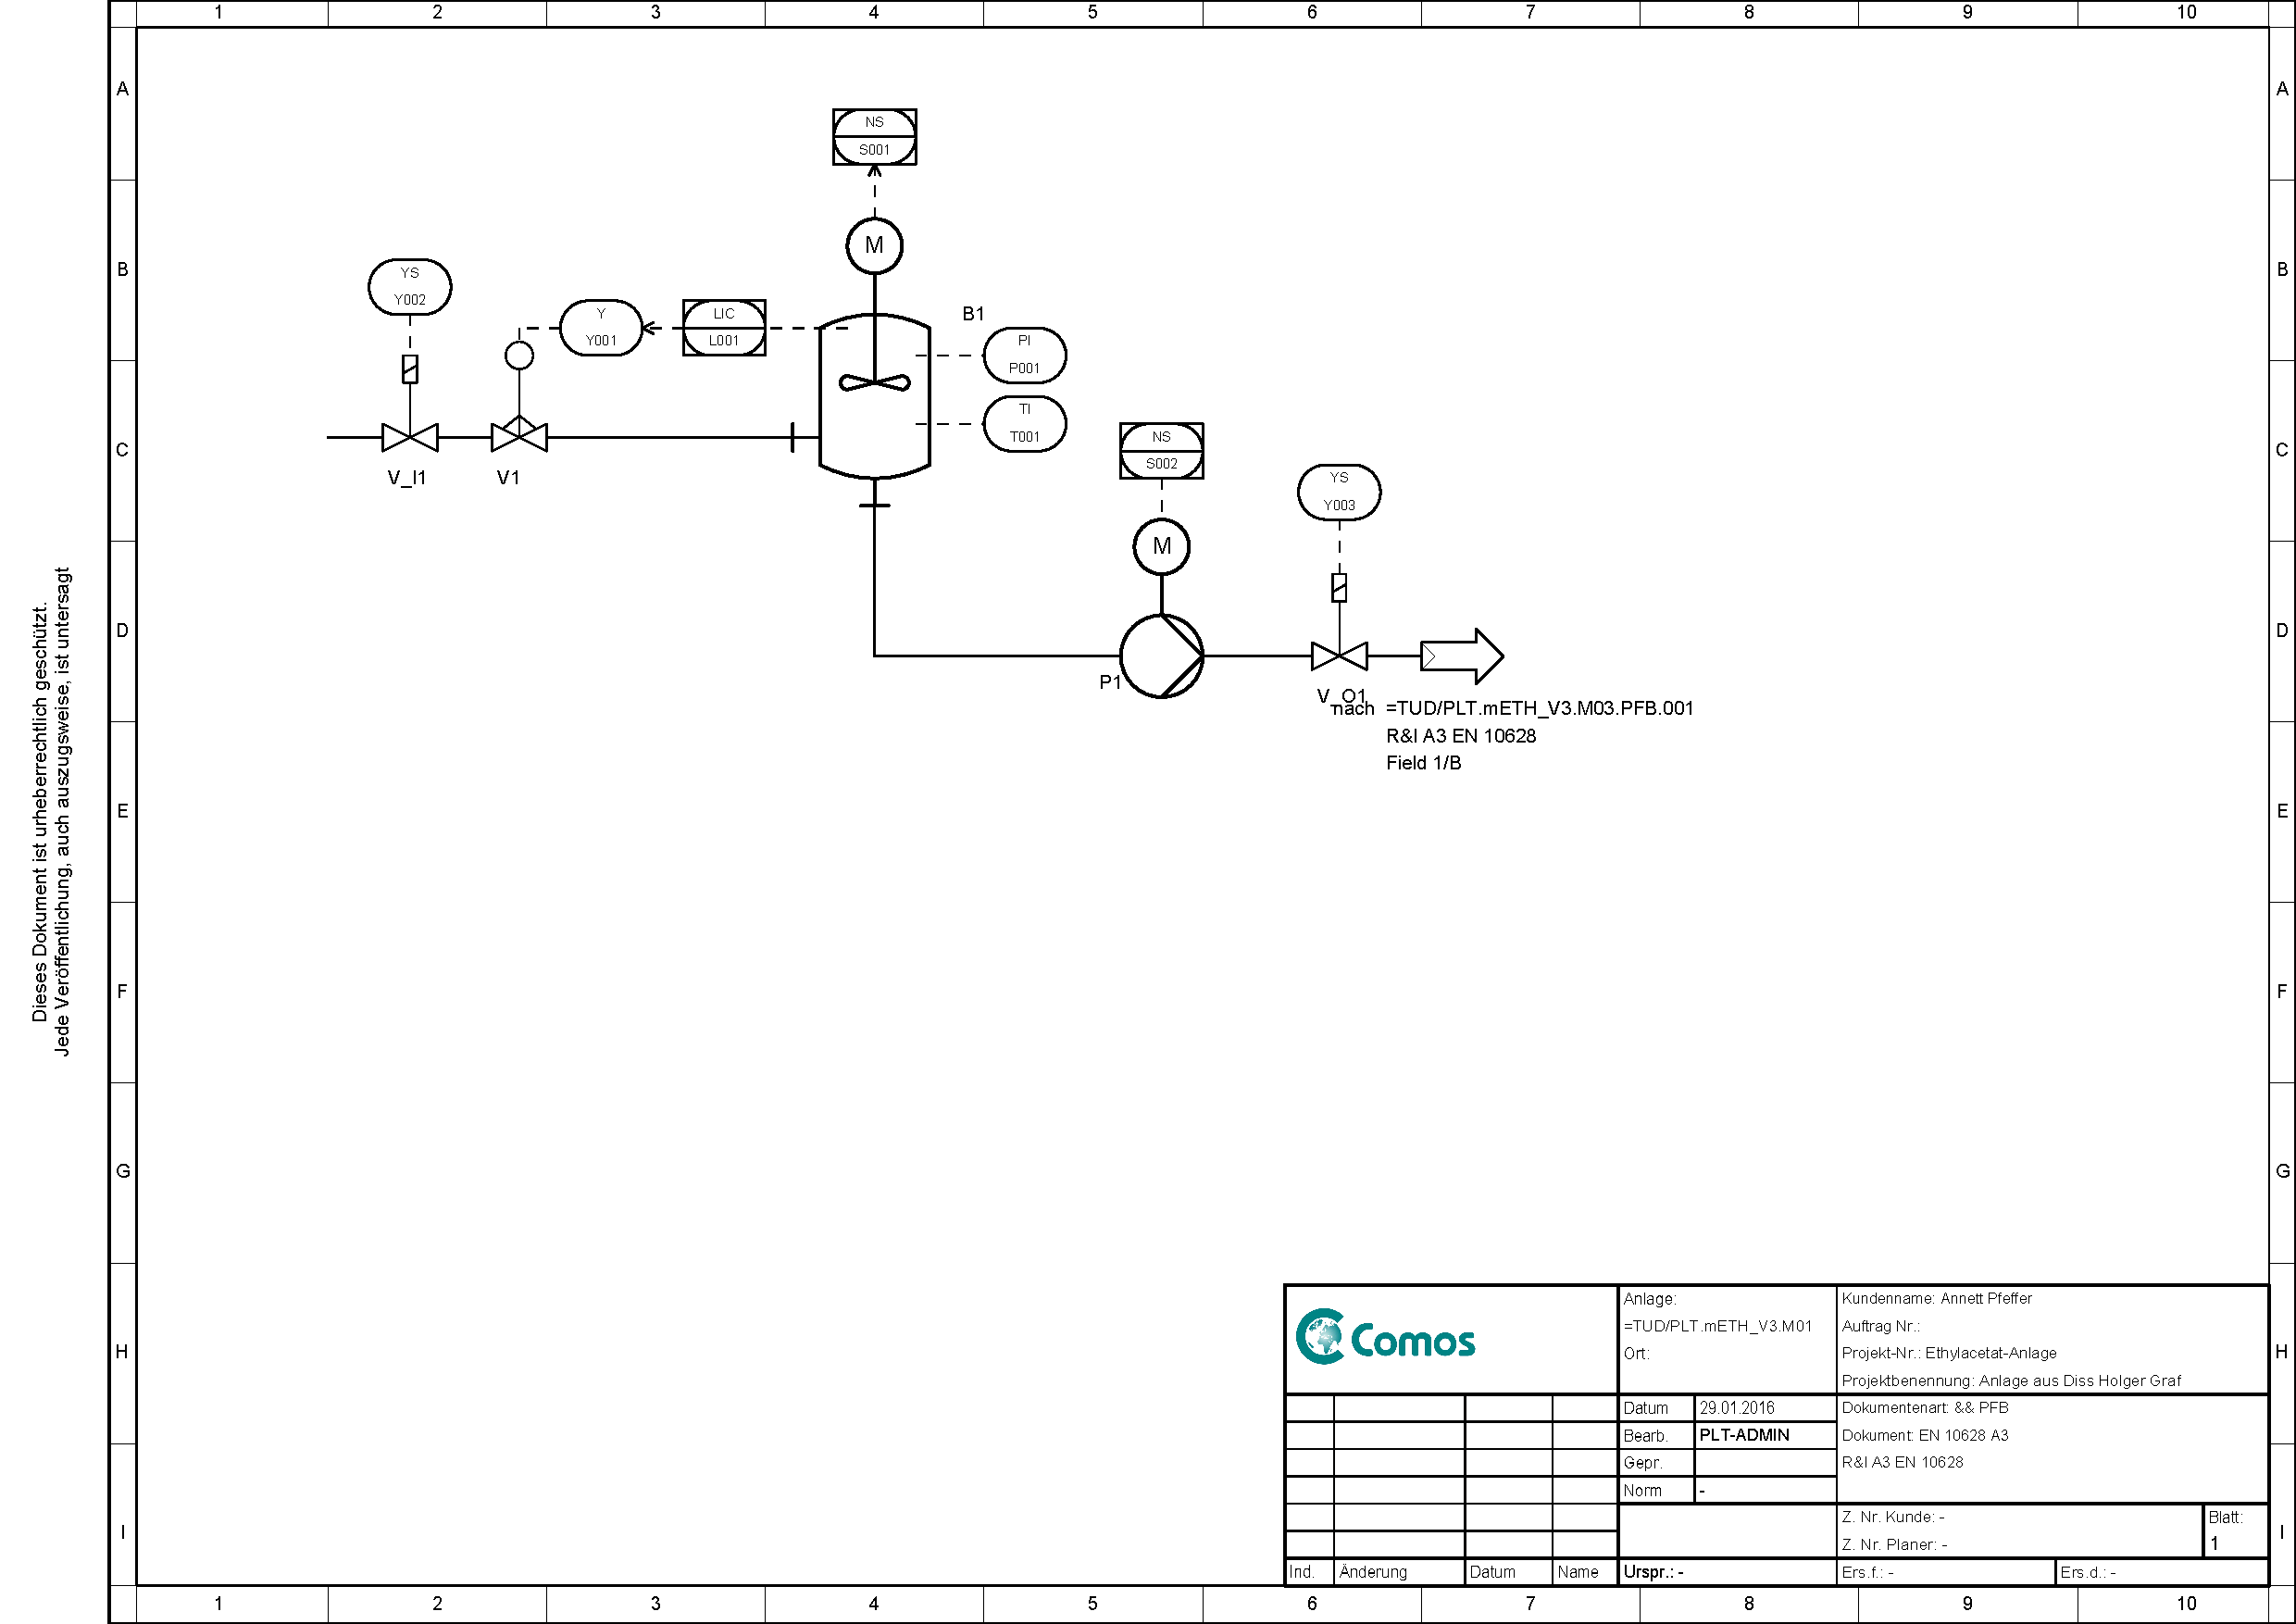
\includegraphics[height=\textwidth,angle=90]{bilder/M01_Vorlage_1_mit_Pumpe.pdf}
\caption[PID Modul 1]{Vorlagemodul 1 nach \cite{Pfeffer_2016}}
\label{fig:PIDMod1}
\end{figure}

\begin{figure}[h!tb]
\centering
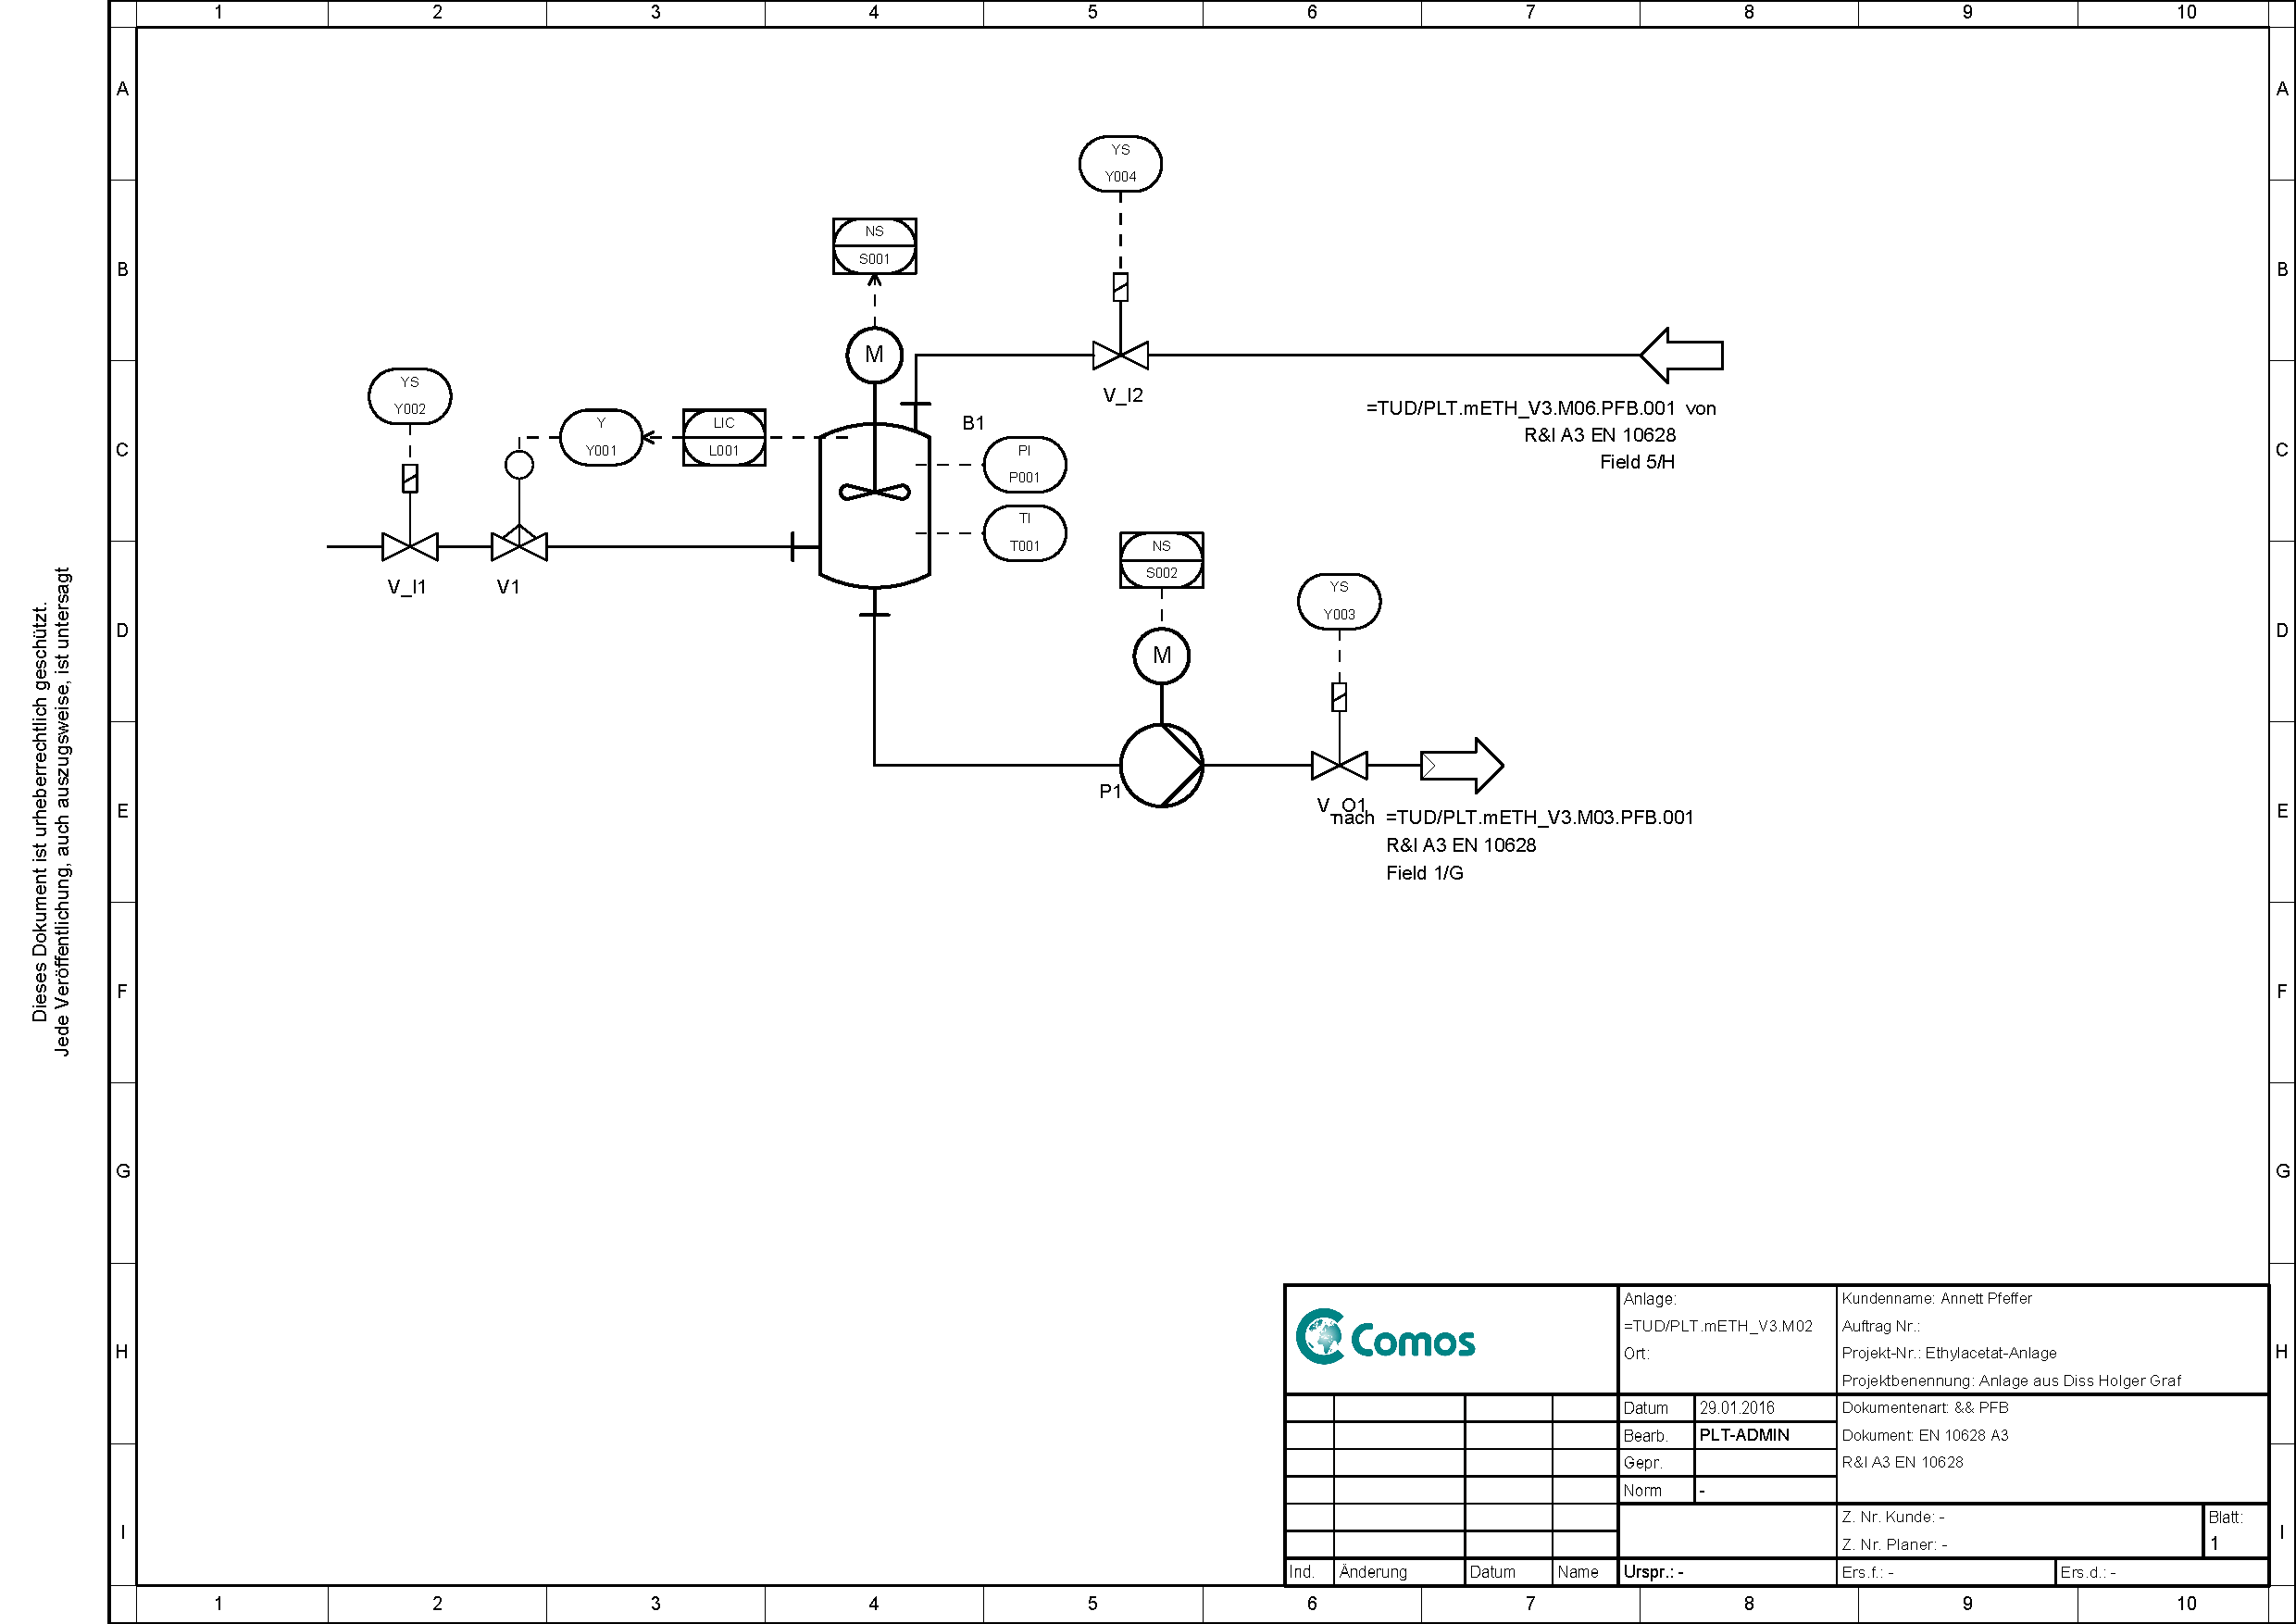
\includegraphics[height=\textwidth,angle=90]{bilder/M02_Vorlage_2_mit_Pumpe.pdf}
\caption[PID Modul 2]{Vorlagemodul 2 nach \cite{Pfeffer_2016}}
\label{fig:PIDMod2}
\end{figure}

\begin{figure}[h!tb]
\centering
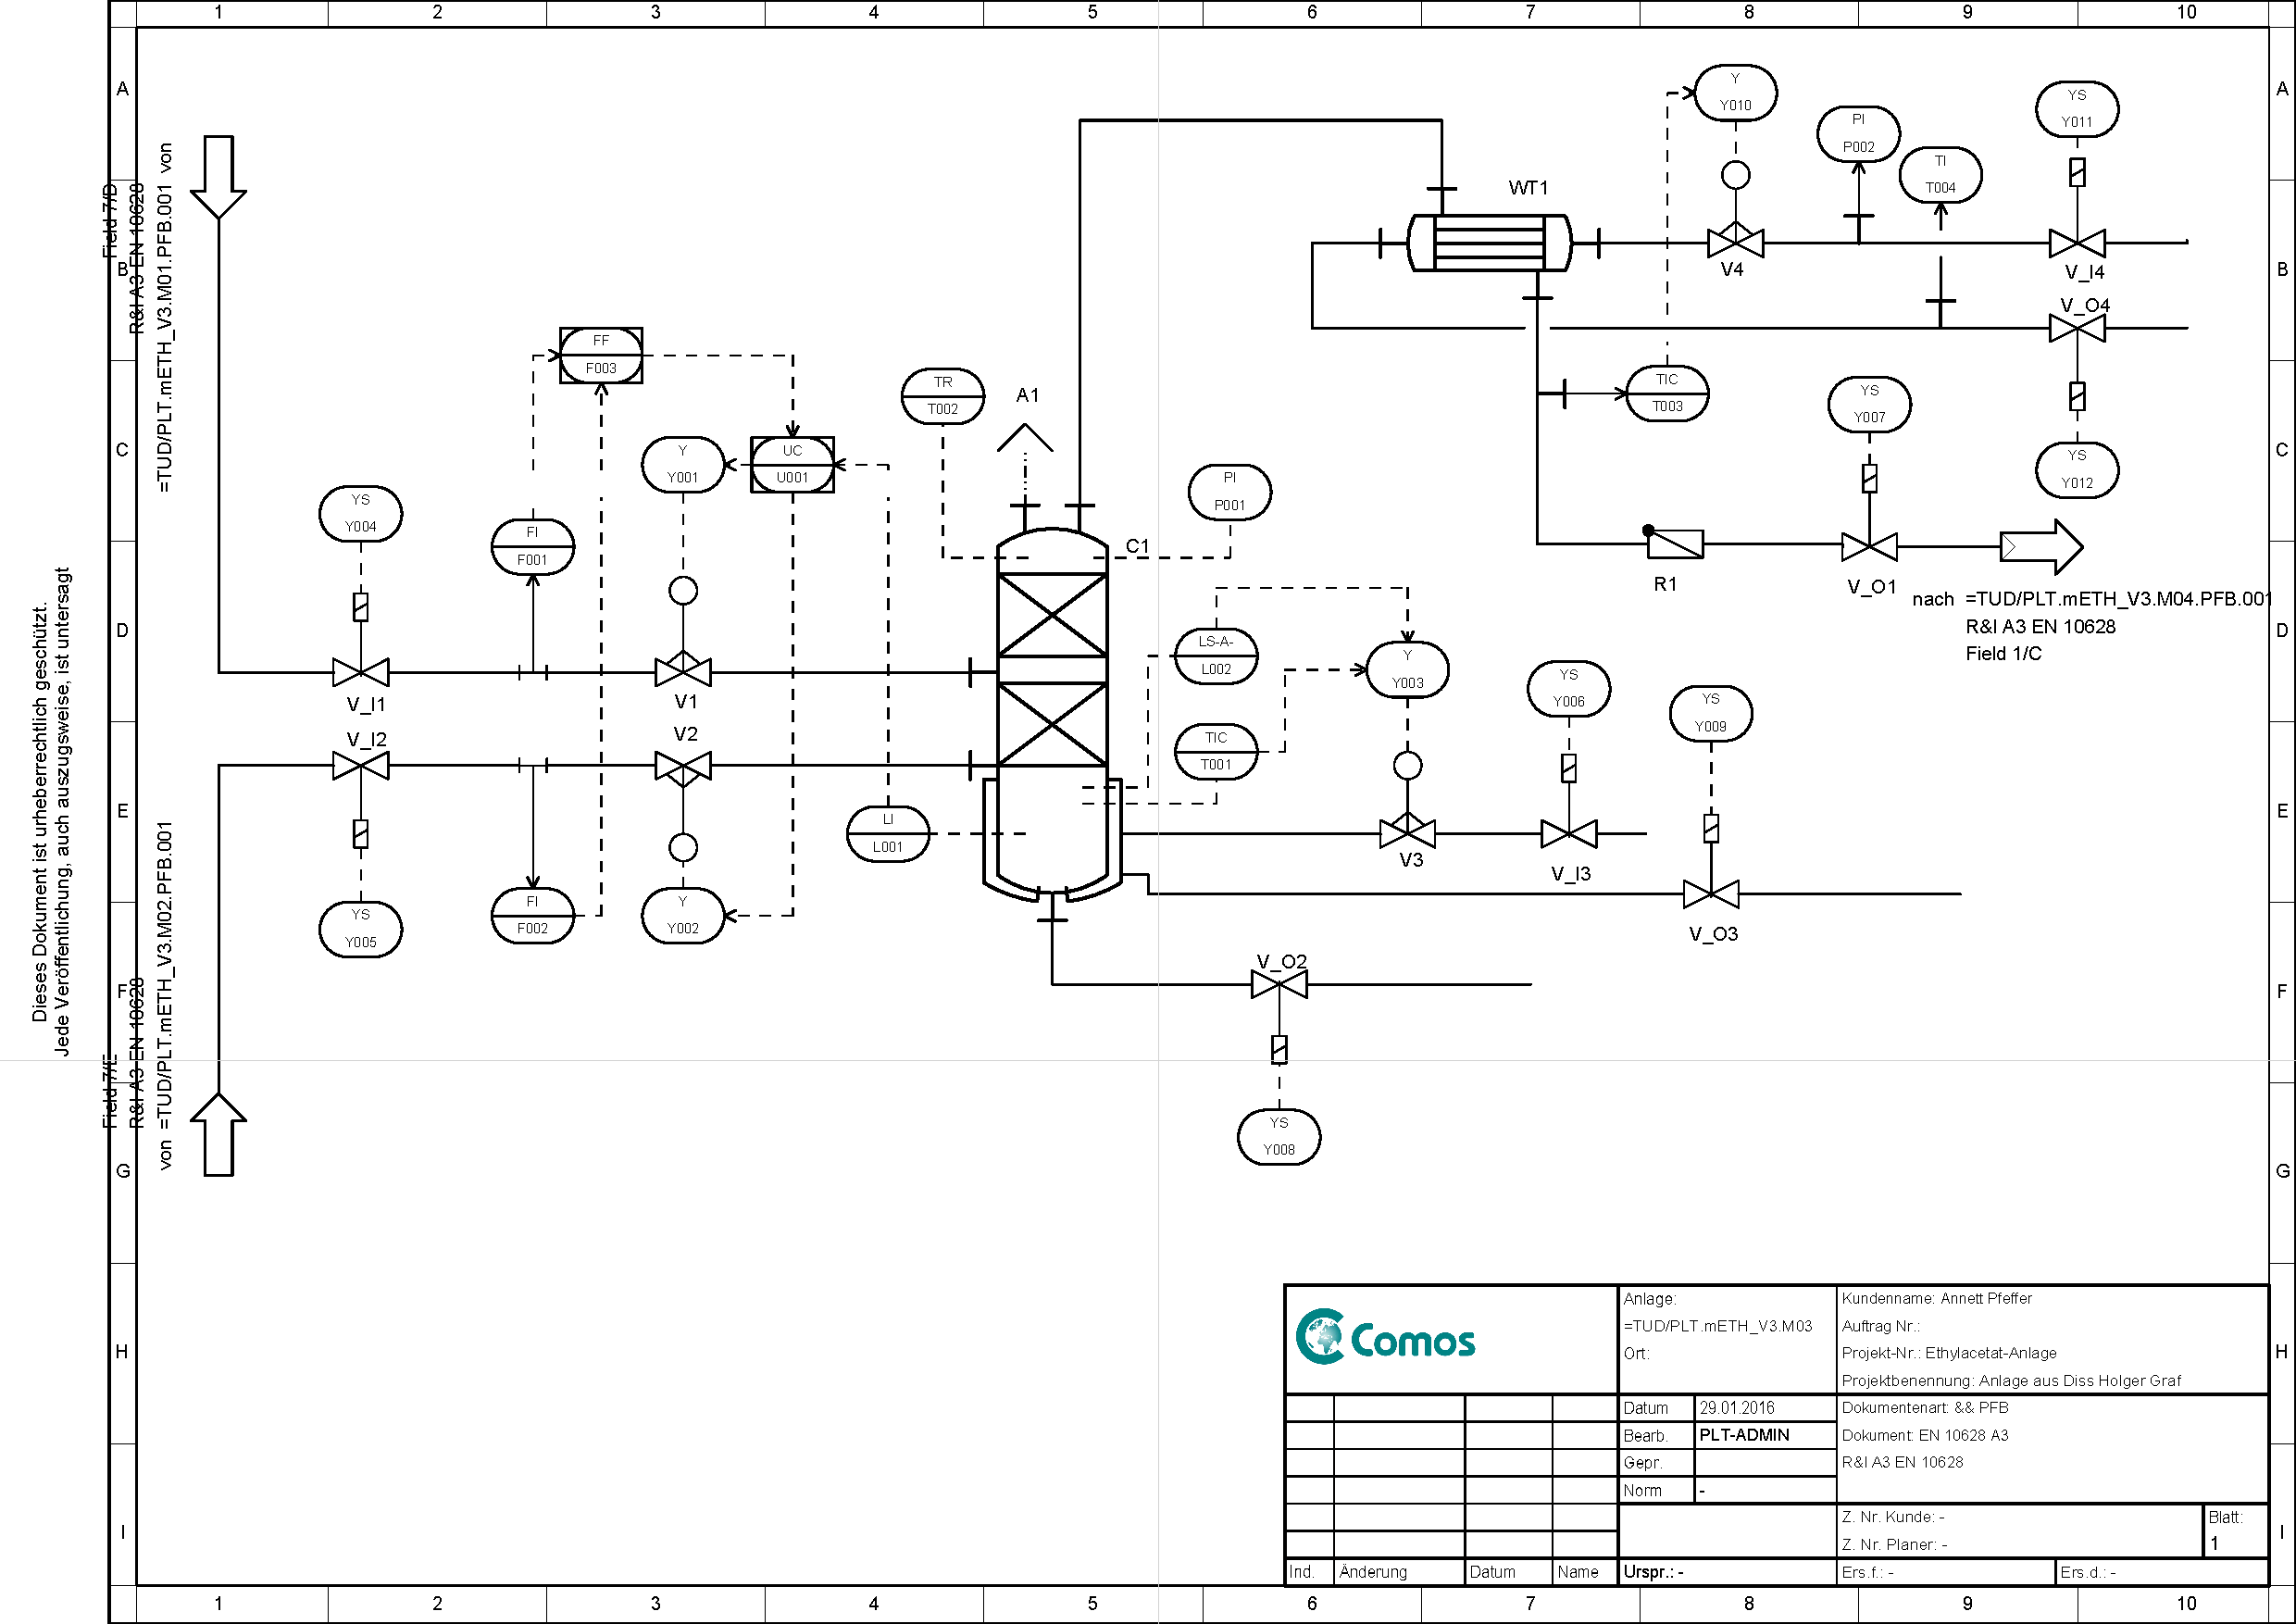
\includegraphics[height=\textwidth,angle=90]{bilder/M03_Kolonne_mit_Waermetauscher.pdf}
\caption[PID Modul 3]{Kolonne mit W\"armetauscher als Modul 3 nach \cite{Pfeffer_2016}}
\label{fig:PIDMod3}
\end{figure}

\begin{figure}[h!tb]
\centering
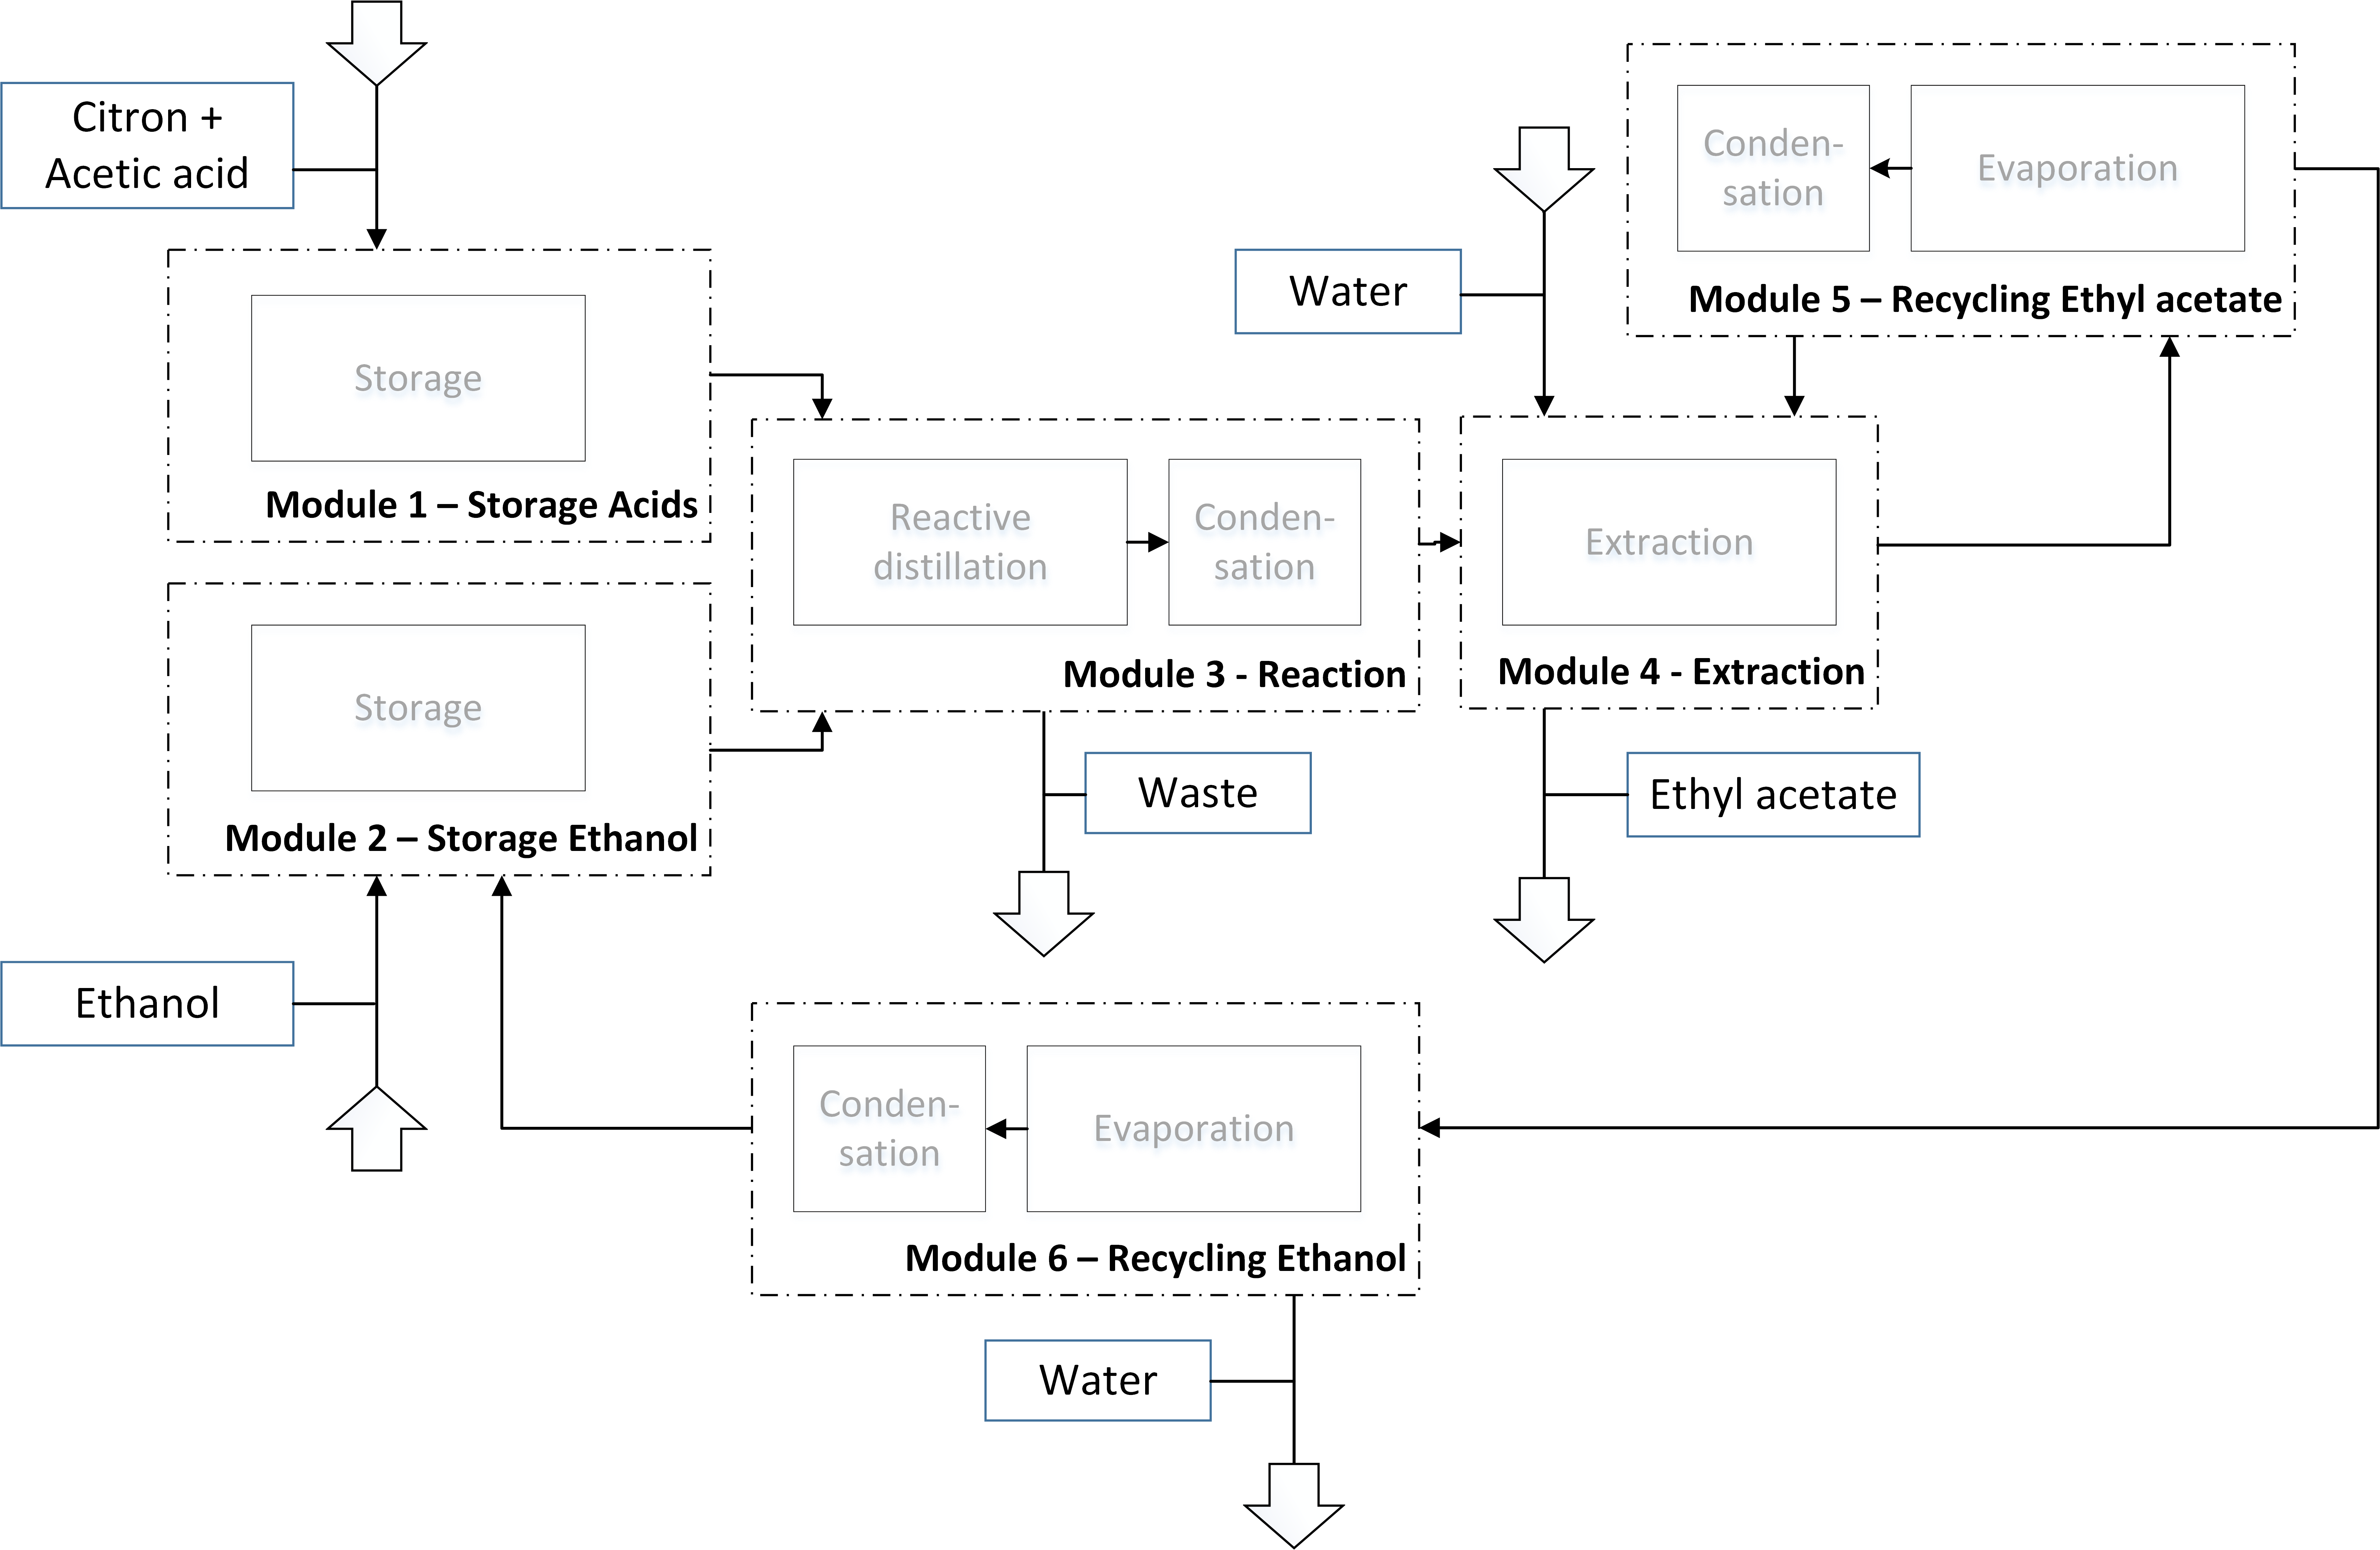
\includegraphics[width=\textheight,angle=90]{bilder/mETH_V3_eng.png}
\caption[Modulare Gesamtanlage]{Darstellung der Ethylacetatanlage als modulare Anlage nach \cite{Pfeffer_2016}}
\label{fig:PIDGes}
\end{figure}

\chapter{Anhang von Tabellen} \label{cha:anhang_tabellen}
\begin{sidewaystable}[htb]
\tablestyle
\caption[HAZOP von Modul 1]{Ergebnisse der \ac{hazop} f\"ur das Tankmodul bezogen auf Durchfluss und F\"ullstand nach \cite{Pfeffer_2017}}
\begin{tabularx}{\textheight}{ccccCCCC}
\tableheadcolor
   {\tablehead ID} &
   {\tablehead unit} &
   {\tablehead Guide word} &
   {\tablehead Physical property} &
   {\tablehead consequences}&
   {\tablehead causes}&
   {\tablehead mechanisms for identification of deviation}&
   {\tablehead recommendation}
   \tabularnewline
%
\tablebody
1	&	in1	&	no	&	flow	&	less tanklevel	&	valve(s) faulty OR control faulty OR externalcauses	&	-	&	-	\\ \hline
2	&	in1	&	more	&	flow	&	more tanklevel	&	valve faulty OR control faulty OR externalcauses	&	-	&	-	\\ \hline
3	&	in1	&	less	&	flow	&	less tanklevel	&	valve(s) faulty OR control faulty OR externalcauses	&	-	&	-	\\ \hline
4	&	tank	&	more	&	level	&	more pressure	&	ID=2 OR level sensor faulty	&	measure level	&	-	\\ \hline
5	&	tank	&	no	&	level	&	no reactant AND damage pump OR less out1flow	&	ID=1 OR ID=3 OR level sensor faulty OR leakage	&	measure level	&	-	\\ \hline
6	&	out1	&	no/less	&	flow	&	damage pump OR external consequences	&	pump faulty OR valve faulty OR ID=5	&	-	&	-	\\ \hline
7	&	out1	&	more	&	flow	&	damage pump OR external consequences	&	pump faulty OR ID=4 OR ID=6	&	-	&	-	\\ \hline
8	&	out1	&	reverse	&	flow	&	pollution of reactant	&	pump faulty OR externalcauses	&	-	&	-
   \tabularnewline
%
\tableend
\end{tabularx}
\label{tab:hazopBsp_M1}
\end{sidewaystable}

\begin{sidewaystable}[htb]
\tablestyle
\caption[HAZOP von Modul 2 Fehlerbehaftet]{Ergebnisse der \ac{hazop} f\"ur das Tankmodul 2 bezogen auf Durchfluss und F\"ullstand mit syntaktischen Abweichungen nach \cite{Pfeffer_2017}}
\begin{tabularx}{\textheight}{ccccCCCC}
\tableheadcolor
   {\tablehead ID} &
   {\tablehead unit} &
   {\tablehead Guide word} &
   {\tablehead Physical property} &
   {\tablehead consequences}&
   {\tablehead causes}&
   {\tablehead mechanisms for identification of deviation}&
   {\tablehead recommendation}
   \tabularnewline
%
\tablebody
1	&	in1	&	no	&	flow	&	less level	&	valve(s) faulty OR control faulty OR externalcauses	&	-	&		\\ \hline
2	&	in1	&	more	&	flow	&	more level	&	valve faulty OR control faulty OR externalcauses	&	-	&		\\ \hline
3	&	in1	&	less	&	flow	&	less level	&	valve(s) faulty OR control faulty OR externalcauses	&	-	&		\\ \hline
4	&	tank	&	more	&	level	&	more pressure (see ID=6)	&	ID=2 OR level sensor faulty	&	measure level	&		\\ \hline
5	&	tank	&	no/less	&	level	&	no reactant $\longrightarrow$ damage pump	&	ID=1 OR ID=3 OR level sensor faulty OR leakage	&	measure level	&		\\ \hline
6	&	out1	&	no/less	&	flow	&	damage pump OR external consequences	&	pump faulty OR valve faulty OR ID=5	&	-	&		\\ \hline
7	&	out1	&	more	&	flow	&	damage pump OR external consequences	&	pump faulty OR ID=4 OR ID=6	&	-	&		\\ \hline
8	&	out1	&	reverse	&	flow	&	pollution of reactant	&	pump faulty OR externalcauses	&	-	&		
   \tabularnewline
%
\tableend
\end{tabularx}
\label{tab:hazopBsp_M2Fehler}
\end{sidewaystable}

\begin{sidewaystable}[htb]
\tablestyle
\caption[HAZOP von Modul 3]{Ergebnisse der \ac{hazop} f\"ur das Modul 3 bestehend aus Kolonne und W\"armetauscher bezogen auf Durchfluss und F\"ullstand nach \cite{Pfeffer_2017}}
\begin{tabularx}{\textheight}{ccccCCCc}
\tableheadcolor
   {\tablehead ID} &
   {\tablehead unit} &
   {\tablehead Guide word} &
   {\tablehead Physical property} &
   {\tablehead consequences}&
   {\tablehead causes}&
   {\tablehead mechanisms for identification of deviation}&
   {\tablehead recommendation}
   \tabularnewline
1	&	in1	&	no	&	flow	&	unknown (no reaction?)	&	valve(s) faulty OR flow/level control faulty OR external causes	&	measure flow	&	-	\\ \hline
2	&	in1	&	more	&	flow	&	changed reaction balance	&	valve(s) faulty OR flow/level control faulty OR external causes	&	measure flow	&	-	\\ \hline
3	&	in1	&	less	&	flow	&	changed reaction balance	&	valve(s) faulty OR flow/level control faulty OR external causes	&	measure flow	&	-	\\ \hline
4	&	in2	&	no	&	flow	&	no reaction	&	valve(s) faulty OR flow/level control faulty OR external causes	&	measure flow	&	-	\\ \hline
5	&	in2	&	more	&	flow	&	changed reaction balance	&	valve(s) faulty OR flow/level control faulty OR external causes	&	measure flow	&	-	\\ \hline
6	&	in2	&	less	&	flow	&	changed reaction balance	&	valve(s) faulty OR flow/level control faulty OR external causes	&	measure flow	&	-	\\ \hline
7	&	coloumn	&	more	&	level	&	changed reaction balance	&	ID=2 OR ID=5	&	measure level	&	-	\\ \hline
8	&	coloumn	&	less	&	level	&	changed reaction balance	&	ID=1 OR ID=3 OR ID=4 OR ID=6 OR leakage 	&	measure level	&	-	
\tablebody
   \tabularnewline
%
\tableend
\end{tabularx}
\label{tab:hazopBsp_M3}
\end{sidewaystable}


%%\begin{table}[h!tb] %if possible put table here else at top or bottom of page
%%\centering %Tabelle wird auf der Seite zentriert
%%%\begin{tabularx}{<width}>{<preambel>}
%%\begin{tabularx}{\linewidth}{@{\extracolsep{\fill}}X|X|X|X|X|X|X@{\extracolsep{\fill}}} %make table as wide as text
%%\toprule %Tabellenanfang
%%% Kopfzeile
%%ID & unit & deviation & causes & consequences & mechanisms for
%%identification of deviation & recommendations \\
%%\midrule %Trennung von Kopf und Inhalt
%%% Inhalt
%%1 & in 1 & less flow & valve(s) faulty (closed, less open, clogged) & less level & - & - \\
%%\bottomrule %Tabellenschluss
%%\end{tabularx}
%%\caption{Ergebnisse einer \ac{hazop} f\"ur einen Tank}
%%\label{tab:hazopBsp} %reference with \prettyref{tab:•}
%%\end{table} 
%\begin{sidewaystable}[htb]
%\tablestyle
%\caption{Ergebnisse einer \ac{hazop} f\"ur einen Tank}
%%\begin{tabularx}{\textwidth}{*{10}{>{\centering\arraybackslash}X}}%
%%\begin{tabularx}{\textheight}{M{0.25cm}M{0.35cm}YM{2.1cm}YM{4.1cm}M{5.1cm}Y}
%\begin{tabularx}{\textheight}{ccccCCCC}
%\tableheadcolor
%%   \multicolumn{1}{c}{\tablehead ID} &
%%   \multicolumn{1}{c}{\tablehead unit} &
%%   \multicolumn{1}{c}{\tablehead Guide word} &
%%   \multicolumn{1}{c}{\tablehead \parbox{2.0cm}{Physical \newline property}} &
%%   \multicolumn{1}{c}{\tablehead consequences}&
%%   \multicolumn{1}{c}{\tablehead \parbox{4.0cm}{causes}}&
%%   \multicolumn{1}{c}{\tablehead \parbox{5cm}{mechanisms for \newline identification of deviation}}&
%%   \multicolumn{1}{c}{\tablehead recommendation}
%%   \tabularnewline
%%    \multirow{2}{*}{\tablehead ID} &
%%    \multirow{2}{*}{\tablehead unit} &
%%    {\tablehead Guide} &
%%    {\tablehead Physical} &
%%    \multirow{2}{*}{\tablehead consequences} &
%%    \multirow{2}{*}{\tablehead causes} &
%%    {\tablehead mechanisms for}&
%%    \multicolumn{1}{c}{\tablehead recommendation} \\
%%
%%    &
%%    &
%%    {\tablehead word}&
%%    {\tablehead property}&
%%    &
%%    &
%%    {\tablehead identification of deviation} &  
%   {\tablehead ID} &
%   {\tablehead unit} &
%   {\tablehead Guide word} &
%   {\tablehead Physical property} &
%   {\tablehead consequences}&
%   {\tablehead causes}&
%   {\tablehead mechanisms for identification of deviation}&
%   {\tablehead recommendation}
%   \tabularnewline
%%
%\tablebody
%  1 & in1 & no & flow & less level & valve(s) faulty OR control faulty OR externalcauses & - & - \\
%  \hline 
%  2 & in1 & more & flow & more level & valve faulty OR control faulty OR externalcauses & - & -  \\ 
%  \hline 
%  3 & in1 & less & flow & less level & valve(s) faulty OR control faulty OR externalcauses & - & - \\ 
%  \hline 
%  4 & tank & more & level & more pressure & ID=2 OR level sensor faulty & measure level & - \\ 
%  \hline 
%  5 & tank & no/less & level & no reactant $\mapsto$ damage pump & ID=1 OR ID=3 OR level sensor faulty OR leakage & measure level & - \\
%  \hline  
%  6 & out1 & no/less & flow & damage pump OR external consequences & pump faulty OR valve faulty OR ID=5 & - & - \\ 
%  \hline 
%  7 & out1 & more & flow & damage pump OR external consequences & pump faulty OR ID=4 OR ID=6 & - & - \\ 
%  \hline 
%  8 & out1 & reverse & flow & pollution of reactant & pump faulty OR external causes & - & - 
%   \tabularnewline
%%
%\tableend
%\end{tabularx}
%\label{tab:hazopBsp}
%\end{sidewaystable}
%
%\IfDefined{printindex}{\printindex}
%\IfDefined{printnomenclature}{\printnomenclature}
%\cleardoublepage
%\leerseite{}
%\cleardoublepage


\end{document}

